\documentclass[10pt]{article}
\usepackage{commands}


\begin{document}
\begin{tcolorbox}
  \begin{center}
  \begin{Large}
    \textbf{PHYS 500 (Quantum Mechanics I) Notes} \\
    \vspace{5pt}
  \end{Large}
  \begin{large}
        Rio Weil \\
\vspace{5pt}
    \emph{This document was typeset on \today}
  \end{large}
  \end{center}
\end{tcolorbox}

\begin{center}
  \textbf{Introduction:}

  This is a set of lecture notes taken from UBC's PHYS 500 (Graduate Quantum Mechanics I) course, taught by Dr.\ Ariel Zhinitsky. The course covers Angular momentum and spin, electromagnetic interactions, Time-independent perturbation theory, the WKB approximation, Time-dependent perturbation theory, the adiabatic approximation, and scattering. If any errors are found in the notes, feel free to email me at \href{mailto:ryoheiweil@phas.ubc.ca}{ryoheiweil@phas.ubc.ca}.

\end{center}
\addtocontents{toc}{\protect\hypertarget{toc}{}}
\tableofcontents

\newpage
\section{Angular Momentum}

\subsection{Units}
We set $\hbar = 1$ for this course (natural units), unless we are doing a numerical estimate of some quantity.

\subsection{Angular Momentum - Definitions}
Angular momentum operators obey the commutation relations:
\begin{equation}
    [L_i, L_j] = i\e_{ijk}L_k.
\end{equation}
Where $\e_{ijk}$ is the Levi-Cicata symbol, defined as:
\begin{equation}
    \e_{ijk} = \begin{cases}
        +1 & ijk \text{ is an even permutation of 123}
        \\ -1 & ijk \text{ is an odd permutation of 123}
        \\ 0 & \text{otherwise}
    \end{cases}
\end{equation}
We also follow the Einstein summation convention, where repeated indices are implicitly summed over. We also define the raising/lowering operators:
\begin{equation}
    L_{\pm} = L_x \pm iL_y
\end{equation}
and the total angular momentum:
\begin{equation}\label{eq-Lsquared}
    \v{L}^2 = L_x^2 + L_y^2 + L_z^2.
\end{equation}
It can be easily verified that:
\begin{equation}
    [\v{L}^2, L_i] = 0
\end{equation}
and that:
\begin{equation}
    [L_z, L_+] = [L_z, L_x + iL_y] = +L_+
\end{equation}
\begin{equation}
    [L_z, L_-] = -L_-
\end{equation}
\begin{equation}
    [\v{L}^2, L_\pm] = 0
\end{equation}
Note that while $L_i$ are Hermitian operators (they are observables), the $L_\pm$ are not (this can be verified by the definition of the Hermitian conjugate). However this does not mean that it is not useful. Now, we ask, what is the physical meaning of:
\begin{equation}
    [\v{L}^2, L_z] = 0
\end{equation}
The answer is that we can know/measure $\v{L}^2$ and $L_z$ simultaneously. Next, what is the meaning of:
\begin{equation}
    [\v{L}^2, L_\pm] = 0
\end{equation}
This means that if we apply $L_{\pm}$ to an eigenstate of $\v{L}^2$, we do not change the eigenstate. Now, what is the physical meaning of:
\begin{equation}
    [L_z, L_+] = L_+?
\end{equation} 
It tells us that $L_+$ is a raising operator for $L_z$; it increments the eigenvalue of $L_z$. 

\subsection{Angular Momentum - Eigenvalues}
Let us now proceed with our construction. Consider the simultaneous eigenbasis of $\v{L}^2$ and $L_z$. Let us call the kets of this eigenbasis as $\ket{l, m}$. We want to solve the eigenvalue problem:
\begin{equation}
    \begin{split}
        \v{L}^2\ket{l, m} &= \lambda\ket{l, m}.
        \\ L_z\ket{l, m} &= m\ket{l, m}
    \end{split}  
\end{equation}
Let us back up for a moment; why can we define a simultaneous eigenbasis? Of course this follows from the fact that $\v{L}^2$ and $L_z$ commute:
\begin{equation}
    [\v{L}^2, L_z] = 0 \implies [\v{L}^2, L_z]\ket{l, m} = 0.
\end{equation}
Let us also check our physical interpretation of $L_+$. We know that $L_+\ket{l, m}$ should give us another eigenstate of $\v{L}^2$ and $L_z$ (which we can call $\ket{x}$), but to this end we calculate:
\begin{equation}
    [\v{L}^2, L_\pm] = 0 \implies [\v{L}^2, L_\pm]\ket{l, m} = 0.
\end{equation}
so we know that:
\begin{equation}
    \v{L}^2\ket{x} - \lambda\ket{x} = 0.
\end{equation}
Now, we know that $[L_z, L_+] = L_+$, so:
\begin{equation}
    [L_z, L_+]\ket{l, m} = L_+\ket{l, m}.
\end{equation}
Expanding the above, we have:
\begin{equation}
    L_z\ket{x} - m\ket{x} = \ket{x}.
\end{equation}
So rearranging we have:
\begin{equation}
    L_z\ket{x} = (m+1)\ket{x}
\end{equation}
And we can find an analogous result for $L_-$. We don't yet know how to normalize these states (we will do so later). But the above result is purely algebraic; no differential equations or spherical harmonics to be found. Let us continue and find the eigenvalues in an algebraic manner. If we recall the definition of $\v{L}^2$ in Eq. \eqref{eq-Lsquared}, we have:
\begin{equation}
    \v{L}^2 = L_z^2 + L_y^2 + L_x^2 = L_z^2 + (L_x + iL_y)(L_x - iL_y) + i(L_xL_y - L_yL_x). 
\end{equation}
Now using what we know of the angular momentum commutation relations and the raising/lowering operators:
\begin{equation}
    \v{L}^2 = L_z^2 + L_+L_- - L_z = L_z^2 + L_-L_+ + L_z
\end{equation}
Now, we consider applying the lowering operator $L_-$ many many times. We then get to a state with the lowest projection $m_{min}$. We then have that:
\begin{equation}
    L_-\ket{l, m_{min}} = 0.
\end{equation}
This arises from the fact that we cannot decrease $m$ further than the total angular momentum value (much in the same way that we cannot go below the ground state of the quantum harmonic oscillator). Analogously, we have:
\begin{equation}
    L_+\ket{l, m_{max}} = 0.
\end{equation}
Now, we apply $\v{L}^2$ to the minimum projection eigenstate. Then using the form of $\v{L}^2$ derived above, we have:
\begin{equation}
    \v{L}^2\ket{l, m_{min}} = (L_z^2 + L_+L_- - L_z)\ket{l, m_{min}}  = (L_z^2 - L_z)\ket{l, m_{min}} = (m^2_{min} - m_{min})\ket{l, m_{min}}
\end{equation}
and analogously:
\begin{equation}
    \v{L}^2\ket{l, m_{max}} = (L_z^2 + L_-L_+ + L_z)\ket{l, m_{max}}  = (L_z^2 + L_z)\ket{l, m_{max}} = (m^2_{max} + m_{max})\ket{l, m_{max}}.
\end{equation}
From this we obtain that:
\begin{equation}
    (m^2_{min} - m_{min}) = (m^2_{max} + m_{max})
\end{equation}
as the magnitude/eigenvalue of $\v{L}^2$ on the min/max projections should be the same. The above equation only has one nontrivial solution:
\begin{equation}
    m_{max} = -m_{min}.
\end{equation}
Now, we observe that we have an integer number of steps (as $L_+/L_-$ raise/lower by integers), so:
\begin{equation}
    m_{max} - m_{min} = N \in \NN
\end{equation}
And therefore:
\begin{equation}
    2m_{max} = N \implies m_{max} = \frac{N}{2}.
\end{equation}
That is to say that the eigenvalues of angular momentum can be integers or half-integers. We can conclude the eigenvalue relations:
\begin{equation}
    \v{L}^2\ket{l, m} = l(l+1)\ket{l, m}
\end{equation}
\begin{equation}
    L_z\ket{l, m} = m\ket{l, m}
\end{equation}
where $l$ or $m$ are either integers or half integers.

Now, we move onto the question of degeneracy. We have a $2l + 1$ degeneracy, where we count:
\begin{equation}
    m = -l, -l + 1, \ldots, 0, \ldots, l - 1, l.
\end{equation}
Now, we suppose we want to compute $\bra{l, m}L_x\ket{l, m}$. It turns out to be zero, but how do we show this? Physically, we can say that $L_x$ is completely uncorrelated with $L_z$ and so we should get zero. Mathematically we can use ladder operators:
\begin{equation}
    \bra{l, m}L_x\ket{l, m} = \bra{l, m}L_+ + L_-\ket{l, m} = \bra{l, m}\left(\ket{l, m+1} + \ket{l, m-1}\right) 0
\end{equation} 
where in the last relation we use that the $\ket{l, m}$ are orthogonal. Now we ask what about $\bra{l, m}L_x^2\ket{l, m}$? It is nonzero. We can calculate this by:
\begin{equation}
    \bra{l, m}L_x^2\ket{l, m} = \bra{l, m}\v{L}^2 - L_z^2 - L_y^2\ket{l, m}
\end{equation}
by symmetry we can conclude that $\bra{l, m}L_x^2\ket{l, m} =\bra{l, m}L_y^2\ket{l, m}$, and so:
\begin{equation}
    \bra{l, m}L_x^2\ket{l, m} = \frac{1}{2}\bra{l, m}(\v{L}^2 - L_z^2)\ket{l, m} = \frac{1}{2}\left[l(l+1) - m^2\right].
\end{equation}
\newpage
\section{Angular Momentum, Continued}
\subsection{Review of Lecture 1}
We start by reviewing the important points of last class. Using the commutation relations for $\v{L}^2, L_z, L_\pm$, we established that $L_\pm$ do not change the eigenvalue of $\v{L}^2$ when acting on an joint eigenstate of $\v{L}^2/L_z$, and we established the equations:
\begin{equation}
    \v{L}^2 = L_z^2 + L_{\pm}L_{\mp} \mp L_z.
\end{equation}
$\v{L}^2$ is the same for the highest and lowest states for $L_z$, and we established that $m_{max} = -m_{min}$. We found that the eigenvalues of $L_z$ jump in integer steps, and can take either integer or half-integer values. The main point is that we derived this purely algebraically (we did not solve Legendre polynomials). Note that 
\begin{equation}
    L_+\ket{l, m_{max}} = L_-\ket{l, m_{min}} = 0
\end{equation}
is equivalent to the boundary conditions when solving this problem in the differential equations approach. We found that:
\begin{equation}
    \bra{l, m}L_{\pm} \ket{l, m} = 0.
\end{equation}
by orthogonality, and using that $L_{x/y} = (L_+ \pm L_-)/2$ that:
\begin{equation}
    \bra{l, m}L_{x/y}\ket{l, m} = \bra{l, m}\frac{L_+ + L_-}{2}\ket{l, m} = 0.
\end{equation}


\subsection{Parity and Pseudovectors}
It is clear that:
\begin{equation}
    \bra{l, m}L_z\ket{l, n} = m.
\end{equation}
We now ask, what is the value of $\bra{l, m}Z\ket{l, m}$ and $\bra{l, m}X\ket{l, m}$? We find that:
\begin{equation}
    \bra{l, m}Z\ket{l, m} = \bra{l, m}X\ket{l, m} = 0
\end{equation}
as when we specify the angular momentum, we know nothing of the position.

How would we do this rigorously? We will come back to this when we do selection rules. For now, let us consider defining the parity operator $P$ that takes a vector $\v{v}$ and maps it to $-\v{v}$. So, each of the position operators get mapped to their negative (i.e. $P^\dagger XP= -X$). Using this in tandem with the fact that $\ket{l, m}$ are eigenvalues of parity (with eigenvalues $(-1)^l$, as we will discuss below), we could conclude that the above expectation values vanish, as:
\begin{equation}
    \bra{l, m} X \ket{l, m} = \bra{l, m}(-1)^l X (-1)^l \ket{l, m} = \bra{l, m}P^\dagger X P\ket{l, m} = \bra{l, m}(-X)\ket{l, m} = -\bra{l, m}X\ket{l, m}
\end{equation}
and comparing the first and last expressions we find that the expectation value is zero. However, we may then ask why does the expectation value of $L_z$ not vanish? This is because angular momentum (like torque and magnetic fields) are not vectors, but rather pseudovectors.

\subsection{Parity Spherical harmonics}
A last note about the eigenkets of angular momentum. In the position basis, we can write them as spherical harmonics:
\begin{equation}
    \ket{l, m} \cong Y_{l}^m(\theta, \phi).
\end{equation}
Consider a unit vector in 3d:
\begin{equation}
    \hat{n} = (n_x, n_y, n_z) = (\sin\theta\cos\phi, \sin\theta\sin\phi, \cos\theta).
\end{equation}
How do the spherical harmonics behave under $Y_l^m(\hat{n}) \to Y_l^m(-\hat{n})$ (in terms of angles, $\theta \to \pi - \theta, \phi \to \phi + \pi$) They transform as:
\begin{equation}
    Y_l^m(-\hat{n}) = (-1)^lY_{l}^m(\hat{n}).
\end{equation}
Let us look at a couple examples. $Y_0^0 \sim \frac{1}{\sqrt{4\pi}}$ so is unchanged under the flip of the vector. $Y_1^0 \sim \cos\theta$ so this maps to $\cos(-\theta) \to -\cos\theta$ under a flip of the vector. $Y_1^1 \sim \sin\theta e^{i\phi}$, so the $\sin\theta$ stays the same under interchange but $e^{i\phi}$ flips sign so it maps to $-Y_1^1$. 

Note this discussion is really trying to motivate the use of symmetry to skip doing computations; we don't have to compute integrals if we know the symmetry of the system.

Another example (returning to the above discussion of expectation values of position). Hopefully by now we would be convinced that:
\begin{equation}
    \bra{l, m}\v{R}\ket{l, m}  = 0.
\end{equation}
by the above arguments showing that $\ket{l, m}$ are eigenvalues of parity with eigenvalue $(-1)^l$. Now what about $\bra{l+1, m}\v{R}\ket{l, m}$? In this case it is \emph{nonzero} as the negative signs cancel when we consider the parity properties.

\subsection{Eigenvalues of Ladder Operators}
We know that the ladder operators follow the relation:
\begin{equation}
    L_+\ket{l, m} = c_+\ket{l, m+1}
\end{equation}
but we have yet to calculate $c_+$. Let us do this now. We consider acting $L_-$ on the dual of $\ket{l, m}$:
\begin{equation}
    \bra{l, m}L_- = c_+^*\bra{l, m+1}
\end{equation}
So therefore:
\begin{equation}
    \bra{l, m}L_-L_+\ket{l, m} = \abs{c_+}^2\braket{l, m+1}{l, m+1}
\end{equation}
so:
\begin{equation}
    \abs{c_+}^2\bra{l, m}\v{L}^2 - L_z^2 - L_z\ket{l, m} = l(l+1) - m^2 - m
\end{equation}
so we conclude:
\begin{equation}
    c_+ = \sqrt{l(l+1) - m(m+1)}
\end{equation}
and an analogous computation can be done to find $c_-$.

\subsection{Spin 1/2}
Because of the degeneracy of angular momentum ($2l+1$) derived via the Schrodinger equation, people expected to always see an odd number of lines when doing energy line experiments. But this turned out not to be true in experimental results; we require a new approach to the theory, developed by Pauli. We now thus explore spin 1/2 systems. For such systems, we have $s = 1/2$, where the spin operators follow the commutation relations:
\begin{equation}
    [S_i, S_j] = i\e_{ijk}S_k.
\end{equation}
Since there are $(2s+1)$ states, we have only two spin eigenstates:
\begin{equation}
    \ket{s = \frac{1}{2}, s_z = +\frac{1}{2}}, \ket{s = \frac{1}{2}, s_z = -\frac{1}{2}}
\end{equation}
Which obey:
\begin{equation}
    S_+\ket{s = \frac{1}{2}, s_z = +\frac{1}{2}} = 0,  S_-\ket{s = \frac{1}{2}, s_z = -\frac{1}{2}} = 0
\end{equation}
Given this, a natural notation for these states is:
\begin{equation}
    \ket{\uparrow} \coloneqq \ket{s = \frac{1}{2}, s_z = +\frac{1}{2}}, \ket{\downarrow} \coloneqq \ket{s = \frac{1}{2}, s_z = -\frac{1}{2}}
\end{equation}
So the above relations become (e.g.) $S_+\ket{\uparrow} = 0$. The total spin operator is given by:
\begin{equation}
    \v{S} \cong \frac{1}{2}\gv{\sigma}
\end{equation}
where $\gv{\sigma} = (\sigma_x, \sigma_y, \sigma_z)^T$, with the Pauli matrices given by:
\begin{equation}
    \sigma_x = \paulix, \sigma_y = \pauliy, \sigma_z = \pauliz.
\end{equation}
Note that there is no reference to coordinates whatsoever here; everything is purely algebraic. Now, what is the value of $\v{S}^2\ket{\uparrow}$? From the theory of angular momentum, we know that:
\begin{equation}
    \v{S}^2\ket{\uparrow} = s(s+1)\ket{\uparrow} = \frac{3}{4}\ket{\uparrow}.
\end{equation}
But let us derive this result using the matrix form of $\v{S}^2$. We can explicitly calculate to find that:
\begin{equation}
    \sigma_i^2 = \imatrix
\end{equation}
for each of the pauli matrices, so:
\begin{equation}
    \v{S}^2 \cong \frac{1}{4}(\sigma_x^2 + \sigma_y^2 + \sigma_z^2) = \frac{3}{4}\imatrix.
\end{equation}
So with the choice of representation that $\ket{\uparrow} \cong \m{1 \\ 0}$ and $\ket{\downarrow} \cong \m{0\\ 1}$, we find:
\begin{equation}
    \v{S}^2\ket{\uparrow} = \frac{3}{4}\ket{\uparrow},
\end{equation}
along with:
\begin{equation}
    S_z\ket{\uparrow} = \ket{\uparrow}.
\end{equation}
by looking at these matrix expressions. From now on, we will focus on spin-1/2 (though we will explore spin-1 in the homework). We will discuss the most general spin 1/2 state. It is given by:
\begin{equation}
    \ket{\chi} = c_+\ket{\uparrow} + c_-\ket{\downarrow}.
\end{equation}
In the spinor representation, it is given by:
\begin{equation}
    \chi = \m{c_+ \\ c_-}.
\end{equation}
How many real parameters are needed to specify the quantum state? Naively, we would say 4 (2 complex numbers). But it turns out to be only two. One parameter is reduced by the normalization condition:
\begin{equation}
    \abs{c_+}^2 + \abs{c_-}^2 = 1.
\end{equation}
We also have a reduction of one from the fact that the state is physically unchanged when multiplied by a global phase $\ket{\chi} \sim e^{i\phi}\ket{\chi}$; this comes from the fact that we can only measure probabilities in QM, and when we calculate these (using the Born rule, $p(i) = \bra{\psi}\Pi_i\ket{\psi}$ the global phase cancells out). An important distinction: \emph{relative} phases are observable (e.g. in neutron inferometry experiments), while global ones are not. So in the case of a single spin-1/2 particle, we can neglect the phase, but when we have multiple particles we cannot neglect relative phases.

\subsection{Magnetic Hamiltonians}
Consider the Hamiltonian:
\begin{equation}
    \H = -\gv{\mu} \cdot \v{B}.
\end{equation}
Where $\gv{\mu} = \gamma \gv{s}$. This $\gamma$ coefficient cannot be estimated by classical physics; a full calculation requires considering the Dirac field in QFT. But we can also evaluate it via experiment.

Next day, we will continue our discussion of this Hamiltonian and the evolution of spin states under it. We will also discuss Gauge invariance in the context of quantum mechanics.


\newpage
\section{Electron in EM field}
\subsection{Review of Spin}
We have the spin commutation algebra (identical to the angular momentum commutation algebra):
\begin{equation}
    [S_i, S_j] = i\e_{ijk}S_k.
\end{equation}
However, there is no way to represent the spin operators in spatial coordinate; we instead use matrices. Consider $s = 1/2$. Then we have $\v{S} = \frac{1}{2}\gv{\sigma}$, where $S_z$ has eigenstates $\ket{\uparrow} \cong \binom{1}{0}$ and $\ket{\downarrow} \cong \binom{0}{1}$. Any state can be expressed as a linear combination of these two:
\begin{equation}
    \chi = \frac{c_+}{\sqrt{\abs{c_+}^2 + \abs{c_-}^2}}\m{1\\0} + \frac{c_-}{\sqrt{\abs{c_+}^2 + \abs{c_-}^2}}\m{0\\1}.
\end{equation}

\subsection{Inner and Outer Products, Completeness}
We also have the inner product that gives us numbers:
\begin{equation}
    \braket{\uparrow}{\uparrow} = \m{1 & 0}\m{1\\0} = 1.
\end{equation}
Also note that outer products give us matrices:
\begin{equation}
    P_+ = \dyad{\uparrow}{\uparrow} \cong \m{1\\0}\m{1&0} = \m{1&0\\0&0}
\end{equation}
The above $P_\uparrow$ is a projector (that projects onto the spin-up subspace); as we have:
\begin{equation}
    P_\uparrow\ket{\uparrow} = \uparrow, P_+\ket{\downarrow} = 0.
\end{equation}
Note also the completeness relation:
\begin{equation}
    \dyad{\uparrow}{\uparrow} + \dyad{\downarrow}{\downarrow} = \II.
\end{equation}
As $\set{\ket{\uparrow}, \ket{\downarrow}}$ is an ONB for the spin-1/2 Hilbert space. When we have infinitely many states in an ONB, we have:
\begin{equation}
    \sum_{n=0}^\infty \dyad{n}{n} = \mathbb{I}, \quad \int \dyad{x}{x}dx = \mathbb{I}
\end{equation}
where the former is for a discrete ONB, the latter is for a continuous one (of course there are the caveats that $\ket{x}$ aren't really square-integrable states, but let us not worry about this). Now, a question: what is the $\dyad{\uparrow}{\downarrow}$? It is an operator that flips a down-spin to an up-spin:
\begin{equation}
    \dyad{\uparrow}{\downarrow} \cong \m{0&1\\0&0}
\end{equation}
Of course this is just the $S_+$ operator (it is not Hermitian, while $P_\uparrow$ is).

\subsection{Electron in Magnetic Field}
Consider the Hamiltonian:
\begin{equation}
    H = -\gv{\mu}\cdot \v{B}
\end{equation}
where $\gv{\mu} = \gamma\v{S}$ with $\gamma$ is a scalar known as the gyromagnetic ratio. It is equal to:
\begin{equation}
    \gamma = \frac{e\hbar}{2mc}2
\end{equation}
Note we've written $\gamma$ to include the $\hbar$ factor; usually $\hbar$ goes with $\v{S}$, but with our units convention, we prefer to write it this way. Note that if we calculate the gyromagnetic moment just by classical methods, we would just get $\frac{e}{2mc}$. The coefficient $2$ is the $g$-factor, which can be obtained by taking the nonrelativistic limit of the Dirac equation (we won't try to do this here); there is some hidden deep physics here we will leave for a different course.

Note that we have assumed that there is no orbital angular momentum for the electron (we only consider the intrinsic spin); a full treatment would take:
\begin{equation}
    \gv{\mu} = \frac{e\hbar}{2mc}\left(2\v{S} + \v{L}\right).
\end{equation}

\subsection{Electron in Magnetic Field in a single direction}
Now, we suppose a more specific scenario, where $\v{B}$ is aligned along the $z$-axis. We then have:
\begin{equation}
    H = -\gamma B_z\frac{1}{2}\pauliz.
\end{equation}
We have two easily solved eigenvalue equations:
\begin{equation}
    H\chi_+ = E_+\chi_+, H\chi_- = E_-\chi_-.
\end{equation}
Where $E_+ = -\frac{1}{2}\gamma B_z$ and $E_- = \frac{1}{2}\gamma B_z$. Now, a question; why is there a minus sign in $H$? The convention is such that the dipole moment wants to align with the magnetic field. 

Note that in our problem here, the $+$ denotes that we have a upwards projection (and a negative energy, as it is pointed along the field). Conversely, $-$ denotes that we have a downwards projection (and a positive energy). Of course, we know that:
\begin{equation}
    \chi_+ = \m{1\\0}, \chi_- = \m{0\\1}.
\end{equation}
and now everything is solved! We know the eigenvalues and eigenstates, so we have everything we need to determine the Schrodinger time evolution of the quantum state. We can say that:
\begin{equation}
    \chi(t) = \frac{c_+e^{-i\frac{E_+t}{\hbar}}}{\sqrt{\abs{c_+}^2 + \abs{c_-}^2}}\m{1\\0} + \frac{c_-e^{-i\frac{E_-t}{\hbar}}}{\sqrt{\abs{c_+}^2 + \abs{c_-}^2}}\m{0\\1}
\end{equation}

\subsection{Time-dependence of Observables}
For a most general spin-1/2 state, if we enforce the normalization condition of $\abs{c_+}^2 + \abs{c_-}^2 = 1$, then we can parameterize with just three parameters:
\begin{equation}\label{eq-chigeneral}
    \chi = e^{i\alpha}\m{\cos\frac{\theta}{2} \\ \sin\frac{\theta}{2}e^{-i\phi}}
\end{equation}
For now, let us discard the phases ($\alpha = \phi = 0$) and suppose that at $t = 0$ we have:
\begin{equation}\label{eq-chithetat0}
    \chi(t = 0) = \m{\cos\frac{\theta}{2} \\ \sin\frac{\theta}{2}}.
\end{equation}

Question: Let us compute:
\begin{equation}
    \avg{S_z}(t) = \bra{\chi(t)}S_z\ket{\chi(t)}.
\end{equation}
This turns out to be independent of time; let us see this in two ways. First, we can do the explicit calculation. $\chi(t)$ is given by:
\begin{equation}
    \chi(t) = \m{\cos\frac{\theta}{2} e^{i\omega t/2} \\ \sin\frac{\theta}{2} e^{-i\omega t/2}}
\end{equation}
Where $\omega$ is defined as the difference between the two frequencies. When we do the explicit computation, we find:
\begin{equation}
    \bra{\chi(t)}S_z\ket{\chi(t)} = \m{\cos\frac{\theta}{2} e^{-i\omega t/2}& \sin\frac{\theta}{2} e^{i\omega t/2}}\pauliz \m{\cos\frac{\theta}{2} e^{i\omega t/2} \\ \sin\frac{\theta}{2} e^{-i\omega t/2}} =  \frac{1}{2}\left(\cos^2\frac{\theta}{2} - \sin^2\frac{\theta}{2}\right) = \frac{1}{2}\cos\theta.
\end{equation}
If we do the same comnputation for $\avg{S_x}(t)$, we find that the time-dependence does not cancel out:
\begin{equation}
    \bra{\chi(t)}S_x\ket{\chi(t)} = \m{\cos\frac{\theta}{2} e^{-i\omega t/2}& \sin\frac{\theta}{2} e^{i\omega t/2}}\paulix \m{\cos\frac{\theta}{2} e^{i\omega t/2} \\ \sin\frac{\theta}{2} e^{-i\omega t/2}} =  \frac{1}{2}\sin\frac{\theta}{2}\cos\frac{\theta}{2}\left(e^{i\omega t} + e^{-i\omega t}\right) = \frac{1}{2}\sin\theta\cos(\omega t).
\end{equation}
We can picture this as the spin precessing at a fixed angle $\theta$ (fixed $z$-position).

\begin{figure}[htbp]
    \centering
    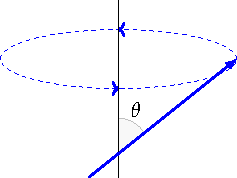
\includegraphics[]{Images/fig-spinprecess.pdf}

    \caption{When the initial spinor state $\chi(t = 0)$ is given by Eq. \eqref{eq-chithetat0} and evolves under a $z$-oriented magnetic field, the spin state can be visualized as precessing at fixed $\theta$ (the same $\theta$ as in the initial state). More technically, we could say that the spin state precesses at a fixed polar angle on the Bloch sphere; Note that the general spin state given in Eq. \eqref{eq-chigeneral} invites the visualization of a single spin-1/2 particle as a point on the unit sphere with polar coordinates $(\theta, \phi)$ (of course the global phase $\alpha$ is physically irrelevant).}
    \label{fig-spinprecess}
\end{figure}

However, there is a \emph{much} easier way to see why there is no time-dependence in the $S_z$ case, while there is a time-dependence in the $S_x$ case. The way to see this is that $[S_z, H] = 0$ ($S_z$ commutes with the Hamiltonian) so there is no time-dependence. Conversely, $S_x$ does not commute with the Hamiltonian, so we know that there is time dependence.

Let us discuss the simple case where:
\begin{equation}
    \chi(t = 0) = \frac{1}{\sqrt{2}}
    \m{1\\1}.
\end{equation}

Now, we want the probability of finding the spin to be in spin-up $P_\uparrow$ as a function of time. In this case, this will again be independent of time; a physical picture is that the spin precesses at a fixed angle, so the projection onto the $s_z$ axis does not change with time. A more concrete argument is that if we measure the probability of getting some outcome of an $S_z$ measurement, since $S_z$ commutes with $H$ then this probability should be independent of time. Let's see how this works out explicitly:
\begin{equation}
    \chi(t) = \frac{1}{\sqrt{2}}\m{1\\0}e^{i\omega t/2} + \frac{1}{\sqrt{2}}\m{0\\1}e^{-i\omega t/2}.
\end{equation}
By the Born rule we have::
\begin{equation}
    P_\uparrow = \abs{\braket{\uparrow}{\chi}}^2 = \frac{1}{2}
\end{equation}
which is time-independent. Let us now ask the probability of measuring $P_{+\xhat}$; how do we proceed? We start by finding the eigenstates of $S_x$:
\begin{equation}
    S_x \ket{\chi_{+\xhat}} = \lambda \ket{\chi_{+\xhat}} \cong \frac{1}{2}\sigma_x\chi_{+\xhat} = \lambda \chi_{+\xhat} \implies \chi_{+\xhat} = \frac{1}{\sqrt{2}}\m{1\\1}.
\end{equation}
We therefore can calculate:
\begin{equation}
    P_{+\xhat} = \abs{\frac{1}{\sqrt{2}}\m{1 & 1}\chi(t)}^2 = \abs{\frac{1}{\sqrt{2}}\m{1 & 1}\frac{1}{\sqrt{2}}\m{e^{i\omega t/2} \\ e^{-i\omega t/2}}}^2 = \abs{\frac{1}{2}\left(e^{i\omega t/2} + e^{-i\omega t/2}\right)}^2 = \frac{1}{2}\left(1 + \cos\omega t\right)
\end{equation}
Because the measurement is dichotomic, we can use completeness to find $P_{-\xhat}$:
\begin{equation}
    P_{-\xhat} = 1 - P_{+\xhat} = \frac{1}{2}\left(1 - \cos\omega t\right).
\end{equation}
\newpage
\section{Electromagnetic Fields}
\subsection{The Hamiltonian and Gaussian units}
We consider the Hamiltonian:
\begin{equation}\label{eq-Hem}
    H = \frac{1}{2m}\left(\v{p} - \frac{q}{c}\v{A}\right)^2 + qV
\end{equation}
We use Gaussian units, where $\frac{e^2}{4\pi \e_0} \to e^2$. The potential will (for the Coulomb interaction) will later be $qV = -\frac{Ze^2}{r}$ (the sign will be relevant later, to distinguish attractive (negative sign) and repulsive). For now take $q = -e$. Note for the magnetic moment we take:
\begin{equation}
    \mu = \frac{\abs{e}\hbar}{2mc}
\end{equation}
why Gaussian units? Because in SI units, the electric and magnetic fields have different units, but in Gaussian, they have the same units. Things will become unbelievably tedious to keep track of if we keep the $4\pi\e_0$s in. The Hydrogen atom Hamiltonian takes the form:
\begin{equation}
    H = \frac{1}{2m}\v{p}^2 - \frac{Ze^2}{r}.
\end{equation}
And to solve this problem, we take $\v{p} \to -i\hbar \nabla$ and use the standard techniques (covered in undergrad QM).

\subsection{Potentials and Gauge Invariance}
Let us make some comments about the Hamilonian in Eq. \eqref{eq-Hem}. We may be familiar with the Lorentz force law in classical E\&M:
\begin{equation}
    m\ddot{\v{r}} = \v{F} = q(\v{E} + \v{v} \times \v{B})
\end{equation}
where the dynamics are completely governed by the fields $\v{E}, \v{B}$. We can specify the fields by the scalar/vector potentials $V/\v{A}$:
\begin{equation}
    \v{B} = \nabla \times \v{A}, \quad \v{E} = -\nabla V - \frac{1}{c}\dpd{\v{A}}{t}.
\end{equation}
$V, \v{A}$ have features known as \emph{Gauge invariance}; a fundamental principle of nature. Consider the gauge transformation:
\begin{equation}
    V' = V - \frac{1}{c}\dpd{f(\v{r}, t)}{t}, \quad \v{A}' = \v{A} + \nabla f(\v{r}, t).
\end{equation}
When we do computations for electric and magnetic fields, we find that $V'/\v{A}'$ specify the same physical fields:
\begin{equation}
    \v{E}' = -\nabla V' - \frac{1}{c}\dpd{\v{A}'}{t} = \v{E} + \left(\dpd{}{t}\nabla  - \nabla \dpd{}{t}\right)f(\v{r}, t) = \v{E}
\end{equation}
and analogously:
\begin{equation}
    \v{B}' = \v{B}.
\end{equation}
In classical physics, this is a triviality; a gauge transformation does nothing to the physics. What about quantum mechanics? In quantum mechanics we solve the SE:
\begin{equation}
    H\psi = E\psi
\end{equation} 
with the Hamiltonian Eq. \eqref{eq-Hem}. Now it begins to seem like we have a different equation; is this indeed the case? 

In classical physics, we tend to fix gauges based on convenience. When we study electrostatics, we choose the Coloumb gauge:
\begin{equation}
    \nabla \cdot \v{A} = 0
\end{equation}
When we study radiation, we choose the Lorentz gauge (convenient as it is Lorentz covariant):
\begin{equation}
    \nabla \cdot \v{A} + \frac{1}{c}\dpd{V}{t} = 0.
\end{equation} 
We mention this as we want a quantum-classical correspondence; we want to be able to compare the quantum and classical calculation at the end.

\subsection{QM Resolution of the Problem}
Let us precisely study what happens when we change the Gauge.
\begin{equation}
    \left(\v{p}' - \frac{q}{c}\v{A}'\right)\psi'
\end{equation}
where:
\begin{equation}
    \psi' = e^{i\frac{q}{\hbar c}f}\psi
\end{equation}
If there is no degeneracy, we have no problem as changing the Gauge only introduces a physically meaningless phase; however the problem appears when we have degeneracy (e.g. in the Landau levels HW problem; we have an infinite degeneracy). Let us study this further:
\begin{equation}
    -i\hbar \nabla \psi' - \frac{q}{c}A'\psi' = -i\hbar \nabla\psi e^{i\frac{q}{\hbar c}t} + \frac{q}{c}(\nabla f)e^{i\frac{q}{\hbar c}f}\psi - \frac{q}{c}\v{A}\psi e^{i\frac{q}{\hbar c}f} - \frac{q}{c}(\nabla f)e^{i \frac{q}{\hbar c}f}\psi
\end{equation}
The second and fourth terms cancel, so we have:
\begin{equation}
    \left(\v{p}' - \frac{q}{c}\v{A}'\right)\psi' = \left[\left(\v{p} - \frac{q}{c}\v{A}\right)\psi\right]e^{i\frac{q}{\hbar c}f}
\end{equation}
We therefore obtain the following: when we do the SE, the phase appears on the LHS and RHS, and cancels. So though the Hamiltonian may be different, the eigenfunctions are the same. So we say that the covariant derivative $\left(\v{p} - \frac{q}{c}\v{A}\right)$ is gauge invariant. If we break gauge invariance, then we break fundamental principles.

\subsection{}
We work with the Hamiltonian:
\begin{equation}
    H = \frac{1}{2m}\left(\v{p} - \frac{q}{c}\v{A}\right)^2
\end{equation}
where we have neglected the trivial $V$ term (if we have a time-independent gauge transformation, the $V$ remains unchanged). Let us write this in tensorial notation:
\begin{equation}
    H = \frac{1}{2m}\left(\v{p}_i - \frac{q}{c}\v{A}_i\right)\left(\v{p}_i - \frac{q}{c}\v{A}_i\right)
\end{equation}
We can represent this as follows:
\begin{equation}
    H = \frac{1}{2m}\left(\v{p}^2 + \left(\frac{q}{c}\v{A}\right)^2 - \frac{q}{c}\left(\v{A} \cdot \v{p} + \v{p}\cdot\v{A}\right)\right)
\end{equation}
Now we want to calculate $[p_i, A_j]$. Let us build up to this. We know already that:
\begin{equation}
    [p_x, x] = -i\hbar
\end{equation}
We can derive:
\begin{equation}
    [p_i, f(\v{r})] = -i\hbar \nabla_i f(\v{r})
\end{equation}
where the RHS is determined by explicitly writing out the commutator and acting it on a test function (alternatively: taylor expand the $f$ and use induction). Directly applying this we have:
\begin{equation}
    [p_i, A_j(\v{r})] = -i\hbar \nabla_i A_j(\v{r}).
\end{equation}

Now, pay attention to how we fix the Gauge:
\begin{equation}
    \delta_{ij}[p_i, A_j(\v{r})] = -i\hbar \nabla_i A_j(\v{r})\delta_{ij}
\end{equation}
so then:
\begin{equation}
    [p_i, A_j] = -i\hbar \nabla \cdot \v{A} = 0.
\end{equation}
so we work in the Coloumb gauge, where $p_i, A_j$ commute (note this is NOT true in any other gauge). So our Hamiltonian in this gauge becomes:
\begin{equation}
    H =  H = \frac{1}{2m}\left(\v{p}^2 + \left(\frac{q}{c}\v{A}\right)^2 - \frac{2q}{c}\v{A} \cdot \v{p}\right).
\end{equation}
We have the vector potential:
\begin{equation}
    \v{A} = -\frac{1}{2}\v{r} \times \v{B}
\end{equation}
and we work in a cylindrical system, with $A_z = 0, A_r = 0, A_\phi = \frac{1}{2}rB_z$. The magnetic field is calculated to be:
\begin{equation}
    \v{B} = \nabla \times \v{A} = \frac{1}{r}\left[\dpd{}{r}(rA_\phi) - \dpd{}{\phi}A_r\right]\zhat = \frac{1}{r}\dpd{r^2B_z/2}{r} = B_z
\end{equation}
(it can be checked that the radial/angular parts of the magnetic field are zero). We compute the $\v{A} \cdot \v{p}$ term:
\begin{equation}
    \v{A} \cdot \v{p} = -\frac{1}{2}\left(\v{r} \times \v{B}\right) \cdot \v{p} = \frac{1}{2}\v{B} \cdot (\v{r} \times \v{p}) = \frac{1}{2}\v{B} \cdot \v{L}.
\end{equation}
So the term in the Hamiltonian is:
\begin{equation}
    -\frac{2q}{2mc}\v{A} \cdot \v{p} = -\frac{q}{mc}\frac{1}{2}\v{B} \cdot \v{L} = -\gv{\mu} \cdot \v{B}
\end{equation}
where we have taken:
\begin{equation}
    \gv{\mu} = \mu \v{L} = \frac{q}{2mc}\v{L}
\end{equation}
So we find the gyromagnetic ratio:
\begin{equation}
    \mu = \frac{q\hbar}{2mc}.
\end{equation}
where we take $\hbar$ to be included in the $\mu$ so we can work with angular momentum dimensionlessly.
\newpage
\section{Gauge Invariance Part II, Angular Momentum Addition}
\subsection{Gauge Invariance, Symmetry, Conservation Laws}
In addition to the gauge invariance we are familiar from classical electromagnetism, in QM we get an extra phase factor:
\begin{equation}
    \psi' = e^{i\frac{q}{\hbar c}f}\psi.
\end{equation}
If the wavefunction describes a single state (no degeneracy), then we can ignore this global phase. But normally we do have degeneracy (and often infinite degeneracy), and here this phase factor will be significant. See HW1Q9 for a concrete example of this.

Why do we go on about gauge invariance? Because gauge invariance is connected to some symmetry (which leads to a conserved quantity via Noether's theorem). In this case, the conserved quantity is charge. We are familiar with the examples of momentum being conserved due to translation invariance, angular momentum being conserved due to rotational invariance, and energy being conserved due to time invariance. 

\subsection{Analyzing the Coulomb Hamiltonian}
We recall the Hamiltonian, with the choice of Coulomb gauge $\nabla \cdot \v{A} = 0$.
\begin{equation}
    H = \left(\v{p} - \frac{q}{c}\v{A}\right)^2\frac{1}{2m} = \frac{1}{2m}\left(\v{p}^2 + \frac{q^2}{c^2}\v{A}^2 - \frac{2q}{c}\v{A}\cdot \v{p}\right)
\end{equation}
If we have $\v{A} = \frac{1}{2}\v{r} \times \v{B}$, $\v{A}$ gives us the correct magnetic field. We recall that the $\v{A} \cdot \v{p}$ term precisely describes the interaction of the magnetic moment with the magnetic field:
\begin{equation}
- \frac{2q}{c}\v{A}\cdot \v{p} \to \frac{q}{2mc} B_zL_z.
\end{equation}
We have not introduced spin here, as this would be more complicated (we would be working with the Dirac equation, and work with an extra $+2S_z$ piece). If we represent $\v{A}^2$ in terms of what we did last class, we can write the entire Hamiltonian as:
\begin{equation}
    H = \frac{p_z^2}{2m} + \left(\frac{p_x^2 + p_y^2}{2m} + \frac{q^2B^2}{8mc^2}\left(x^2 + y^2\right)\right) - \frac{q}{2mc}B_zL_z
\end{equation}
we note the structure of the above expression; we have three terms:
\begin{equation}
    H_z = \frac{p_z^2}{2m}, \quad H_\perp = \left(\frac{p_x^2 + p_y^2}{2m} + \frac{q^2B^2}{8mc^2}\left(x^2 + y^2\right)\right), \quad H_{\parallel} =  - \frac{q}{2mc}B_zL_z
\end{equation}
We don't have to solve the Hamiltonian, which is very complicated. We instead sit down and look at it. In particular, we want to know what operators commute with the Hamiltonian. First, we see:
\begin{equation}
    [H, p_z] = 0
\end{equation}
as there are no terms with $z$ in the Hamiltonian. So, the $z$-momentum is a conserved quantity, and the eigenstates in $z$ are plane waves. Next, we have that:
\begin{equation}
    [H, L_z] = 0.
\end{equation}
How do we see this? The Hamiltonian is \emph{radially symmetric}, i.e. although $L_z$ has a nontrivial commutator with $x, y$, it commutes with $x^2 + y^2 = r^2$. Next, we ask whether we can measure $p_z$ and $L_z$ simultaneously; of course we can:
\begin{equation}
    [p_z, L_z] = 0.
\end{equation}
The next question we ask; we have $H_\perp$ which is the Hamiltonian in the plane. We already have argued that:
\begin{equation}
    [L_z, H_\perp] = 0.
\end{equation}
We now have an equation that we can immediately solve. Our state is classified by three different numbers; first:
\begin{equation}
    p_z\psi_k = \hbar k \psi_k.
\end{equation}
where:
\begin{equation}
    \psi_k =  e^{i\frac{p_z z}{\hbar}} = e^{i\frac{\hbar k z}{\hbar}}.
\end{equation}
We also have:
\begin{equation}
    L_z\ket{l} = \hbar l \ket{l}
\end{equation}
(and we already know what the eigenstates look like). We also have the third term:
\begin{equation}
    H_\perp \psi_n = E_n \psi_n
\end{equation}
but we can see by inspection that $H_\perp$ is nothing but a two-dimensional quantum harmonic oscillator, so:
\begin{equation}
    E_n = \hbar \omega (n + 1), \quad n = (n_x + \frac{1}{2}) + (n_y + \frac{1}{2}).
\end{equation}
where $\omega$ is as usual defined as:
\begin{equation}
    \omega^2 = \frac{q^2B^2}{4mc^2}\frac{1}{m} = \left(\frac{qB}{2mc}\right)^2.
\end{equation}
$\omega$ is nothing more than the Larmour frequency which we know from classical electromagnetism. What is important is to look at the expression for $H_\parallel$; it is precisely the Larmour frequency which appears. So, writing down the final expression for the energy, we have:
\begin{equation}
    E_{klm} = \hbar \omega(n + l + 1) + \frac{\hbar^2 k^2}{2m}
\end{equation}
Where the $n + 1$ comes from the $H_\perp$ term, the $l$ comes from the $H_\parallel$ term, and the $k$ comes from the $H_z$ term. Once we look at this expression (taking $k = 0$ for expression), we see a \emph{huge} degeneracy, as $l$ goes over integer values, and $n$ goes from $0$ to $\infty$ (note we have the constraint that $(n + l) \geq 0$ as $H$ is positively defined). We define:
\begin{equation}
    N \coloneqq n + l + 1
\end{equation}
and so we get:
\begin{equation}
    E_{0N} = \hbar \omega N.
\end{equation}

In HW1Q9, we go through the same calculation in a different gauge. We will see that there are infinitely many degenerate states, in a different basis when solved in a different gauge (but this is not a problem, as of course we can just express these different eigenfunctions in a different basis).

\subsection{Addition of Angular Momentum - Motivation}
In nature, we have many interactions that are not taken into account in the SE. For example, we have the magnetic moment-magnetic moment interaction:
\begin{equation}
    \Delta V = \frac{-\gv{\mu}_1 - \gv{\mu}_2}{r^3} \sim \v{S}_1 \cdot \v{S}_2
\end{equation}
this is the spin-spin interaction, also known as exchange forces in condensed matter physics. We also can have spin-orbit interactions of:
\begin{equation}
    \Delta V \sim \v{S} \cdot \v{L}
\end{equation}
There is no way to understand the periodic table, spectra, or transitions without understanding these interactions. What is the starting point when we ignore this interaction? When we discuss the hydrogen atom, we solve:
\begin{equation}
    H = \frac{\v{p}^2}{2m} - \frac{e^2}{r}.
\end{equation}
Here we see no sign of the spin-orbit interactions. We classify all states by three quantum numbers, $n$ (principle) $l$ (orbital) $m$ (projection of orbital). If we introduce spin (but not include it in the Hamiltonian), we can introduce a $s = 1/2, s_z = \pm 1/2$ into our state:
\begin{equation}
    \ket{n, l, m, s = \frac{1}{2}, s_z = \pm \frac{1}{2}}.
\end{equation}
Now we ask; is this a good or bad classification of states? Let us for take our spin orbit interaction:
\begin{equation}
    \Delta V = \v{S} \cdot \v{L}.
\end{equation}
Does spin commute or not commute with the spin orbit interaction? It of course does not as $S_i$ will not commute with the other components. So:
\begin{equation}
    [S_i, \v{S} \cdot \v{L}] \neq 0, [L_i, \v{S} \cdot \v{L}] \neq 0.
\end{equation}
This is why we need a better classification of states. We consider:
\begin{equation}
    \Delta V = \v{S}^{(1)} \cdot \v{S}^{(2)}
\end{equation}
we then have:
\begin{equation}
    [S^{(1)}_i, \Delta V] = [S_i^{(1)}, S_j^{(1)}S_j^{(2)}] = [S_i^{(1)}, S_j^{(1)}]S_j^{(2)} = i\e_{ijk}S_k^{(1)}S_j^{(2)}.
\end{equation}
We now do the computations for $S_2$:
\begin{equation}
    [S_i^{(2)}, \Delta V] = [S_i^{(2)}, S_j^{(1)}S_j^{(2)}] = S_j^{(1)}[S_i^{(2)}, S_j^{(2)}] = i\e_{ijk}S_j^{(1)}S_k^{(2)}.
\end{equation}
We now consider the following. If we introduce:
\begin{equation}
    \v{S}^{tot} = \v{S}^{(1)} + \v{S}^{(2)}
\end{equation}
then we see that $\v{S}^{tot}$ commutes with the interaction:
\begin{equation}
    [S_i^{(1)} + S_i^{(2)}, \Delta V] = i\e_{ijk}S_k^{(1)}S_j^{(2)} + i\e_{ijk}S_j^{(1)}S_k^{(2)}
\end{equation}
We now do a trick, where we exchange $j$ and $k$; it does not matter as we sum over all of them:
\begin{equation}
    [S_i^{(1)} + S_i^{(2)}, \Delta V] = i\e_{ijk}S_k^{(1)}S_j^{(2)} + i\e_{ikj}S_k^{(1)}S_j^{(2)}
\end{equation}
then we introduce a minus sign by swapping $j$ and $k$ in the Levi-Civita symbol:
\begin{equation}
    [S_i^{(1)} + S_i^{(2)}, \Delta V] = i\e_{ijk}S_k^{(1)}S_j^{(2)} - i\e_{ijk}S_k^{(1)}S_j^{(2)} = 0.
\end{equation}
So, we can deduce a better classification of our states:
\begin{equation}
    \ket{n, l, s = \frac{1}{2}, J, J_z}
\end{equation}
where:
\begin{equation}
    \v{J} = \v{L} + \v{S}.
\end{equation}
We will discuss this basis further next class.
\newpage
\section{Addition of Angular Momentum, Continued}
\subsection{Review of Last Class}
We represent all magnetic-moment coupling interactions as:
\begin{equation}
    \Delta V = \v{S}^{(1)} \cdot \v{S}^{(2)}
\end{equation}
Where the coupling constant has been set to unity. We then found:
\begin{equation}
    [S_i^{(1)}, \Delta V] \neq 0, [S_i^{(2)}, \Delta V] \neq 0.
\end{equation}
But did find that the total angular momentum $S_i^{tot} = S_i^{(1)} + S_i^{(2)}$ did commute:
\begin{equation}
    [S_i^{tot}, \Delta V] = 0.
\end{equation}
From this, we concluded that the classification of hydrogen atom states based on the quantum numbers $\ket{n, l, m, s=1/2, s_z}$ was a bad classification; instead, a better classification is $\ket{n, l, s= 1/2, J, J_z}$, where:
\begin{equation}
    \v{J} = \v{L} + \v{S}.
\end{equation}
This is a good classification sense in the operators corresponding to each of the quantum numbers commute with each other and the Hamiltonian. Note that the $J_i$s also follow the angular momentum algebra:
\begin{equation}
    [J_i, J_j] = i\e_{ijk}J_k.
\end{equation}
This can be verified by their definition:
\begin{equation}
    [J_i, J_j] = [L_i + S_i, L_j + S_j] = [L_i, L_j] + [S_i, S_j] = i\e_{ijk}(L_k + S_k) = i\e_{ijk}J_k.
\end{equation}
Hence our general results proven previously for arbitrary angular momentum operators still hold, i.e.:
\begin{equation}
    [\v{J}^2, J_i] = 0
\end{equation}
and all of the commutation relations with $J_\pm, J_z$ etc.

\subsection{Adding Two Spin-1/2 Particles}
In practice, when adding up angular momenta we can just refer to tables (or computer programs) which tabulate Clebsch-Gordon coefficients, which tell us how states in the $\ket{s^{(1)}, s^{(2)}, s, s_z}$ basis (where $s$ is the joint spin) can  expanded in state in the $\ket{s^{(1)}, s_z^{(1)}, s^{(2)}, s_z^{(2)}}$ basis (and vise versa). We discuss the simplest case here, with $s^{(1)} = 1/2, s^{(2)} = 1/2$. Also from now on we suppress the $s^{(1)}, s^{(2)}$ as these always remain unchanged (always $1/2$). Also note the notation:
\begin{equation}
    \ket{\uparrow} \otimes \ket{\uparrow} = \ket{\uparrow\uparrow} \cong \m{1\\0} \otimes \m{1\\0} = \m{1\\0\\0\\0}.
\end{equation}
Can we immediately say how $\ket{\uparrow\uparrow}$ will be expressed in the $\ket{s, s_z}$ basis? Yes. 
\begin{equation}
    \ket{\uparrow \uparrow} \mapsto \ket{s = 1, s_z = + 1}.
\end{equation}
Why is $s = 2$ not possible here? This is because that would (of course) violate angular momentum conservation. The $\ket{\downarrow\downarrow}$ works out in the same way:
\begin{equation}
    \ket{\downarrow\downarrow} \mapsto \ket{s = 1, s_1 = -1}.
\end{equation}
We now consider applying the raising and lowering operators to these states. In particular, we apply them in two different forms. First, applying this in the joint basis, we know that:
\begin{equation}
    S_-\ket{\uparrow\uparrow} = \sqrt{2}\ket{s = 1, s_z = 0}
\end{equation}
The constant was determined by using the coefficients of the raising/lowering operators derived in the second class. Applying $S_-$ in the form $S_- = S_-^{(1)} + S_-^{(2)}$ we have:
\begin{equation}
    S_-\ket{\uparrow\uparrow} = (S_-^{(1)} + S_-^{(2)})\ket{\uparrow} = \ket{\downarrow\uparrow} + \ket{\uparrow\downarrow}.
\end{equation}
Where again the coefficients can be obtained by the general raising/lowering coefficient formula. Comparing the two expressions, we find:
\begin{equation}
    \ket{s = 1, s_z = 0} = \frac{\ket{\uparrow\downarrow} + \ket{\downarrow\uparrow}}{\sqrt{2}}.
\end{equation}

Now, let's back up a bit. In the $\ket{s^{(1)}, s_z^{(1)}, s^{(2)}, s_z^{(2)}}$ basis, we have three basis states; $2 \times 2 = 4$ as each spin has two basis states (explicitly, a basis is $\ket{\uparrow\uparrow}, \ket{\uparrow\downarrow}, \ket{\downarrow\uparrow}, \ket{\downarrow\downarrow}$). However, in our construction of the $\ket{s, s_z}$ basis, we have only constructed three states. What is the fourth?

We need to find the last state. This last state will have $s = 0$ (this is the only possibility left). How do we construct it? We can find it via the following observation; the state $\ket{s = 0, s_z = 0}$ must be \emph{orthogonal to all of the other three states found so far, as it has a different quantum number $s$}. Note that it is immediate to see that:
\begin{equation}
    \braket{\uparrow\uparrow}{s=0, s_z = 0} = \braket{\downarrow\downarrow}{s=0, s_z=0} = 0
\end{equation}
as $\ket{s = 0, s_z = 0}$ must be constructed out of parts that have spin-$z$ projection zero, i.e. it must be constructed out of states $\ket{\uparrow\downarrow}$ and $\ket{\downarrow\uparrow}$ (which are orthogonal to $\ket{\uparrow\uparrow}$ and $\ket{\downarrow\downarrow}$). So, we find the coefficients $a, b$ in:
\begin{equation}
    \ket{s=0, s_z = 0} = a\ket{\uparrow\downarrow} + b\ket{\downarrow\uparrow}
\end{equation}
And we require this to be orthogonal to $\ket{s=1, s_z = 0}$, so:
\begin{equation}
    \frac{1}{\sqrt{2}}\left(\bra{\uparrow\downarrow} + \bra{\downarrow\uparrow}\right)\left( a\ket{\uparrow\downarrow} + b\ket{\downarrow\uparrow}\right)
\end{equation}
and after doing the computation (and normalization of the coefficients), I find that $a = 1/\sqrt{2}, b = -1/\sqrt{2}$ and so:
\begin{equation}
    \ket{s=0, s_z = 0} = \frac{\ket{\uparrow\downarrow} - \ket{\downarrow\uparrow}}{\sqrt{2}}.
\end{equation}
So we have succeeded in constructing the four states in the $\ket{s, s_z}$ basis. Our classification is complete.

\subsection{Checking Joint Set Properties}
Let us check that indeed the $\ket{s=0, s_z = 0}$ state we constructed has spin zero. We consider the operator:
\begin{equation}
    \v{S}^2 = \left(\v{S}^{(1)} + \v{S}^{(2)}\right)^2 = (\v{S}^{(1)})^2 + (\v{S}^{(2)})^2 + 2\v{S}^{(1)} \cdot \v{S}^{(2)} =  (\v{S}^{(1)})^2 + (\v{S}^{(2)})^2 + 2S_z^{(1)}S_z^{(2)} + S_+^{(1)}S_-^{(2)} + S_-^{(1)}S_+^{(2)}
\end{equation}
Since the joint spin satisfies the angular momentum algebra, we already expect that:
\begin{equation}
    \v{S}^2\ket{s = 1, s_z = 0} = 1(1+1)\ket{s=1, s_z = 0} = 2\ket{s=1, s_z = 0}
\end{equation}
\begin{equation}
    \v{S}^2\ket{s=0, s_z=0} = 0.
\end{equation}
Let's apply $\v{S}^2$ to $\ket{\uparrow\downarrow}$. We go term by term:
\begin{equation}
    (\v{S}^{(1)})^2\ket{\uparrow\downarrow} = \frac{3}{4}\ket{\uparrow\downarrow}
\end{equation}
\begin{equation}
    (\v{S}^{(2)})^2\ket{\uparrow\downarrow} = \frac{3}{4}\ket{\uparrow\downarrow}
\end{equation}
\begin{equation}
   2S_z^{(1)}S_z^{(2)}\ket{\uparrow\downarrow} = 2\frac{1}{2}\cdot \frac{-1}{2}\ket{\uparrow\downarrow} = -\frac{1}{2}\ket{\uparrow\downarrow}
\end{equation}
\begin{equation}
    S_+^{(1)}S_-^{(2)}\ket{\uparrow\downarrow} = 0.
\end{equation}
\begin{equation}
    S_-^{(1)}S_+^{(2)}\ket{\uparrow\downarrow} = \ket{\downarrow\uparrow}
\end{equation}
so in total:
\begin{equation}
    \v{S}^2\ket{\uparrow\downarrow} = \ket{\uparrow\downarrow} + \ket{\downarrow\uparrow}.
\end{equation}
And analogously, we find:
\begin{equation}
    \v{S}^2\ket{\uparrow\downarrow} = \ket{\downarrow\uparrow} + \ket{\uparrow\downarrow}.
\end{equation}
so then:
\begin{equation}
    \v{S}^2\left(\ket{\downarrow\uparrow} + \ket{\uparrow\downarrow}\right) = 2\left(\ket{\downarrow\uparrow} + \ket{\uparrow\downarrow}\right)
\end{equation}
which is exactly what we predicted.

\subsection{Adding a Spin-1 and Spin-1/2 Particle}
We take $l = 1, s = \frac{1}{2}$, and take $\v{J} = \v{L} + \v{S}$. The number of states is $(2l + 1)(2s + 1) = 3\cdot 2 = 6$. We immediately have:
\begin{equation}
    \ket{l_z = 1, s_z = \frac{1}{2}} = \ket{J = \frac{3}{2}, J_z = \frac{3}{2}}.
\end{equation}
There are four states total with $J = \frac{3}{2}$ ($J_z = \frac{3}{2}, \frac{1}{2}, \frac{-1}{2}, \frac{-3}{2}$) and two more states with $J = \frac{1}{2}$ ($J_z = \frac{1}{2}, \frac{-1}{2}$). For the rest of the states with $J = \frac{3}{2}$, we can apply $J_-$ to the maximal projection state with $J_z = \frac{3}{2}$ above.
\begin{equation}
    J_-\ket{l_z = 1, s_z = \frac{1}{2}} \sim \ket{J = \frac{3}{2}, J_z = \frac{1}{2}}
\end{equation}
Explicitly:
\begin{equation}
    (L_- + S_-)\ket{l_z = 1, s_z = \frac{1}{2}} = \sqrt{2}\ket{l_z = 0, s_z = \frac{1}{2}} + 1\ket{l_z = 1, s_z = -\frac{1}{2}}
\end{equation}
So normalizing:
\begin{equation}
    \ket{J = \frac{3}{2}, J_z = \frac{1}{2}} = \frac{\sqrt{2}\ket{l_z = 0, s_z = \frac{1}{2}} + 1\ket{l_z = 1, s_z = -\frac{1}{2}}}{\sqrt{3}}
\end{equation}
and we can go on. Next time, we briefly discuss the general case, and how to construct the wavefunctions of the hydrogen atom properly.

\newpage
\section{Addition of Angular Momentum (Concluded), Time-Independent Perturbation Theory}

\subsection{General Theory of Addition of Angular Momentum}
Last time, we covered a few simple examples (spin-1/2 + spin-1/2 and spin-1/2 + spin-1) of angular momentum addition. Now, we proceed with a brief discussion of the general case, where we add a spin-$s_1$ particle to a spin-$s_2$ particle. We then have the relation:
\begin{equation}
    \ket{s m} = \sum_{m = m_1 + m_2} C_{m m_1 m_2}^{s s_1 s_2}\ket{s_1m_1}\ket{s_2m_2}
\end{equation}
where $s$ is the joint spin, $m = m_1 + m_2$ is the joint spin-$z$ component, and the $C_{m m_1 m_2}^{s s_1 s_2}$s are the Clebsch-Gordon coefficients (a table of which can be found in literally any quantum mechanics textbook). 

We return to the question of degeneracy. The number of states in the $\ket{s_1m_2}\ket{s_2m_2}$ basis is given by $(2s_1 + 1)(2s_2 + 1)$. We can then count the degeneracy in the $\ket{sm}$ basis as:
\begin{equation}
    (2s_1 + 1)(2s_2 + 1) = \sum_{s_{min} = \abs{s_1 - s_2}}^{s_{max} = \abs{s_1 + s_2}}(2s+1)
\end{equation}
Let's look at this formula for a couple examples. For $s_1 = s_2 = \frac{1}{2}$ we have:
\begin{equation}
    2 \cdot 2 = 1 + 3
\end{equation}
w here the first term corresponds to $s = 0$ and the second term corresponds to $s = 1$. For $s_1 = \frac{1}{2}$ and $s_2 = 1$ we have:
\begin{equation}
    3 \cdot 2 = 2 + 4
\end{equation}
where the first term corresponds to $s = \frac{1}{2}$ and the second term corresponds to $s = \frac{3}{2}$. We also discussed why we cannot exceed $s = \abs{s_1 + s_2}$; it comes down to rotational symmetry and angular momentum conservation.

In general, do not waste time computing CGCs (although the procedure to do so was illustrated last class, and you have one example in the homework); people have tabulated all of these coefficients already, and you can look them up.

\subsection{Classification of Hydrogen Atom States}
Normally, when we do computations with the Hydrogen atom, we have $\ket{n, l, m, s=1/2, s_z}$. But this is not a good basis (discussed last class) so we consider instead the basis $\ket{n, l, s=1/2, J, J_z}$. We use spectroscopic notation $n\prescript{2s+1}{}{L}_J$. For the hydrogen atom we always have $s = 1/2$ so we can omit this and write $nL_J$. We can write the energy levels as per the diagram below:

\begin{table}[htbp]
    \centering\begin{tabular}{|c|c|c|c|}
        \hline Old Classification & Degeneracy Counting (Old) & New classification & Degeneracy Counting (New)
        \\ \hline 3s3p3d & 2 + 6 + 10 = 18 & $3s_{1/2}$ (2) $3p_{1/2}$ (2) $3p_{3/2}$ (4) $3d_{3/2}$ (4) $3d_{5/2}$ (6) & 2 + 2 + 4 + 4 + 6 = 18
        \\ \hline 2s2p & 2 + 6 = 8 & $2s_{1/2}$ (2) $2p_{1/2}$ (2) $2p_{3/2}$ (4) & 2 + 2 + 4 = 8
        \\ \hline 1s & 2 = 2 & $1s_{1/2}$ (2) & 2 = 2
        \\ \hline
    \end{tabular}
    \caption{Spectroscopic classificatio of states of the hydrogen atom. On the left is the old classification, with $s$ having two states (corresponding to $l = 0$ and so $J = 1/2$ (2)), $p$ having six states (corresponding to $l = 1$ and so $J = 3/2$ (4) and $J = 1/2$ (2)), and $d$ having 10 states (corresponding to $l = 2$ and so $J = 5/2$ (6), $J = 3/2$ (4) and $J = 1/2$ (2)). On the right is the new classification, which quantifies the states according to our better new set of quantum numbers. The degeneracy in the two cases is the same.}
    \label{table-Hclassification}
\end{table}

A fun little aside; D-wave (the quantum computing company in Burnaby) got its name from the d-waves inside high-$T_c$ superconductors, which they were working on when the company was started.

5 second question: Why is there no $d = 1/2$? Because the minimum is $s = \abs{s_1 - s_2} = \abs{2 - \frac{1}{2}} = \frac{3}{2}$. 

In conclusion, we see that the true classification is based on the joint angular momentum. Let us see how we construct the wavefunctions corresponding to different states:
\begin{equation}
    1s_{1/2} \cong R_{10}Y_0^0\m{1\\0}.
\end{equation}
How do we construct the other states? We can use Clebsch-Gordon coefficients:
\begin{equation}
    2p_{1/2}(J_z = \frac{1}{2}) = \sqrt{\frac{2}{3}}\ket{1\frac{-1}{2}} - \sqrt{\frac{1}{3}}\ket{0\frac{1}{2}} \cong \sqrt{\frac{2}{3}}R_{21}Y_1^1\m{0\\1} - \sqrt{\frac{1}{3}}R_{21}Y_1^0\m{1\\0}.
\end{equation}
The probability of finding spin-up is $\frac{1}{3}$. The probability of finding spin-up in some region can be found by integrating $R_{21}Y_1^0$ over a given spatial region. The probability of finding total angular momentum can also be calculated by reversing the Clebsch-Gordon table (it can be read both ways, depending on whether one goes by column or by row).

\subsection{Non-Degenerate Time-Independent Perturbation Theory}
Why do we want PT? Many systems are not analytically solvable\footnote{Indeed, the solvable problems are the free particle, the infinite box, the oscillator, and the hydrogen atom.}, but in many cases we have some kind of small parameter, for which we can treat as a perturbation and get an approximate result. Our starting point is the Hamiltonian:
\begin{equation}
    H = H^{(0)} + \lambda H^{(1)}
\end{equation}
where $H^{(0)}$ is an analytically solvable Hamiltonian, and $\lambda$ is a ``small'' parameter (we will comment on what this means later). We have the eigenfunctions/eigenenergies of $H^{(0)}$:
\begin{equation}
    H^{(0)}\psi^{(0)}_n = E_n^{(0)}\psi_n^{(0)}
\end{equation}
We expand the eigenfunctions and eigenenergies of $H$ in $\lambda$:
\begin{equation}
    \psi_n = \psi_n^{(0)} + \lambda \psi_n^{(1)} + \ldots, \quad E_n = E_n^{(0)} + \lambda E_n^{(1)} + \ldots
\end{equation}
The eigenvalue equation then reads:
\begin{equation}\label{eq-pertexpansion}
    (H^{(0)} + \lambda H^{(1)})(\psi_n^{(0)} + \lambda \psi_n^{(1)} + \ldots) = (E_n^{(0)} + \lambda E_n^{(1)} + \ldots)(\psi_n^{(0)} + \lambda \psi_n^{(1)} + \ldots).
\end{equation}
We can then collect the terms in orders of $\lambda$. The $\lambda^0 = 1$ terms read:
\begin{equation}
    H^{(0)}\psi^{(0)}_n = E_n^{(0)}\psi_n^{(0)}
\end{equation}
and of course these are just the eigenvalues/eigenfunctions of the exactly solvable Hamiltonian $H^{(0)}$. If we collect the terms in order $\lambda^1$, we find:
\begin{equation}
    E_n^{(1)} = \bra{\psi_n^{(0)}}H^{(1)}\ket{\psi_n^{(0)}}
\end{equation}
and if we collect the terms in order $\lambda^2$, we find:
\begin{equation}
    E_n^{(2)} = \sum_{m \neq n}\frac{\abs{\bra{\psi_m^{(0)}}H^{(1)}\ket{\psi_n^{(0)}}}}{E_m^{(0)} - E_n^{0}}.
\end{equation}
However we notice that when we have degeneracy, the second order energy corrections explode as $E_m^{(0)} = E_n^{(0)}$ for some $m \neq n$. So, our standard procedure only works for non-degenerate systems. However many systems of physical interest (such as the hydrogen atom) exhibit a large amount of degeneracy, so let's look at how to treat this problem.

\subsection{Degenerate Time-Independent Perturbation Theory}
If we have a degeneracy, then:
\begin{equation}
    H^{(0)}\psi_{a, b}^{(0)} = E^{(0)}\psi_{a, b}^{(0)}
\end{equation}
for some $a, b$. We can then immediately convince ourselves that:
\begin{equation}
    E_a^{(1)} = \bra{\psi_a^{(0)}}H^{(1)}\ket{\psi_a^{(0)}}, \quad E_b^{(1)} = \bra{\psi_b^{(0)}}H^{(1)}\ket{\psi_b^{(0)}}
\end{equation}
is wrong. Why? Because if we can use $a, b$, then we can use an arbitrary superposition:
\begin{equation}\label{eq-degenlinearcomb}
    \tilde{\psi}^{(0)} = \alpha\psi_a^{(0)} + \beta\psi_b^{(0)}
\end{equation}
but then the naive first-order correction could give any answer we want depending on what linear combination we take; of course this is wrong (things should be unique in physics). So let us repair this. We consider the case where the ground state is degenerate (but this procedure can be easily generalized). We go back to our expansion in Eq. \eqref{eq-pertexpansion} and replace $\psi_n^{(0)}$ with the linear combination \eqref{eq-degenlinearcomb}. We introduce matrix elements:
\begin{equation}
    \begin{split}
        T_{aa} &= \bra{\psi_0^a}H^{(1)}\ket{\psi_0^a}
        \\T_{ab} &= \bra{\psi_0^a}H^{(1)}\ket{\psi_0^b}
        \\T_{ba} &= \bra{\psi_0^b}H^{(1)}\ket{\psi_0^a}
        \\T_{bb} &= \bra{\psi_0^b}H^{(1)}\ket{\psi_0^b}
    \end{split}
\end{equation}
Having introduced this, we can proceed precisely the same way that we did in the non-degenerate case. If we do so, the equations we obtain are:
\begin{equation}
    \begin{split}
        &\alpha T_{aa} + \beta T_{ab} - \alpha E^{(1)} = 0
        \\ &\beta(T_{bb} - E^{(1)}) + \alpha T_{ba} = 0.
    \end{split}
\end{equation}
The claim now is that these equations cannot be satisfied for arbtirary $\alpha, \beta$; in particular, we require that:
\begin{equation}
    \det\m{T_{aa} - E^{(1)} & T_{ab} \\ T_{ba} & T_{bb} - E^{(1)}} = 0.
\end{equation}
i.e. $E^{(1)}$ is a eigenvalue of the $T$-matrix corresponding to eigenvector $\m{\alpha\\\beta}$. After going through the linear algebra, we find:
\begin{equation}
    E^{(1)}_\pm = \frac{1}{2}\left(T_{aa} + T_{bb}\right) \pm \frac{1}{2}\sqrt{\left(T_{aa} - T_{bb}\right)^2 + 4T_{ab}T_{ba}}
\end{equation}
This looks awful, and we have only dealt with a two-fold degeneracy! This looks very complicated, but we gave a theorem that shows that this is not so.

First, notice that if $T_{ab} = 0$, then:
\begin{equation}
    \begin{split}
        E_+ &= \frac{1}{2}(T_{aa} + T_{bb}) + \frac{1}{2}(T_{aa} - T_{bb}) = T_{aa}
        \\ E_- &= T_{bb}
    \end{split}
\end{equation}
In other words, if the off-diagonals are zero, we can go back to our non-degenerate perturbation theory formula and calculate:
\begin{equation}
    E_{\pm} = T_{aa/bb} = \bra{\psi_0^{a/b}}H^{(1)}\ket{\psi_0^{a/b}}
\end{equation}
This observation motivates the theorem:

\textbf{Theorem.} Suppose there exists $A$ such that $[A, H^{(1)}] = 0$ and $A\ket{\psi_a} = a\ket{\psi_a}$ and $A\ket{\psi_b} = b\ket{\psi_b}$ with $a \neq b$, then $T_{ab} = 0$. 

\emph{Proof.}

\begin{equation}
    0 = \bra{\psi_b}0\ket{\psi_a} = \bra{\psi_b}[A, H^{(1)}]\ket{\psi_a} = \bra{\psi_b}AH^{(1)} - H^{(1)}A\ket{\psi_a} = (b-a)\bra{\psi_b}H^{(1)}\ket{\psi_a}.
\end{equation}
But since $a \neq b$, $\bra{\psi_b}H^{(1)}\ket{\psi_a} = T_{ab}$ must vanish. \qed

\newpage
\section{Time-Independent Perturbation Theory Continued}
\subsection{Review of Last Lecture}
Let us reformulate the most important lesson from the last class. We say that if we find an operator $A$ such that $[A, H'] = 0$, such that $A\ket{\psi_a} = a\ket{\psi_a}$ and $B\ket{\psi_b} = b\ket{\psi_b}$ (i.e. the states of interest are eigenstates of the operator) then $T_{ab} = 0$. This is desireable as we have the matrix:
\begin{equation}
    \m{T_{aa} - E^{(1)} & T_{ab} \\ T_{ba} & T_{bb} - E^{(1)}} =  \m{T_{aa} - E^{(1)} & 0 \\ 0 & T_{bb} - E^{(1)}} 
\end{equation}
and so we have a trivial computation for $a$ and for $b$. We can just use the non-degenerate perturbation theory results:
\begin{equation}
    E_{a}^{(1)} = \bra{\psi_a}H'\ket{\psi_a}, \quad E_b^{(1)} = \bra{\psi}H'\ket{\psi}.
\end{equation}
So the hard problem of doing perturbation theory reduces to a trivial calculation.

Note that this only works in the case we have a finite number of states; if we have an infinite degeneracy, this method does not work. Working with infinities is hard; so for example in QFT we remove them via a procedure known as normalization.

\subsection{Comparing the two methods}
We consider the perturbing Hamiltonian:
\begin{equation}
    H' = \lambda\v{S}^{(1)} \cdot \v{S}^{(2)}.
\end{equation}
We start by classifying all of our states; we have $\set{\ket{\uparrow\uparrow}, \ket{\uparrow\downarrow}, \ket{\downarrow\uparrow}, \ket{\downarrow\downarrow}}$. We construct our matrix:
\begin{equation}
    T = \lambda\m{\frac{1}{4}& 0&0& 0\\ 0& -\frac{1}{4}& \frac{1}{2}& 0\\ 0& \frac{1}{2}& -\frac{1}{4}& 0\\0 & 0& 0& \frac{1}{4}}
\end{equation}
Ok, why are the borders of this matrix zero?
\begin{equation}
    \begin{split}
        \bra{\uparrow\uparrow}H'\ket{\uparrow\downarrow} &= \bra{\uparrow\uparrow} \lambda\v{S}^{(1)} \cdot \v{S}^{(2)}\ket{\uparrow\downarrow}
        \\ &= \bra{\uparrow\uparrow} \lambda(S_z^{(1)}S_z^{(1)} + \frac{1}{2}S_+^{(1)}S_-^{(2)} + \frac{1}{2}S_-^{(1)}S_+^{(2)})\ket{\uparrow\downarrow}
        \\ &= 0
    \end{split}
\end{equation}
The $S_z$ term is zero by the orthogonality of the the two basis states (the $S_z$s do not change the basis states; they are eigenstates of $S_z$). The $S_+^{(1)}$ kills the $\ket{\uparrow}^{(1)}$ so it too is zero. Finally, the $S_-^{(1)}S_+^{(2)}$ converts $\ket{\uparrow\downarrow}$ to $\ket{\downarrow\uparrow}$ but this too is orthogonal to $\ket{\uparrow\uparrow}$ and so it vanishes. We can proceed via the same methods to compute the other matrix elements. Note that since $H'$ is Hermitian, this saves many computations as well. We therefore have:
\begin{equation}
    \abs{T_{ab} - \lambda E^{(1)}} = 0 \implies \left|\m{-\frac{\lambda}{4} - E^{(1)} & \frac{1}{2} \\ \frac{1}{2} & -\frac{1}{4} - E^{(1)}}  \right| = 0
\end{equation}
So we obtain the polynomial expression:
\begin{equation}
    \left(E^{(1)} + \frac{\lambda}{4}\right)^2 - \frac{\lambda^2}{4} = 0
\end{equation}
This has two solutions, $E^{(1)}_1 = \frac{\lambda}{4}$ and $E^{(1)}_2 = -\frac{3}{4}\lambda$. So the first order energy corrections are:
\begin{equation}
    E^{(1)} = -\frac{\lambda}{4} \pm \frac{\lambda}{2}
\end{equation}
Now, let's go back to our $T$ matrix and find the eigenstates by substituting back $E^{(1)}_1$ and $E^{(1)}_2$ back in:
\begin{equation}
    \m{-\frac{\lambda}{4} - E^{(1)} & \frac{1}{2} \\ \frac{1}{2} & -\frac{1}{4} - E^{(1)}}\m{\alpha\\\beta} = \v{0}
\end{equation}
What do we expect to get from our calcualtion? We would expect the singlet and triplet states. If we substitute back in $E^{(1)}_1 = \lambda/4$, we should have $\alpha = \beta = \frac{1}{\sqrt{2}}$ and we have the triplet state $(\ket{\uparrow\downarrow} + \ket{\downarrow\uparrow})/\sqrt{2}$:
\begin{equation}
    \m{-\lambda/2 & \lambda/2 \\ \lambda/2 & -\lambda/2}\m{\alpha\\\beta} = \v{0} \implies \m{\alpha\\\beta} = \frac{1}{\sqrt{2}}\m{1\\1}
\end{equation}
If we substitute back in $E^{(1)}_2 = -3\lambda/4$, we have the singlet state with $\alpha = -\beta = \frac{1}{\sqrt{2}}$:
\begin{equation}
    \m{\lambda/2 & \lambda/2 \\ \lambda/2 & \lambda/2}\m{\alpha\\\beta} = \v{0} \implies \m{\alpha\\\beta} = \frac{1}{\sqrt{2}}\m{1\\-1}
\end{equation}
This concludes the difficult way of doing things. Now we can use our theorem instead. We know that the operator $\v{S} = \v{S}^{(1)} + \v{S}^{(2)}$ commutes with the perturbing Hamiltonian:
\begin{equation}
    [\v{S}^{(1)} + \v{S}^{(2)}, \lambda\v{S}^{(1)} \cdot \v{S}^{(2)}] = 0.
\end{equation}
and so we can classify our states according to $\v{S}$ and then simply apply the non-degenerate pertubation theory result. Of course we already know that:
\begin{equation}
    S_z\ket{\uparrow\uparrow} = \ket{\uparrow\uparrow}, \quad S_z\ket{\downarrow\downarrow} = -\ket{\downarrow\downarrow}
\end{equation}
But we already constructed the other states which are the eigenstates of the $S_z = S_z^{(1)} + S_z^{(2)}$ operator:
\begin{equation}
    \ket{s = 1, s_z = 0} = \frac{\ket{\uparrow\downarrow} + \ket{\downarrow\uparrow}}{\sqrt{2}}, \quad \ket{s = 0, s_z = 0} = \frac{\ket{\uparrow\downarrow} - \ket{\downarrow\uparrow}}{\sqrt{2}}
\end{equation}
Now, let us proceed with the calculation. We can write the perturbing Hamiltonian as:
\begin{equation}
    H' = \lambda \frac{1}{2}\left[\v{S}^2 - \v{S}^{(1)^2}  - \v{S}^{(2)^2}\right]
\end{equation}
And for the triplet case, we have:
\begin{equation}
    \bra{\text{triplet}}H'\ket{\text{triplet}} = \frac{\lambda}{2}\left[2 - \frac{3}{4} - \frac{3}{4}\right] = \frac{\lambda}{4}
\end{equation}
And this is exactly what we got with the arduous method. And for the singlet case, we have:
\begin{equation}
    \bra{\text{singlet}}H'\ket{\text{singlet}} = \frac{\lambda}{2}\left[0 - \frac{3}{4} - \frac{3}{4}\right] = -\frac{3\lambda}{4}.
\end{equation}
So let's review; we did a computation for a simple case of a perturbing Hamiltonian. We did the brute force approach, and we did the slick approach using the theorem. The results were consistent.

\subsection{Wigner-Eckart Theorem}
The expectation values of $S_z = S_z^{(1)} + S_z^{(2)}$ are trivial:
\begin{equation}
    \bra{s = 1, s_z = 1}S_z\ket{s = 1, s_z = 1} = 1
\end{equation}
Now, a less trivial question; what is the expectation value of:
\begin{equation}
    \bra{s = 1, s_z = 1}S_z^{(1)}\ket{s = 1, s_z = 1} = \frac{1}{2}
\end{equation}
this is also not hard as we know what the expression is in the original basis. We can do a similar calculation:
\begin{equation}
    \bra{s = 1, s_z = 0}S_z^{(1)}\ket{s = 1, s_z = 0} = \left(\frac{\bra{\uparrow\downarrow} + \bra{\downarrow\uparrow}}{\sqrt{2}}\right)S_z^{(1)} \left(\frac{\ket{\uparrow\downarrow} + \ket{\downarrow\uparrow}}{\sqrt{2}}\right) = 0
\end{equation}
and the same holds for the singlet state. But we could anticipate this without doing any computation. This is because:
\begin{equation}
    \bra{s = 1, s_z = 0}\v{S}^{(1)}\ket{s = 1, s_z = 0} \sim \bra{s = 1, s_z = 0}\v{S}\ket{s = 1, s_z = 0}
\end{equation}
The claim is that this is the only thing it could be proportional to, as it is the only vector we work with. I don't understand Ariel's argument here for why this is true; I think I need to understand the proof of the following theorem to see why it would be true. We also have a theorem to formalize this, known as the \emph{Wigner-Eckart Theorem}:
\begin{equation}
    \bra{s,s_z}\v{S}^{(1)} \ket{s,s_z} = a\bra{s, s_z}\v{S}\ket{s, s_z}
\end{equation}
but note the theorem applies more broadly to vectors than spin. Here $a$ is a number that does not depend on projection. It is a very powerful theorem, as we can do a projection to any state we want, find out what $a$ is, and then apply this generally. For us, the convenient basis to pick is the basis we are used to. So, we compute $a$ with:
\begin{equation}
    \bra{s,s_z}\v{S} \cdot \v{S}^{(1)}\ket{s,s_z} = a\bra{s, s_z}\v{S}^2\ket{s, s_z}
\end{equation}
But expanding things out we have:
\begin{equation}
    \v{S} \cdot \v{S}^{(1)} = \v{S}^{(1)^2} + \v{S}^{(1)}\cdot\v{S}^{(2)} = \v{S}^{(1)^2} + \frac{1}{2}\left[\v{S}^2 - \v{S}^{(1)^2} - \v{S}^{(2)^2}\right] = \frac{1}{2}\left[\v{S}^2 + \v{S}^{(1)^2} - \v{S}^{(2)^2}\right]
\end{equation}
We can then compute the coefficient $a$ as:
\begin{equation}
    \frac{1}{2}\cdot 2 = a \cdot 2
\end{equation}
So we can go back to our formula now:
\begin{equation}
    \bra{s,s_z}\v{S}^{(1)} \ket{s,s_z} = \frac{1}{2}\bra{s,s_z}\v{S}\ket{s, s_z}
\end{equation}
So we can obtain the expectation values of $S_z$ in a much slicker way:
\begin{equation}
    \bra{s,s_z}S_z^{(1)}\ket{s,s_z} = \frac{1}{2}\bra{s, s_z}S_z\ket{s, s_z}
\end{equation}
and we can reproduce all of the results we had previously, but the calculation is now immediate. We do this to simplify our life; we can skip the whole song and dance of using Clebsch-Gordon coefficients to convert bases.
\newpage
\section{Corrections to the Hydrogen Atom}
\subsection{Units and Numbers}
We introduce some numbers we will be using to do some numerical calculations. Our formula for the Hydrogen atom looks like:
\begin{equation}
    H^{(0)} = \frac{\v{p}^2}{2m} - \frac{e^2}{r}
\end{equation}
Note we have used Gaussian units; going from SI to Gaussian looks like $\frac{e^2}{4\pi\e_0} \to e^2$. We have the \emph{Rydberg}:
\begin{equation}
    \si{Ry} = \frac{me^4}{2\hbar^2} = 13.6\si{eV}
\end{equation}
And the Bohr radius:
\begin{equation}
    a_B = \frac{\hbar^2}{me^5} = 0.5 \times 10^{-5}\si{cm}
\end{equation}
The energies of the hydrogen atom are given by:
\begin{equation}
    E_n = \si{Ry}\left(-\frac{1}{n^2}\right)
\end{equation}
where $0 \leq l \leq n$ and $-l \leq m \leq l$. We have the Bohr magneton:
\begin{equation}
    \mu_B = \frac{+\abs{e}\hbar}{2mc} = 5.8 \times 10^{-5}\frac{\si{eV}}{\si{T}}
\end{equation}
where:
\begin{equation}
    1\si{T} = 10^4\si{Gauss}
\end{equation}
A comment; some places may write $\mu_B = \frac{\abs{e}}{2m}$. The $\hbar$ comes from our choice of where to put the $\hbar$s in angular momentum. The $c$ comes in from Gaussian units. Finally we have the fine structure coupling constant:
\begin{equation}
    \alpha = \frac{e^2}{\hbar c} = \frac{1}{137}
\end{equation}
We proceed to consider a variety of corrections to the energies of the hydrogen atom. We start by order-of-magnitude estimates, and then we will do actual computations (e.g. perturbation theory). We do this because we can only analytically solve the simple hydrogen atom; we can use this as our starting point and work out corrections that come from various (important!) physical effects.

\subsection{Corrections - Order of Magnitude Estimates}

\subsubsection{Relativistic Corrections}
The correct formula for the kinetic energy is not $T = \frac{p^2}{2m}$, but rather:
\begin{equation}
    T = \sqrt{(pc)^2 + (mc^2)^2} - mc^2 = mc^2\sqrt{1 + \frac{(pc)^2}{(mc^2)^2}} - mc^2
\end{equation}
We can taylor expand the last term using $(1+x)^{1/2} = 1 + \frac{1}{2}x - \frac{1}{8}x^2 + \ldots$ (Binomial series):
\begin{equation}
    T \approx mc^2\left[1 + \frac{p^2}{m^2c^2}\frac{1}{2} - \frac{1}{8}\frac{p^4}{m^4c^4}\right] = mc^2 + \frac{p^2}{2m} - \frac{1}{8}\frac{p^4}{m^3c^2}
\end{equation}
So our relativistic correction to the Hamiltonian is:
\begin{equation}
    H^{(1)}_{rel} = -\frac{1}{8}\frac{p^4}{m^3c^2}
\end{equation}
We can approximate the kinetic energy as half the total energy (assuming potential and kinetic contribute about the same)
\begin{equation}
    \frac{p^2}{2m} \sim \frac{1}{2}\si{Ry} = \frac{1}{2}\left(\frac{me^4}{2\hbar^2}\right) \implies p^2 \sim \frac{m^2e^4}{2\hbar^2}
\end{equation}
We then have:
\begin{equation}
    \Delta E^{(1)} \sim \left(\frac{m^2e^4}{\hbar^2}\right)^2\frac{1}{m^3c^2} \sim \frac{me^4}{\hbar^2}\left(\frac{e^2}{\hbar c}\right)^2 \sim \alpha^2 \si{Ry}
\end{equation}
Note we want to always express our results in terms of dimensionless numbers times our energy scale. So we find that the correction is $\sim 10^{-5}$, which is indeed order of magnitude that we see when we do experiments. Now, we consider:
\begin{equation}
    \frac{p^2}{(mc)^2} \sim \frac{m^2e}{\hbar^2m^2c^2} \sim \alpha^2
\end{equation}
and therefore:
\begin{equation}
    \frac{v}{c}\sim \alpha
\end{equation}
so although we are doing NRQM, since $v \sim 10^{-3}c$ the velociities are still quite large.

\subsubsection{Spin-Orbit Correction}
The spin orbit coupling has the approximate the energy:
\begin{equation}
    \frac{\gv{\mu}_s \cdot \gv{\mu}_L}{r^3} \sim \left(\frac{e\hbar}{mc}\right)^2\left(\frac{me^2}{\hbar^2}\right)^3 = \left(\frac{me^4}{\hbar^2}\right)\left(\frac{e^4}{\hbar^2c^2}\right)\alpha^2\si{Ry}
\end{equation}
where the $\sim 1/r^3$ comes from the dipole-dipole interaction (recall classical E\&M) and we take $r \sim a_B$. 

\subsubsection{Electron-Proton (Hyperfine) Correction}
\begin{equation}
    \frac{\gv{\mu}_e \cdot \gv{\mu}_p}{r^3} \sim \alpha^2\si{Ry}\left(\frac{m_e}{m_p}\right) = 10^{-3}\alpha^2\si{Ry}
\end{equation}
where we replace one $m$ with $m_p$ in the previous approximation. This is of great importance to astrophysics; it corresponds to the 21cm line; we will discuss this in more detail soon, but this is effect we cannot observe on a lab on Earth but in galaxies. Much of what we know about the universe is based on this. We call this correction the hyperfine structure and the former two as fine structure as we have an additional supression by $10^{-3}$ here.

What other corrections are there? (There are of course corrections from the Earth's magnetic field etc. which are important for the Zeeman effect, but let's assume we're just looking at a hydrogen atom in a vacuum for now). One is a finite size effect; the proton is not truly pointlike!

\subsubsection{Finite Size Effects}
The radius of the proton is $R \sim 10^{-13}\si{cm}$. Compare this to the Bohr radius $a_B \sim 10^{-8}\si{cm}$. How do we estimate? The integral:
\begin{equation}
    \int_0^R \frac{e^2}{r}r^2 dr
\end{equation}
will of course be wrong as we are integrating ``within'' the proton. This can be estimated to be:
\begin{equation}
    \int_0^R \frac{e^2}{r}r^2 dr \sim \si{Ry}\left(\frac{R^2}{a_B^2}\right)
\end{equation}

Another correction (Which we will not consider, as it belongs to a QFT course and not here...) we could have virtual pair production and this would of course change our Green's functions etc. but we say no more about this.

\subsubsection{Proton Motion}
Another effect is the motion of the proton. We should really use the reduced mass in everything:
\begin{equation}
    m = \frac{m_em_p}{m_e + m_p} \sim \frac{m_em_p}{m_p} =  m_e
\end{equation}
but we neglect this.

\subsection{Relativistic Correction - Computation}
We have the perturbing Hamiltonian:
\begin{equation}
    H^{(1)}_{rel} = -\frac{1}{8}\frac{p^4}{m^3c^2}
\end{equation}
And we have already solved the Schrodinger equation:
\begin{equation}
    H^{(0)}\ket{n,l,m,s=1/2, s_z} = E^{(0)}_n\ket{n,l,m,s=1/2, s_z}
\end{equation}
where:
\begin{equation}
    E_n = \frac{me^4}{2\hbar^2}\left(-\frac{1}{n^2}\right)
\end{equation}
So we can write the relativistic corrections as:
\begin{equation}
    \Delta E^{(1)}_{rel} = \bra{n, l, m, s, s_z}H^{(1)}_{rel}\ket{n, l, m, s, s_z}
\end{equation}
Two questions: why do we use perturbation theory without degeneracy here? The answer is because $p^4$ commutes with everything we have already have, so we can use the theorem last class which tells us we can just use the non-degnerate perturbation theory results. Another question; we have $p^4 \sim (-i\hbar \nabla)^4$ so we have a crazy number of differentiation. What can we do? For one we can ignore spin:
\begin{equation}
    \Delta E^{(1)}_{rel} = \bra{n, l, m}H^{(1)}_{rel}\ket{n, l, m}
\end{equation}
because the spin hilbert space is a different Hilbert space. This doesn't help with our differentiation problem though. What we can do to rectify this is to write:
\begin{equation}
    \begin{split}
        \bra{n, l, m}H^{(1)}_{rel}\ket{n, l, m} = -\frac{1}{8m^3c^2}\bra{nlm}p^4\ket{nlm} &=-\frac{4m^2}{8m^3c^2}\bra{m^3c^2}\bra{nlm}[E_n - V(r)]^2\ket{nlm}
        \\ &= - \frac{1}{2mc^2}\bra{nlm}E_n^2 - 2E_nV(r) + V^2(r)\ket{nlm}
        \\ &= -\frac{1}{2mc^2}\left[E_n^2 + 2E_N\avg{\frac{e^2}{r}} + \avg{\frac{e^4}{r^2}}\right]
    \end{split}
\end{equation}
we will discuss the mathematical tricks required to compute the averages in the above expression next class.


\newpage
\section{Corrections to the Hydrogen Atom Continued}
\subsection{Review of Last Lecture}
We started to discuss a real hydrogen atom which exists in nature. We did estimates for the so-called ``fine structure'' of the hydrogen atom. We call:
\begin{equation}
    \alpha = \frac{e^2}{\hbar c}
\end{equation}
the fine structure coupling constant. The relativistic and spin-orbit corrections were of order $\alpha^2$. The hyperfine structure (which we will discuss in a few lectures) was of order $\alpha^210^{-3}$. There are also a few other effects; for example the Zeeman splitting from the Earth's magnetic field, and the Lamb shift which can be calculated from QFT (virtual pair production\ldots) which is given by:
\begin{equation}
    \Delta E = \frac{\alpha^3}{6\pi}\si{Ry}\ln\left(\frac{1}{\pi\alpha}\right)
\end{equation}
Note that this has been measured, and this was computed by Feynman to high precision; leading to the birth of QFT! 

\subsection{Relativistic Correction - Computation}
We calculated the relativistic correction last class:
\begin{equation}
    \Delta E_{rel}^{(1)} = -\frac{1}{2mc^2}\left[E_n^2 + 2E_n\avg{\frac{e^2}{r}} + \avg{\frac{e^4}{r^2}}\right]
\end{equation}
where $E_n = \si{Ry}\left(-\frac{1}{2n^2}\right)$. The logic behind this was $\ket{n, l, m}$ are eigenstates of the unperturbed Hamiltonian:
\begin{equation}
    H^{0} = \frac{p^2}{2m} + V(r)
\end{equation}
We could then express $p^4$ (the relativistic correction) in terms of $H$ and hence obtain an expression in terms of eigenenergies. The remaining step is to compute the expectation values.

\subsubsection{The Feynman-Hellman Theorem}
Let:
\begin{equation}
    E_n(\lambda) = \bra{n}H(\lambda)\ket{n}.
\end{equation}
Then:
\begin{equation}
    \dpd{E_n}{\lambda} = \bra{n}\dpd{H}{n}\ket{n}
\end{equation}

\textit{Proof.} We compute using the product rule:
\begin{equation}\label{eq-productruleFeynman}
    \begin{split}
        \dpd{E_n}{\lambda} = \left(\dpd{}{\lambda}\bra{n}\right)H(\lambda)\ket{n(\lambda)} + \bra{n}\dpd{H}{n}\ket{n} + \bra{n}H\ket{\dpd{n}{\lambda}}
    \end{split}
\end{equation}
Now, since $\braket{n}{n} = 1$, it follows that:
\begin{equation}
    \dpd{}{\lambda}\braket{n}{n} = 0.
\end{equation}
And therefore:
\begin{equation}
    \dpd{}{\lambda}\braket{n}{n} = \left(\dpd{}{\lambda}\bra{n}\right)\ket{n} + \braket{n}{\dpd{n}{\lambda}} = 0
\end{equation}
and so the first/last terms in Eq. \eqref{eq-productruleFeynman} vanish, and we are left with the result. \qed

\subsubsection{Applying the Feynman-Hellman Theorem}
We have the known standard integral:
\begin{equation}
    \int_{-\infty}^\infty e^{-ax^2}dx = \sqrt{\frac{\pi}{a}}
\end{equation}
which can be computed by the trick of going into polar coordinates. We can then obtain the solution for whole families of integrals, e.g.:
\begin{equation}
    \int_{-\infty}^\infty x^2e^{-ax^2}dx = \dpd{}{a}\sqrt{\frac{\pi}{a}}
\end{equation}

\subsubsection{Applying the Feynman-Hellman Theorem for Relativistic Corrections}
We have:
\begin{equation}
    H^{(0)} = -\frac{\hbar^2}{2mr^2}\dpd{}{r}\left(r^2\dpd{}{r}\right) + \frac{\hbar^2l(l+1)}{2mr^2} - \frac{e^2}{r}
\end{equation}
Now we observe:
\begin{equation}
    \dpd{E_n}{(e^2)} = -\frac{2me^2}{2\hbar^2}\frac{1}{n^2} = \avg{-\frac{1}{r}}
\end{equation}
How did we know to pick this? We have to be a bit smart and choose to differentiate with respect to the variable that gives us the result we want. Next, we will want to differente w.r.t $l$. Recall however that $n$ depends on $l$:
\begin{equation}
    n = n_r + l + 1
\end{equation}
where $n_r$ is the radial quantum number and $l$ is the angular (and $n$ is the composite, principle quantum number). When we differentiate w.r.t. $l$, we get:
\begin{equation}
    \dpd{H^{(0)}}{l} = \frac{(2l+1)\hbar^2}{2mr^2}
\end{equation}
\begin{equation}
    \dpd{E_n}{l} = \frac{me^4}{\hbar^2(n_r + l + 1)^3}
\end{equation}
Since the expectation value of the first term must be equal to the second by the theorem, we can solve for what $\avg{\frac{1}{r^2}}$ should be. If we put everything in, we get:
\begin{equation}
    \Delta E_{rel}^{(1)} = -\frac{1}{2mc^2}\left[E_n^2 + 2E_n\avg{\frac{e^2}{r}} + \avg{\frac{e^4}{r^2}}\right] = \left(\frac{me^4}{\hbar^2}\right)\frac{\alpha^2}{(2n^2)^2}\left(-\frac{1}{2}\right)\left(\frac{4n}{l+\frac{1}{2}} - 3\right)
\end{equation}

So we get the $\propto\alpha^2$ from our order of magnitude calculation! This is not at all surprising, because all the terms we add together are of the same order, and:
\begin{equation}
    \frac{1}{mc^2}\left(\frac{me^4}{\hbar^2}\right)^2 = \left(\frac{me^4}{\hbar^2}\right)\left(\frac{me^4}{\hbar^2mc^2}\right) = \alpha^2
\end{equation}

Some important notes: we see a dependence on $l$ in our relativistic correction, and of course it should appear in all of our computations. 2s and 2p orbitals would have different corrections. Second remark; why can we use PT without degeneracy when we have huge degeneracy of $g = 2n^2$? Because our perturbing Hamiltonian commutes with our classification scheme.

\subsection{Spin-Orbit Correction - Calculation}
We start with the Hamiltonian:
\begin{equation}
    H_{SO} = -\gv{mu} \cdot \v{B}
\end{equation}
where $\v{B}$ is a classical (dipole - from multipole expansion) field:
\begin{equation}
    \v{B} = \frac{\abs{e}}{c}\frac{\v{v} \times \v{r}}{r^3} = \frac{\abs{e}}{\hbar c}\frac{\v{L}}{r^3}
\end{equation}
and we have:
\begin{equation}
    \mu = -\frac{\abs{e}\hbar}{2mc}(2\v{S})
\end{equation}
therefore:
\begin{equation}
    H_{SO} = \frac{e^2\hbar^2}{2m^2c^2}\frac{\v{S} \cdot \v{L}}{r^3}.
\end{equation}
We now define $\v{J} = \v{L} + \v{S}$ as usual, and observing that:
\begin{equation}
    [H_{SO}, \v{J}_i] = 0
\end{equation}
we conclude that we can use the $\ket{n, l, s=1/2, j, j_z}$ basis/classification in our perturbation theory, and we can use the non-degenerate PT technique as $\v{J}$ commutes with the Hamiltonian. We are interested in:
\begin{equation}
    \bra{n,l,s=1/2, j, j_z}\v{L} \cdot \v{S}\ket{n,l,s=1/2, j, j_z}
\end{equation}
But since:
\begin{equation}
    \v{L}\cdot \v{S} = \frac{1}{2}\left(\v{J}^2 - \v{S}^2 - \v{L}^2\right)
\end{equation}
we then have:
\begin{equation}
    \bra{n,l,s=1/2, j, j_z}\v{L} \cdot \v{S}\ket{n,l,s=1/2, j, j_z} = \frac{1}{2}\left(j(j+1) - \frac{3}{4} - l(l+1)\right).
\end{equation}

We still need to compute $\avg{\frac{1}{r^3}}$. We can use Kramer's Relation (whose proof comes down to integration by parts):
\begin{equation}
    \avg{\frac{1}{r^3}} = \frac{1}{a_B^3}\frac{1}{n^3(l + \frac{1}{2})l(l+1)}
\end{equation}
From this we can obtain the full solution:

\begin{equation}
    \avg{H^{(1)}} = \frac{e^2\hbar^2}{2m^2c^2}\frac{1}{a_B^3}\frac{j(j+1) - \frac{3}{4} - l(l+1)}{2n^3(l + \frac{1}{2})l(l+1)}
\end{equation}
But let's look at the constant prefactor here:
\begin{equation}
    \frac{e^2\hbar^2}{2m^2c^2}\left(\frac{me^2}{\hbar^2}\right)^3 = \frac{me^4}{2\hbar^2}\left(\frac{e^2}{\hbar c}\right)^2 = \si{Ry}\alpha^2
\end{equation}
so again we see that our order of magnitude prediction of $\propto \alpha^2$ checks out!

\subsection{Combining the Corrections}
In sum, the fine structure corrections to the hydrogen atom are given by:
\begin{equation}\label{eq-finestructurecorrection}
    \Delta E_{SO}^{(1)} + \Delta E_{rel}^{(1)} = -\frac{me^4}{\hbar^2}\frac{\alpha^2}{2n}\left[\frac{n}{j+\frac{1}{2}} - \frac{3}{4}\right]
\end{equation}
If we plot the energy levels with the fine structure corrections, we obtain Fig. \ref{fig-finestructuresplit}.

\begin{figure}[htbp]
    \centering
    Figure of energy splittings
    \caption{<caption>}
    \label{fig-finestructuresplit}
\end{figure}

We notice something very intriguing about the energy correction in Eq. \eqref{eq-finestructurecorrection}; the net result does \emph{not} have any dependence on $l$ (only on $j$). It is extremely nontrivial. For any potential in the world, we would have an $l$ dependence; but for this \emph{very} special (unique! - for further reading see the Runge Lentz vector and its connection to $1/r^2$ potentials) case, we have this $l$-indepenent structure. 
\newpage
\section{Hyperfine Structure of Hydrogen}
Last time, we used perturbation theory to calculate the relativistic and spin-orbit corrections to the hydrogen atom. We then saw that the spectrum of the Hamiltonian split as seen in Fig. \ref{fig-finestructuresplit}. Note that there is no splitting for a given $l$ (as we found that the energy correction was independent of $l$).

A note: if we have multiple perturbations to consider, we can categorize them by the order of magnitude of perturbations; then we can take different sets of perturbations as our base Hamiltonian in PT and then add the smaller ones as the perturbing Hamiltonians in PT (as we will do today when we consider the Zeeman effect (hyperfine structure) on top of the spin-orbit and relativistic corrections (fine structure)).

We now consider the hyperfine structure of hydrogen. We will see that the $s$ states are sensitive, but the $p$ and $d$ states are not very sensitive to it. This is because for the $s$ states there will be an overlap of the wavefunction with the origin, but there will be no such overlap for the higher angular momentum states.

\subsection{A brief classical EM derivation}
We will derive the form of the hyperfine Hamiltonian in classical electromagnetism to start, then we will move to quantum mechanics. The magnetic moments are given by:
\begin{equation}
    \mu_e = \frac{\abs{e}\hbar}{mc}\v{S}_e, \quad \mu_p = \frac{\abs{e}\hbar}{m_pc}g_p \v{S}_p, g_p = 2.79
\end{equation}
The hyperfine interaction has Hamiltonian:
\begin{equation}
    H_{hyper} = -\gv{\mu}_e\cdot \v{B}
\end{equation}
where:
\begin{equation}
    \v{B} = \nabla \times \v{A}
\end{equation}
\begin{equation}
    \v{A} = \frac{\gv{\mu}_p \times \v{r}}{r^3}\frac{1}{4\pi}
\end{equation}
Normally, we would ignore singularities; but here they are important. We will use tensorial notation so as to not miss anything. The $i$th component of the $B$-field is given by:
\begin{equation}
    B^i = \e^{ijk}\nabla_j A_k = \frac{1}{4\pi}\e^{ijk}\nabla_j\left(\e^{klm}\mu_p^l \frac{r_m}{r^3}\right)
\end{equation}
We recall the familiar formula (from the E-field of a point charge $E_m = -\nabla_m(\phi)$):
\begin{equation}
    \frac{r_m}{r^3} = -\nabla_m\left(\frac{1}{r}\right)
\end{equation}
Note that we have a singularity at the origin, which is the source of the hyperfine structure; we will return to this shortly. Using this result we have:
\begin{equation}
    B^i = -\frac{1}{4\pi}\e^{ijk}\e^{klm}\mu^l \nabla_j \nabla_m \frac{1}{r} = -\frac{1}{4\pi}\left(\delta^{il}\delta^{jm}-\delta^{im}\delta^{jl}\right)\mu^l \nabla_j \nabla_m \frac{1}{r}
\end{equation}
A derivation of the Levi-Civita identity can be found here; but it amounts to little more than just keeping track of indices \url{https://d197for5662m48.cloudfront.net/documents/publicationstatus/40398/preprint_pdf/4a9c3af307146df9d5f21f8ceeb61988.pdf}. If we simplify the above expression, we have:
\begin{equation}
    B^i = -\frac{1}{4\pi}\mu^l\left(\delta^{il}\delta^{jl} - \delta^{im}\delta^{jl}\right)\nabla_j \nabla_m \frac{1}{r} = \frac{1}{4\pi}\left(-\mu^i\left(\nabla^2 \frac{1}{r}\right) + (\mu^j \nabla^j)\nabla^i\right)\frac{1}{r}
\end{equation}
Now from Gauss' law, we should be familiar with:
\begin{equation}
    \nabla^2 \frac{1}{r} = -4\pi \delta^3(\v{r})
\end{equation}
and for the other term (excepting $r = 0$) we have:
\begin{equation}
    \nabla_i\nabla_j\frac{1}{r} = \nabla_i\left(-\frac{r_j}{r^3}\right) = -\frac{\delta_{ij}}{r^3} + \frac{3r_ir_j}{r^5}
\end{equation}
If we multiply both sides by $\delta_{ij}$, we find:
\begin{equation}
    \nabla^2 \frac{1}{r} = \frac{-3 + 3}{r^3} = 0
\end{equation}
so we are missing something! Evidently, we are missing the $r = 0$ part. We know this already. The proper expression is therefore the following; we add the extra delta function:
\begin{equation}
    \nabla_i\nabla_j\frac{1}{r} = -\frac{\delta_{ij}}{r^3} + \frac{3r_ir_j}{r^5} - \delta_{ij}\frac{4\pi\delta^3(\v{r})}{3}
\end{equation}
where the $\frac{1}{3}$ comes in to cancel the sum over indices $\delta_{ii} = 3$. So our final expression is:
\begin{equation}
    B^i = -\frac{1}{4\pi r^3}\mu_i\left(\delta_{ijk} - 3n_in_j\right) + \frac{2}{3}\mu_i\delta^3(\v{r})
\end{equation}
where $n_i = r_i/r$. We had to keep track of these numbers/prefactors carefully as we will need to use these results to compare with experimentally measured values.

\subsection{Solving the QM Problem}
We now have the quantum-mechanical Hamiltonian:
\begin{equation}
    H_{hyper} = -\gv{\mu} \cdot \v{B} = \frac{\mu_e^i\mu_p^j}{4\pi r^3}\left(\delta_{ij} - 3n_in_j\right) - \frac{2}{3}\gv{\mu}_e \cdot \gv{\mu}_p \delta^3(\v{r})
\end{equation}

We will proceed to do PT to solve this problem. In doing so, we will have to integrate over wavefunctions. 

\subsubsection{Some 3D Integral Identities}
Before we head into it, we consider some identities:
\begin{equation}
    \int d\Omega n_i = 0
\end{equation}
this follows by thinking about the fact that $n_i \to -n_i$ is a symmetry (or you can explicitly think about the fact that the positive/negative area under $n_z = \cos\theta$ cancels when one integrates from $\theta = 0$ to $\theta = \pi$ - then this result should hold for all three). Now, we also have the identity:
\begin{equation}
    \int d\Omega n_z^2 = \frac{4\pi}{3}
\end{equation}
How to see this; of course:
\begin{equation}
    \int d\Omega \v{n}^2 = \int d\Omega = 4\pi
\end{equation}
as we just do the angular integrals. But then by symmetry, we should find that each of the components gives an equal contribution, so:
\begin{equation}
    \int d\Omega n_i^2 = \frac{4\pi}{3}.
\end{equation}
Or in further generality:
\begin{equation}
    \int d\Omega n_in_j = \delta_{ij}\frac{4\pi}{3}
\end{equation}
Looking at integrals over the terms in the Hamiltonian, we see that:
\begin{equation}
    \int d\Omega \left(\delta_{ij} - 3n_in_j\right) = 0.
\end{equation}
so the entirety of the contibribution to the integral arises from the delta function term; hence we had to be very precise with it.

\subsubsection{Hyperfine corrections}
We calculate (with knowledge that only the delta function term will contribute)
\begin{equation}
    \bra{ns}H_{hyper}\ket{ns} = -\frac{2}{3}\avg{\gv{\mu}_e\cdot\gv{\mu}_p}\int\abs{\Psi_{n0}}^2 d^3r \delta^3(\v{r}) = -\frac{2}{3}\left(\frac{1}{n^3\pi a_B^3}\right)\mu_e\mu_p\avg{\v{S}_e \cdot \v{S}_p}
\end{equation}
where we have used the Hydrogen atom result that:
\begin{equation}
    \abs{\psi_{n0}(r=0)}^2 = \frac{1}{n^3\pi a_B^3}
\end{equation}
and the dirac delta picks out the value of the wavefunction at the origin. We note something very important; we recall that:
\begin{equation}
    R_{nl} \sim r^l
\end{equation}
so for $l > 0$, \emph{there is no hyperfine correction!!} Only for the $s$ state there is corrections; for $p, d$ (and higher) there is no correction. Finishing up the calculation by substituting in the $\mu_e, \mu_p, a_B$, and $\avg{\v{S}_e \cdot \v{S}_p}$ we find:
\begin{equation}
    \bra{ns}H_{hyper}\ket{ns} = -\frac{2}{3}\frac{1}{n^3\pi}\left(\frac{me^2}{\hbar^2}\right)^3\left(\frac{\abs{e}\hbar}{mc}\right)\left(\frac{e\hbar g_p}{m_p c}\right) \cdot \begin{cases}
        1/4 & \text{triplet}
        \\ -3/4 & \text{singlet}
    \end{cases}
\end{equation}
Or expressing things in terms of the fine structure constant and the Rydberg:
\begin{equation}
    \bra{ns}H_{hyper}\ket{ns} = \left(\frac{me^4}{\hbar}\right)\left(\frac{e^2}{\hbar c}\right)^2 \left(\frac{m}{m_p}\right)\left(\frac{2}{3}\frac{g_p}{\pi n^3}\right) = \si{Ry}\alpha^2 \left(\frac{m}{m_p}\right)\left(\frac{2}{3}\frac{g_p}{\pi n^3}\right)
\end{equation}
Noting the order of magnitude, this is \emph{exactly} what we estimated; we estimated $\si{Ry}\alpha^2 (m/m_p)$ and that is exactly what we see.

Note that this $\Delta E \sim 10\si{eV}10^{-4}10^{-3} \sim 10^{-6}\si{eV}$ (I think there is an error here - numbers don't line up) between the triplet and singlet states corresponds to $\nu = 1420\si{MHz} \sim 14\si{GHz}$ or $\lambda = 21\si{cm}$. With the conversion $1\si{eV}\sim 10^4\si{K}$ we can express these energy scales in terms of temperatures.

Our universe is very cold; $2.7\si{K}$. But, $10^{-6}\si{eV} \sim 10^{-2}\si{eV}$ is much smaller. 

Logistics: MT Oct 24th. Every topic from HW1/2 covered. PT and angular momentum. Exam is open-book, but not open-devices. 50 minutes. Next in class, we will discuss time-dependent PT, WKB, adiabatic approximation etc. but this is not covered on the MT.
\newpage
\section{External Fields}
Up to this point, we have discussed the fine and hyperfine structure, and discussed what the real spectrum of the hydrogen atom looks like.

\begin{figure}[htbp]
    \centering
    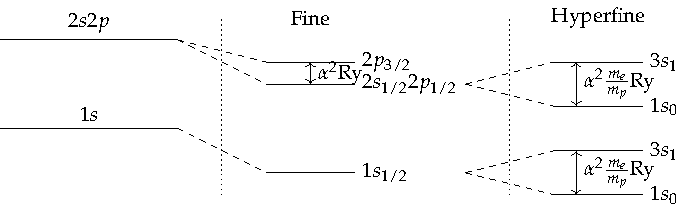
\includegraphics[]{Images/fig-hyperfinestructuresplit.pdf}

    \caption{Splitting in hydrogen atom energy levels due to the fine structure and hyperfine structure. Figure is not to scale (the hyperfine splittings are $\sim 10^{-3}$ smaller compared to the fine structure). Note the hyperfine splitting only occurs for the $s$ states (as it only occurs for states whose radial wavefunction is nonvanishing at the origin) and the split is between the singlet and triplet states. The $3/1$ denotes triplet/singlet and the $1/0$ denotes the total joint spin as $1$ or $0$.}
    \label{fig-hyperfinestructuresplit}
\end{figure}

However note that thus far we have only discussed internal fields. We today discuss external ones.

\subsection{Stark Effect - Large Field}
We consider a hydrogen atom in the presence of an electric field (in particular oriented in the $z$ direction). This has the corresponding Hamiltonian:
\begin{equation}
    H^{(1)} = -\v{d} \cdot \v{E}^{ext} = -ezE_z^{ext}
\end{equation}
We now ask what the typical scale of this perturbation is. $z \sim a_B$, so it is of scale $e a_B E_{ext}$. We consider the limit where the external field is much stronger than the fine structure corrections:
\begin{equation}
    e a_B E^{ext} \gg \alpha^2 \si{Ry} \sim 10^{-5} 10 \si{eV}
\end{equation}
and so:
\begin{equation}
    E^{ext} \gg \frac{ 10^{-5} 10 \si{eV}}{\abs{e}10^{-8}\si{m}} \sim 10^{4}\si{V.cm^{-1}}.
\end{equation}

Are fields of such magnitude present in nature? Certainly; consider a thunderstorm. Lab-wise, the largest field we can achieve is $100\si{MeV.m^{-1}}$, or $10^{6}\si{V.cm^{-1}}$ in linear accelerators. We discuss this large field limit, so we can do perturbation theory not with the fine structure states but with the unperturbed hydrogen atom states $\ket{n, l}$. We consider:
\begin{equation}
    \bra{n=1, l=0}H^{(1)}\ket{n=1,l=0} = 0
\end{equation}
This can be seen from the fact that $H' \propto z$, and then using that $\ket{n=1, l=0}$ are eigenstates of parity (with eigenvalue $1$), by symmetry we see that:
\begin{equation}\label{eq-paritymatelezero}
    \begin{split}
        \bra{n=1, l=0}H^{(1)}\ket{n=1, l=0} &\propto \bra{n=1, l=0}z\ket{n=1, l=0} 
        \\ &= \bra{n=1, l=0}\Pi^\dag z \Pi \ket{n=1, l=0} 
        \\ &= \bra{n=1, l=0}(-1)z \ket{n=1, l=0} 
        \\ &= -\bra{n=1, l=0}z\ket{n=1, l=0}
    \end{split}
\end{equation}
and so the matrix element must vanish. In calculating the energy correction, we have degeneracy and thus must use degenerate PT. To this end it is useful to consider what the good quantum numbers are. First, we see that:
\begin{equation}
    [L_z, H^{(1)}] = 0
\end{equation}
as $H^{(1)} \propto z$. However:
\begin{equation}
    [\v{L}^2, H^{(1)}] \neq 0
\end{equation}
as we do not have a general rotational symmetry here, only a symmetry for rotations about $z$.

In particular, let us consider the $n = 2$ states of hydrogen There are four degenerate states:
\begin{itemize}
    \item $\ket{n=2, l=0, m=0}$
    \item $\ket{n=2, l=1, m=0}$
    \item $\ket{n=2, l=1, m=1}$
    \item $\ket{n=2, l=1, m=-1}$
\end{itemize}
We now consider the matrix $T_{ab}$ of matrix elements of $H^{(1)}$ with the above states. But we find that all but two numbers vanish:
\begin{equation}
    T_{ab} = \m{0 & \cdot & 0 & 0 \\ \cdot & 0 & 0 & 0 \\ 0 & 0 & 0 & 0 \\ 0 & 0 & 0 & 0}
\end{equation}
and in particular we only need to compute one by Hermicity. How to see this? First, since $m$ is a good quantum number, only matrix elements with the same $m$ are nonzero. Second, only eigenstates of different parities will have a nonzero matrix element; else we could repeat the argument in Eq. \eqref{eq-paritymatelezero} to conclude that these matrix elements vanish. In other words, only matrix elements with the same $m$ and $l$s of different parity (actually more specifically $\delta l = \pm 1$) will be nonvanishing. Therefore the only matrix element to compute is:
\begin{equation}
    \begin{split}
        T_{12} &= \bra{n=2, l=1, m=0}-erE\cos\theta \ket{n=2, l=0, m=0}
        \\ &= -e\int R_{20} r R_{21} r^2 dr \int Y^0_0 \cos\theta Y_1^1 d\Omega
        \\ &= 3eaE^{ext}
    \end{split}
\end{equation}
so:
\begin{equation}
    T_{ab} = 3eaE^{ext}\m{0 & 1 & 0 & 0 \\ 1 & 0 & 0 & 0 \\ 0 & 0 & 0 & 0 \\ 0 & 0 & 0 & 0}
\end{equation}
So our computation reduces to:
\begin{equation}
    \det(T_{ab} - \delta_{ab}E^{(1)}) = \det\m{-E^{(1)} & 3eaE \\ 3eaE & -E^{(1)}} = 0
\end{equation}
we hence obtain:
\begin{equation}
    E^{(1)}_\pm = \pm 3eaE
\end{equation}
These have corresponding eigenvectors:
\begin{equation}
    \v{v}_+ = \frac{1}{\sqrt{2}}\m{1\\1}, \quad \v{v}_- = \frac{1}{\sqrt{2}}\m{1\\-1}
\end{equation}
So therefore the superpositions of interest are:
\begin{equation}
    \psi_\pm = \frac{1}{\sqrt{2}}\left(\ket{n=2, l=1, m=0} \pm \ket{n=2, l=0, m=0}\right)
\end{equation}
with energies:
\begin{equation}
    E = E_0 \pm E^{(1)} =  -\frac{1}{4}\si{Ry} \pm 3eaE 
\end{equation}
Graphically, we have the spectrum:
\begin{figure}[htbp]
    \centering
    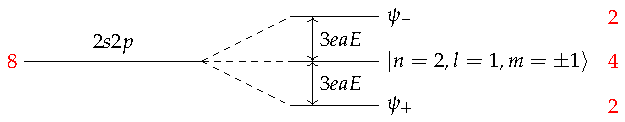
\includegraphics[]{Images/fig-strongstarkeffectsplit.pdf}
    
    \caption{(Linear) Stark Effect splitting of the 8-fold degenerate $2s2p$ energy level in the Hydrogen atom in the presence of a strong external electric field. The energy level splits into three levels, separated by $3eaE$. The degeneracies of the new levels are denoted in red.}
    \label{fig-strongstarkeffectsplit}
\end{figure}

We still have the degeneracy from the spin (although it does not factor into the problem here), and one of the levels remains without a change in the energy. Note that if we included fine structure on top of this, we would have a further splitting in the above diagram (but of a much smaller order of magnitude than the E-field splitting). Note also that if the electric field perturbation was on the same order of magnitude as the fine structure perturbation, then we would consider the perturbing Hamiltonian to be the sum of the E-field and fine structure terms, and we would have to diagonalize a much less simple $T_{ab}$ matrix.

\subsection{Stark Effect - Small Field}
We now consider an electric field that is small on the scale of the fine structure corrections. We apply the perturbations onto the fine structure corrected states. The $1s_{1/2}$ state remains unaffected (there is no correction from the electric field here, independent of the field strength - all states have the same parity of $l = 0$ here so there cannot be any correction).

There is also no splitting for the $2p_{3/2}$ as all of the matrix elements would be zero. Again, the same parity argument; all four states here have $l = 1$ and so the matrix elements vanish.

The only level which exhibits splitting is the $2s_{1/2}2p_{1/2}$ level as there can be nonzero matrix elements between the $l = 1$ and $l = 0$ states. In particular we obtain (without going through the entire calculation again):
\begin{equation}
    \ket{\psi_\pm} = \frac{1}{\sqrt{2}}\left(\ket{l=1, m=0, s_z = \frac{1}{2}} \pm \ket{l=1, m=1, s_z = -\frac{1}{2}}\right)
\end{equation}
(Ok, this was not so clear to me here how the above formula follows, but oh well). The energy splitting can be seen in Fig.

\begin{figure}[htbp]
    \centering
    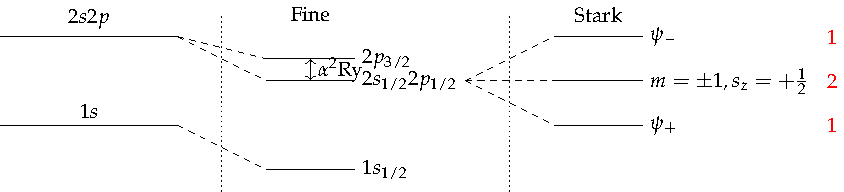
\includegraphics[]{Images/fig-weakstarkeffectsplit.pdf}
    
    \caption{Stark effect splitting of the $2s_{1/2}2p_{1/2}$ (fine structure) energy level due to a weak external electric field. The fourfold degenerate level splits into three levels.}
    \label{fig-weakstarkeffectsplit}
\end{figure}

\subsection{Selection Rules - Calculating expectation values of z}
Let us consider a general matrix element:
\begin{equation}
    \bra{n'l'm'}z\ket{nlm}
\end{equation}
Since $[L_z, z] = 0$, we have:
\begin{equation}
    \bra{n'l'm'}L_z z - zL_z\ket{nlm} = 0 \implies (m' - m)\bra{l'm'}z\ket{lm} = 0
\end{equation}
and so if $m \neq m'$ then the matrix element must vanish. So we obtain the selection rule that $m = m'$. 

Now, we consider the selection rule based on $l$. We will find that $\Delta l = \pm 1$ must be enforced for the matrix element must be zero (the parity argument we make previously only establishes that the $l$s must be of different parity; this is a stronger condition). There is an argument from Clebsch-Gordon coefficients that can show this condition to be true.

\subsection{Zeeman Effect}
We consider an external magnetic field, giving rise to a perturbing Hamiltonian:
\begin{equation}
    H^{(1)} = -\gv{\mu} \cdot \v{B}^{ext}, \quad \gv{\mu}\frac{-\abs{e}\hbar}{2mc}\left(\v{L} + 2\v{S}\right)
\end{equation}
Numerically:
\begin{equation}
    \frac{\abs{e}\hbar}{2mc} = 5.8 \times 10^{-9}\si{eVG^{-1}}
\end{equation}
(we igonore the proton; its contribution is supressed by 2000 or so). We have a strong Zeeman effect when:
\begin{equation}
    \mu B^{ext} \gg \alpha^2 \si{Ry}
\end{equation}
or when:
\begin{equation}
    B^{ext} \gg \frac{10^{-5}10\si{eV}}{10 10^{-9} \si{eV}} G = 10^4 \si{G} = 1\si{T}
\end{equation}
so if the external B-field is much larger than a Tesla, then we have a strong-field Zeeman effect (and weak-field Zeeman effect if much less than a Tesla). 

For scales, MRI/NMR is on the order of Tesla, the LHC is on the order of 10 Tesla, and Earth's B-field is on the order of half a Gauss.

Looking at the commutation relations, we have:
\begin{equation}
    [H', \v{L}^2] = [H', L_z] = [H', \v{S}^2] = [H', \v{S}^2] = 0
\end{equation}
as is clear from looking at the Hamiltonian. We can do the whole matrix elements, and it will be a simple matter of:
\begin{equation}
    \Delta E = \bra{\cdot}2S_z + L_z\ket{*} \frac{-\abs{e}\hbar}{2mc}
\end{equation}
and this is trivial as of course the states are eigenstates of $L^2, S^2, L_z, S_z$! The energy splitting from the (strong-field) Zeeman effect therefore looks as in Fig. 

\begin{figure}[htbp]
    \centering
    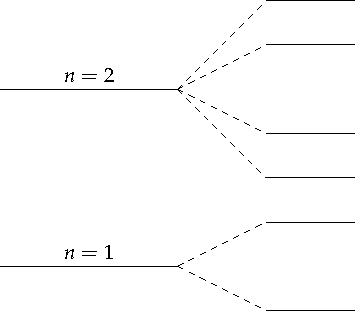
\includegraphics[]{Images/fig-strongzeemaneffectsplit.pdf}

    \caption{Energy splitting of the hydrogen atom levels from the strong-field Zeeman effect.}
    \label{fig-strongzeemaneffectsplit}
\end{figure}

This correction becomes less trivial when the magnetic field is weaker (as we need to take into account the fine structure... and so our states we use are no longer eigenstates of $L^2, S^2, L_z, S_z$); but we can still do the calculation of the matrix elements above. It will be convenient to write it as $\bra{\cdot}J_z + S_z\ket{\cdot}$ instead.

The last question of the HW asks for considerin the interplay of fine hyperfine, and zeeman effects in the Hydrogen atom; have fun! We start WKB next week.
\newpage
\section{The WKB Approximation}
The WKB, or Wentzel-Kramers-Brillouin, or semiclassical, or quasiclassical approximation, or the method of steepest descent (used often by mathematicians to find asymptotic behavior of functions in complex analysis!)

\subsection{Motivation for Approximations}
We have three cases in QM where the particle can be solved exactly; the free particle ($V = 0$), the quantum harmonic oscillator ($V = \frac{kx^2}{2}$), and the hydrogen atom ($V = \frac{e^2}{r}$). So in order to study nature, we have to develop the study of approximations. 

We have already studied time-independent perturbation theory. This has applications such as the fine/hyperfine structures of Hydrogen and the Stark/Zeeman effects. The basis idea is that we have some perturbation $V$ much smaller than the typical energy scale of the problem, $\abs{V} \ll \abs{E_n - E_m}$. We then solve for the lowest-order corrections to the energy coming from this small perturbation.

However, this has a problem. Consider for example the Stark effect, where we had the Hamiltonian:
\begin{equation}
    H = -\frac{e^2}{r} - eEz
\end{equation}

\begin{figure}[htbp]
    \centering
    \textcolor{blue}{TODO: Potential profile for stark effect}
    \caption{<caption>}
    \label{<label>}
\end{figure}
where we treated $-\frac{e^2}{r}$ as the primary Hamiltonian and $-eEz$ as the perturbation. However, consider the phenomena of ionization, where the electric field ionizes hydrogen atoms, freeing the electron. The question: how do we see this phenomena arise in the perturbation theory calculation? We calculate some series $\sum_n c_n g^n$; but no matter to what order we calculate, we don't see the phenomena of ionization. What is the problem? There are some functions which are non-analytic; e.g. $\exp(-\frac{1}{g})$ which cannot be recovered in perturbation theory (as a series expansion of these functions are not meaningful). There are many crucial phenomena attached to this, e.g. ionization, tunneling, alpha decay and so on.

A side note: note that $m_p \sim e^{-1/g}$ - baryonic mass is non-perturbative. So people who use QCD have trouble understanding this phenomena as perturbation theory is pretty useless here.

\subsubsection{Motivation for WKB}
WKB is suited to describe such phenomena. In fact, the potential $V$ is allowed to be large here. The condition we impose is that the potential is slowly varying:
\begin{equation}
    \abs{\dpd{V}{x}} \ll 1
\end{equation}
We discuss phenomena such as ionization, tunneling, (classically describable) highly excited states\footnote{Highly excited states are closer to classical states than the ground states of QM systems.}, which have non-analytic behavior $\exp(-\frac{1}{V})$ which cannot be treated in perturbation theory. 

\subsubsection{Motivation for Adiabatic (Born-Oppenheimer) Approximation}
We consider this approximation when we have slow and fast degrees of freedom. This is often useful for molecular physics. Here we have many nuclei and many electrons. The electron degrees of freedom are extremely fast, with typical frequencies being the electron degrees of freedoms. Comparatively, the protons move very slowly. We can see this as $\frac{m}{M} \ll 1$. It is often used in molecular physics, particle physics and condensed matter physics. The potential can be large, but the key is that there are degrees of freedom moving at different speeds.

\subsubsection{Motivation to Time-Independent PT}
This is useful for treating problems such as radiation and scattering. It is closely related to path integrals in QM, geometric phases, and topological effects. 

\subsection{WKB in 1D}
We have the Schrodinger equation:
\begin{equation}
    -\frac{\hbar^2}{2m}\dod[2]{\psi}{x} + U(x)\psi = E\psi
\end{equation}
if $U \sim \text{Const.}$, then the solutions are known:
\begin{equation}
    \psi \sim e^{\pm i\frac{px}{\hbar}}
\end{equation}
with $\frac{p^2}{2m} = E - U$. We do a change of variables now to write:
\begin{equation}
    \psi(x) = e^{i\frac{S(x)}{\hbar}}
\end{equation}
The logic when developing WKB was that the action $S$ was large for classical physics. Anyways, let us write down what $\psi', \psi''$ are:
\begin{equation}
    \psi' = e^{i\frac{S}{\hbar}}\left(i\frac{S'}{\hbar}\right)
\end{equation}
\begin{equation}
    \psi'' = e^{i\frac{S}{\hbar}}\left(i\frac{S'}{\hbar}\right)^2 + i\frac{S''}{\hbar}e^{i\frac{S}{\hbar}}
\end{equation}
Now let's substitute this back into the SE. No approximations have been made yet here. We're just substituting in an Ansatz:
\begin{equation}
    -\frac{\hbar^2}{2m}\left(-\frac{S'^2}{\hbar^2}\right) - \frac{\hbar^2}{2m}\left(i\frac{S''}{\hbar}\right) + U - E = 0
\end{equation}
now we consider the expansion (which is possible as $S$ is analytic so long as the potential is smooth - but this is quite a deep question. We'll assume the analyticity):
\begin{equation}
    S = S^{(0)} + \frac{\hbar}{i}S^{(1)} + \left(\frac{\hbar}{i}\right)^2S^{(2)} + \ldots
\end{equation}
now, the $S^{(0)}$ in the above is assumed to describe the (large) classical part. We substitute in our expansion and collect terms in various powers of $\hbar$:
\begin{equation}
    -\frac{1}{2m}\left((S^{(0)})'\right)^2 + \frac{i\hbar}{2m}(S^{(0)})'' + E - U - \frac{2}{2m}(S^{(0)})' \frac{\hbar}{i}(S^{(1)})'
\end{equation}
The terms to order $\hbar^0$ give us:
\begin{equation}
    [(S^{(0)})']^2 = 2m(E - U)
\end{equation}
And the terms to order $\hbar^1$ give us:
\begin{equation}
    \frac{i\hbar}{2m}\left[(S^{(0)})'' + 2(S^{(0)})'(S^{(1)})'\right] = 0
\end{equation}
We can rearrange the order $\hbar^0$ equation to obtain:
\begin{equation}
    (S^{(0)})' = \pm \sqrt{2m(E - U)}
\end{equation}
note $p^2/2m = E - U$, and we therefore obtain:
\begin{equation}
    S^{(0)} = \pm \int_0^x p(x') dx'.
\end{equation} 
So we have successfully generalized our formula for the free particle $\psi(x) = e^{\pm i \frac{px}{\hbar}}$. We can see that when $p(x) = p$ a constant that the above formula reproduces the free particle result. So, we have our first result:
\begin{equation}
    \psi(x) = e^{i\frac{S(x)}{\hbar}} = e^{\pm\frac{i}{\hbar}\int_0^x p(x')dx'}
\end{equation}
We can now calculate $S^{(1)}$ using the second equation:
\begin{equation}
    (S^{(0)})'' = - 2(S^{(0)})'(S^{(1)})'
\end{equation}
since $(S^{(0)})' = \pm p(x)$ and $(S^{(0)})'' = \pm \od{p}{x}$, we find:
\begin{equation}
    (S^{(1)})'  -\frac{(S^{(0)})''}{2(S^{(0)})'} = -\dod{p}{x}\frac{1}{2}\frac{1}{p} = -\frac{1}{2}\dod{\log p}{x}
\end{equation}
Therefore:
\begin{equation}
    S^{(1)} = -\frac{1}{2}\log p(x)
\end{equation}
Therefore:
\begin{equation}
    \psi = e^{i\frac{S^{(0)} - i\hbar S^{(1)}}{\hbar}} = e^{\pm i \int^x \frac{p(x')dx'}{\hbar}}\frac{1}{\sqrt{p(x)}}
\end{equation}
If we look at $\abs{\psi}^2$, we have:
\begin{equation}
    \abs{\psi}^2 \sim \frac{1}{\abs{p(x)}} = \frac{1}{mV(x)}
\end{equation}
if we ask the probability of finding a particle, then:
\begin{equation}
    \abs{\psi^2}dx = \frac{dx}{V(x)} = dt
\end{equation}
If we describe the classical physics for a particle in an oscillator, the particle spends a lot of time near the turning points where the velocity is lowest and not a lot of time in the minimum where the velocity is the highest. We reproduce the classical result! WKB were very happy with this.

We have to ask when this approximation is valid. We have the condition assuming:
\begin{equation}
    \abs{\hbar S^{(1)}}' \ll \abs{(S^{(0)})'}
\end{equation}
and so:
\begin{equation}
    \abs{\frac{1}{2}\dod{p}{x}\frac{\hbar}{p}} \ll \abs{p}
\end{equation}
and so:
\begin{equation}
    \dod{}{x}\left(\frac{\hbar}{p}\right) \ll \abs{\dod{\lambda}{x}} \ll 1
\end{equation}
so our approximation is justified when the wavelength of the particle varies slowly with distance.

\newpage
\section{WKB Continued}
\subsection{A review of WKB motivation and derivation}
The basic idea of WKB is the following. What we want to do is to find some approximation where we can study effects that cannot be revealed using perturbation theory. Many functions can be expanded in a series $\sum_n c_n g^n$, but not all effects can be computed; namely those that go as $e^{-\frac{1}{g}}$ (as all derivatives of these classes of functions vanish). So, we want to study a different type of approximation to PT which allows us to probe such functions.

Our WKB approximation tells us that the wavefunction has the approximate form:
\begin{equation}
    \psi(x) \sim e^{\pm i \int^x \frac{p(x')dx'}{\hbar}} \frac{1}{\sqrt{\abs{p(x)}}}
\end{equation}
The way we did our expansion is justified so long as:
\begin{equation}
    \dod{}{x}\left(\frac{\hbar}{p(x)}\right) \ll 1 \implies \left| \dod{\lambda}{x}\right| \ll 1
\end{equation}

\subsection{When does WKB hold?}
We take $p(x) = \sqrt{2m(E - U(x))}$ and so:
\begin{equation}
    \dod{}{x}\left(\frac{\hbar}{p(x)}\right) \ll 1 \implies \dod{}{x}\left(\frac{\hbar}{\sqrt{2m(E - U(x))}}\right) \ll 1
\end{equation}
so then:
\begin{equation}
    \left|\frac{\hbar}{\sqrt{2}m}\frac{1}{(E - U)^{3/2}}\frac{1}{2}\dod{U}{x}\right| \ll 1
\end{equation}
If $E \gg U$ then:
\begin{equation}
    \left|\frac{\hbar}{\sqrt{2}m}\frac{1}{E^{3/2}}\frac{1}{2}\dod{U}{x}\right| \ll 1
\end{equation}
So for excited enough states, this approximation is always justified (e.g. the Harmonic oscillator has $E \sim n$, so for $n$ sufficiently large the LHS is small).

\begin{figure}[htpb]
    \centering

    \caption{}
    \label{}
\end{figure}

However, we also see places where the approximation is never justified; in particular, for $E \sim U$ (the turning points) the LHS explodes and so the condition is not satisfied.

Note we have been assuming $\od{U}{x} \sim 1$ throughout.

\subsection{A simple example}
We consider some smooth potential profile $U(x)$ in an infinite square well. 

\begin{figure}[htbp]
    \centering
    \begin{tikzpicture}[scale=1]
        \filldraw[color=gray!30, fill=gray!30] (0, 0) -- (-2, 0) -- (-2, 3.5) -- (0, 3.5) -- cycle;
        \filldraw[color=gray!30, fill=gray!30] (3, 0) -- (3, 3.5) -- (5, 3.5) -- (5, 0) -- cycle;
        \draw[latex-latex, thick] (-2, 0) -- (5, 0);
        \draw[-latex, thick] (0, 0) -- (0, 3.5);
        \draw[-latex, thick] (3, 0) -- (3, 3.5);
        \node[below] at (0, 0) {$x = 0$};
        \node[below] at (3, -0.1) {$x = a$};
        \node[above] at (-1, 1.75) {$U = \infty$};
        \node[above] at (4, 1.75) {$U = \infty$};
        \draw [thick] (0, 2) to [ curve through ={(0.25, 1.95) ..(0.5,1.75) .. (0.75, 1.65)   . . (1, 1.6) . . (1.5,1.375) . . (1.75, 1.5) ..  (2, 1.45) .. (2.5,1.65) .. (2.75, 1.75).. }] (3,2);
        \node[] at (1.5, 1.8) {$U(x)$};
    \end{tikzpicture}
    \caption{<caption>}
    \label{<label>}
\end{figure}

We have that:
\begin{equation}
    \psi_\pm (x) = e^{\pm i\phi(x)}
\end{equation}
where:
\begin{equation}
    \phi(x) = \int_0^x \frac{p(x')dx'}{\hbar}
\end{equation}
as usual:
\begin{equation}
    p^2 = 2m(E - U)
\end{equation}
taking a superposition of the solutions, we have:
\begin{equation}
    \Psi(x) = \psi_+(x) + \psi_-(x) = \frac{A_+}{\sqrt{p}}\cos(\phi(x)) + \frac{A_-}{\sqrt{p}}\sin(\phi(x))
\end{equation}
But by the boundary conditions, $\Psi(0) = 0$ and so since $\phi(0) = 0$ we find that $A_+ = 0$. Then, since we also have that $\Psi(a) = 0$ and so from $\sin(\phi(a)) = 0$ we find that $\phi(a) = n\pi$. Therefore:
\begin{equation}
    \int_0^a \frac{p(x')dx'}{\hbar} = \pi n
\end{equation}
Note in the special case where $U(x) = 0$, we can carry out the integral explicitly  and find:
\begin{equation}
    \frac{pa}{\hbar} = \pi n
\end{equation}
and solving for the energies:
\begin{equation}
    E_n = \frac{\hbar n^2\pi^2}{2ma^2}
\end{equation}
which is exactly the result we got from doing it analytically in our first QM class.

We can agai

\textcolor{blue}{TODO: Validity of WKB SOLUTIONS - study the same way as 14.2}

\subsection{Connection Formulae - Motivation and Setup}
We now study the turning points. Consider the following:

\textcolor{blue}{TODO: diagram}


In the classically forbidden region (with $E < U(x)$) we can do exactly the same computations as we did for the classically allowed region; the only difference is now:
\begin{equation}
    \frac{p^2}{2m} = E - U(x)
\end{equation}
And so we obtain different WKB solutions:
\begin{equation}
    \frac{1}{\abs{p}}e^{\pm i \int^x \frac{p(x')dx'}{\hbar}} \to \frac{1}{\abs{p}}e^{\pm \int \frac{p(x')dx'}{\hbar}}
\end{equation}
where the left formula is for the classically allowed region, with $p^2/2m = E - U$ and the right formula is for the classically forbidden region with $p^2/2m = U - E$ (the exact same analysis from last class applies to study this region). In the classically forbidden region, we have:
\begin{equation}
    \Psi_2(x) = \frac{D}{\sqrt{p}}e^{-\int_0^x \frac{p(x')dx'}{\hbar}}
\end{equation}
where $p^2 = 2m(U-E)$. Note that we \emph{only} consider the negative exponential solution; our wavefunctions must be normalizable and hence we throw away the $\sim \exp(+x)$ solution that is non-normalizable as $x \to \infty$.

So, we understand that far away from the turning point to the left (the classically allowed region) we have $e^{\pm i \int^x \frac{p(x')dx'}{\hbar}}$ solutions and far away from the turning point going to the right (the classically forbidden region) we have $e^{-\int_0^x \frac{p(x')dx'}{\hbar}}$ solutions. But what happens near the turning point? We discuss this now.

How do we do this? Many textbooks consider the linear potential near the turning point, which has known solutions of Airy functions. Far away to the left we find WKB sinusoidal solutions and far away to the right we have WKB exponential decay solutions. The Airy function is analytical and has the correct limits going away from the turning point. It is therefore a solution, and this is precisely what the connection formulae are. This is a very long derivation!

We go through this problem slightly differently. We recall that WKB does not apply at the turning point; our wavefunction is straightly wrong. We take $x \to z$ the complex plane. We then analytically continue our wavefunction, and obtain the connection formulae this way.

\subsection{Connection Formulae from Analytic Continuation}
We write down the superposition for $\psi_1$ (in the classically allowed region) in the following way. We have:
\begin{equation}
    \psi_1(x) = \left(\frac{B}{\sqrt{p(x)}}e^{+i\int_x^0 \frac{p(x')dx'}{\hbar}} + \frac{C}{\sqrt{p(x)}}e^{-i\int_x^0 \frac{p(x')dx'}{\hbar}}\right)
\end{equation}
We consider Taylor expanding the potential:
\begin{equation}
    U = U(0) + U'(0) x' = U_0 + U_0' x'
\end{equation}
such that now:
\begin{equation}
   \int  p(x)' dx' = \int x^{1/2}dx'\sqrt{2mU_0'}
\end{equation}
We now go to the complex plane. We write $x' = \rho e^{i\phi}$. We will do the integral and then do analytical continuation from $\phi = 0$ to $\phi = \pi$. Why can I do this? In the complex plane I can think that I can meander around the pole $E = U$ (compare to the real axis; we can't avoid the pole), so we don't hit it.

We carry out:
\begin{equation}
    \int_0^x \sqrt{x'}dx' = \frac{2}{3}\rho^{3/2}e^{i\frac{3}{2}\phi} = \begin{cases}
        \frac{2}{3}\rho^{3/2} & \phi = 0
        \\ \frac{2}{3}\rho^{3/2}e^{i\frac{3\pi}{2}} = -i\frac{2}{3}\rho^{3/2} & \phi = \pi
    \end{cases}
\end{equation}
We have thus ``collected the phase'' in the integral in the correct way. There is another term to consider; namely the $\frac{1}{\sqrt{p}}$. This collects a phase:
\begin{equation}
    \frac{1}{\sqrt{p}} \to \frac{1}{\sqrt{p}e^{i\pi/4}}
\end{equation}
When we analytically continue the classically forbidden region solution to the classically forbidden region, we obtian:
\begin{equation}
   \psi_2(x) = \frac{D}{\sqrt{p}}e^{-\int_0^x \frac{p(x')dx'}{\hbar}} \to \frac{D}{\sqrt{p}}e^{+i\int_x^0 \frac{p(x')dx'}{\hbar} - \frac{i\pi}{4}}
\end{equation}
For the other $e^{-i\ldots}$ term, we analytically contnue in the other direction, going from $\phi = 0$ to $\phi = -\pi$. So, we can write down $\psi_1$ as:
\begin{equation}
    \psi_1(x) = \frac{2D}{\sqrt{p}}\left(\cos(\int_x^0 \frac{p(x')dx'}{hbar} - \frac{\pi}{4})\right)
\end{equation}
where the cosine is obtained via the superposition of the two terms. We can write this equivalently as:
\begin{equation}
    \psi_1(x) = \frac{2D}{\sqrt{p}}\left(\sin(\int_x^0 \frac{p(x')dx'}{\hbar} + \frac{\pi}{4})\right)
\end{equation}
and the claim is the following: $\psi_2$ in classically forbidden region corresponds to this $\sin$, which is the superposition of the two plane waves in the classically allowed region, with the exact same coefficients.
\newpage
\section{WKB Part III}

\subsection{Review of the Connection Formula Derivation}
Let us explain what we have derived. Let assume a setup as in Fig. \ref{fig-connectionformula}. The wavefunction in the neighbourhood around the turning point $U = E$ (let us call this point $x_2$) cannot be described by WKB. But if $\psi_2$ (in the calssically forbidden region) is described by the form:
\begin{equation}
    \psi_2(x) = \frac{D}{\sqrt{p}}e^{-\frac{1}{\hbar}\int_{x_2}^x p(x')dx'}
\end{equation}
then $\psi_1(x)$ in the classically allowed region has the structure:
\begin{equation}
    \psi_1(x) = \frac{2D}{\sqrt{p}}\sin\left(\frac{1}{\hbar}\int_{x}^{x_2} p(x')dx' + \frac{\pi}{4}\right)
\end{equation}

Let us make a simple point; the fact that a sine appears in the above is absolutely trivial; we have imaginary exponential solutions to the SE in the classically allowed region. The nontrivial part is the $+\frac{\pi}{4}$ phase appears.

\subsection{Deriving the Bohr-Sommerfield Quantization Formula}
We can repeat exactly the same arguments for a setup like Fig. \ref{fig-connectionformula} but with the classically forbidden region to the left and the classically allowed region to the right of a turning point $x_1$. We then have that $\psi(x)$ to the left of the turning point is:
\begin{equation}
    \psi_{x < x_1}(x) = \frac{D'}{\sqrt{p}}e^{-\frac{1}{\hbar}\int_x^{x_1} p(x')dx'}
\end{equation}
note the order of the integral which ensures the decay of the wavefunction at infinity. We get an extremely similar formula for the wavefunction in the classically allowed region:
\begin{equation}
    \psi_{x > x_1}(x) = \frac{2D'}{\sqrt{p}}\sin\left(\frac{1}{\hbar}\int_{x_1}^{x} p(x')dx' + \frac{\pi}{4}\right)
\end{equation}

We now present a non-trivial claim: We claim that we can use the connection formulas going from both sides (assume we have $U$ which such that $x_1 < x < x_2$ is a classically allowed region inside $x_1 > x$ and $x > x_2$ are classically forbidden). When we do this, the wavefunctions inside of the classically allowed region \emph{must agree}. We therefore obtain the condition:
\begin{equation}
    \sin\left(\frac{1}{\hbar}\int_{x_1}^{x} p(x')dx' + \frac{\pi}{4}\right) = \pm \sin\left(\frac{1}{\hbar}\int_{x}^{x_2} p(x')dx' + \frac{\pi}{4}\right)
\end{equation}
where the $\pm$ comes from $D' = \pm D$. We now consider writing the integral on the LHS as:
\begin{equation}
    \int_{x_1}^x + \frac{\pi}{4} = \int_{x_2}^x  + \int_{x_1}^{x_2} + \frac{\pi}{4} = -\int_{x}^{x_2} + \int_{x_1}^{x_2} + \frac{\pi}{4} - \frac{\pi}{4} + \frac{\pi}{4}
\end{equation}
We then see that $-\int_{x}^{x_2} - \frac{\pi}{4}$ precisely appears on the RHS, and so we obtain the \emph{Bohr-Sommerfield quantization condition}:
\begin{equation}
    \theta = \int_{x_1}^{x_2} + \frac{\pi}{2} = n\pi
\end{equation}
or rewriting this:
\begin{equation}
    \boxed{\int_{x_1}^{x_2}\frac{p(x')dx'}{\hbar} = \pi(n + \frac{1}{2})}
\end{equation}

\subsection{Analyzing the Bohr-Sommerfield Quantization Formula}
\begin{enumerate}[(a)]
    \item What is $n$? This is the number of nodes inside the potential, or also the excitation number.
    \item We can reformulate the condition as:
    \begin{equation}
        n = \int_{x_1}^{x_2}\frac{pdx}{\hbar \pi} = \oiint_{\frac{P^2}{2m} \leq E - U} \frac{dpdx}{2\pi\hbar} = \oint \frac{pdx}{2\pi\hbar}
    \end{equation}
    So what does this say? We take the phase volume of the system, and divide this by $2\pi\hbar$; We therefore obtain the nuber of quantum cells! 
    \item We find that one quantum cell has volume $2\pi\hbar$ (this could also follow by considering the uncertainty relation).
    \item In $3D$, we can generalize everything we have just said, and write:
    \begin{equation}
        dn = \frac{d^3pd^3x}{(2\pi\hbar)^3} = \frac{V}{(2\pi\hbar)^3}p^2dpd\Omega
    \end{equation}
    Often we can represent $p$ in terms of energy, and find the number of states per unit energy (density of states in terms of energy). Explicitly, we can see that $p^2 dp = pEdp$ which follows from:
    \begin{equation}
        E^2 = p^2  +m^2 \implies EdE = pdp
    \end{equation}
    This is correct for both nonrelativistic and relativistic physics (we will use this formula to study photons). For free particles with $E = p^2/2m$, we find:
    \begin{equation}
        \frac{1}{V}\frac{dn}{dE} = \frac{d\Omega}{(2\pi\hbar)^3}\abs{p}E
    \end{equation}
    which is the number of states per unit energy per unit volume. Density of states is extremely useful, and comes up in many places in physics, such as:
    \begin{itemize}
        \item Fermi liquid model in condensed matter physics
        \item Transitions in atomic physics
        \item Thomas-Fermi models for complex models.
    \end{itemize}
\end{enumerate}

\subsection{Solving the QHO with WKB}
Let us use WKB to solve the simplest problem there is; the Harmonic Oscillator. We want to quantize it assuming we don't know the exact solution. Writing down the Bohr-Sommerfield quantization condition, we find:
\begin{equation}
    \int_{-a}^a pdx = \pi\hbar(n + \frac{1}{2})
\end{equation}
We have $p = \sqrt{2m(E - U(x))}$ and $U(x) = \frac{1}{2}kx^2$. At $x = \pm a$ we have $E = \frac{ka^2}{2}$ and so:
\begin{equation}
    \int_{-a}^{a} pdx = a\sqrt{2mE}\int_{-a}^{a}\sqrt{1 - \left(\frac{x}{a}\right)^2}\frac{dx}{a}
\end{equation}
Now making the substitution $z = \frac{x}{a}$ with $z \in (-1, 1)$, we can evaluate the integral (e.g. via trigonometric substitution) to find:
\begin{equation}
    \int_{-a}^{a} pdx  = \sqrt{\frac{2E}{k}}\sqrt{2mE}\frac{\pi}{2} = \pi\hbar(n + \frac{1}{2})
\end{equation}
With $\omega^2 = k/m$, we find:
\begin{equation}
    E = \hbar\omega(n + \frac{1}{2})
\end{equation}
and we reproduce exactly the analytical result for the eigenenergies of the oscillator! Nevertheless, we cannot trust this result for sufficiently small $n$. How do we find out when this formula can be trusted? We go back to the discussion of when WKB is justified:
\begin{equation}
    \left|\dod{}{x}\frac{\hbar}{p}\right| \ll 1
\end{equation}
Differentiating, we find:
\begin{equation}
    \left|\frac{\hbar}{\sqrt{2m}}\frac{1}{(E - U)^{3/2}}\frac{1}{2}kx\right| \ll 1
\end{equation}
which with $U = \frac{1}{2}kx^2$, and $z = x/a$ becomes;
\begin{equation}
    \left| \frac{\hbar\omega}{E}\frac{z}{(1-z^2)^{3/2}}\right| \ll 1
\end{equation}
substituting in $E_n = \hbar\omega(n + \frac{1}{2})$ (and ignoring some coefficients) we have:
\begin{equation}
    \left|\frac{1}{(1-z^2)^{3/2}}\frac{1}{n}\right| \ll 1
\end{equation}
so for sufficiently large $n$, so long as we stay away from the turning points $z = \pm 1$ (i.e. $x = \pm a$) WKB is reliable here. How close we can get to the turning point will be a matter of how large $n$ is.

After the midterm on wednesday, we will use WKB to analyze tunnelling.
\newpage
\section{Midterm Review}

\subsection{Two Spin-1 Particles}
We consider a system made of two spin-1 particles with the Hamiltonian:
\begin{equation}
    H = \e_1 \v{S}^{(1)} \cdot \v{S} + \e_2(S_z)^2
\end{equation}
where $\v{S} = \v{S}^{(1)} + \v{S}^{(2)}$, $\e_1 > 0, \e_2 > 0$. 

\begin{enumerate}[(a)]
    \item Demonstrate (by computing the relevant commutators) that the classification $\ket{S^{(1)}, S^{(2)}, S, S_z}$ is a good classification scheme of states for this Hamiltonian.
    \item What is the lowest energy of the system?
    \item What is the ground state? Formulate your answer using the classification $\ket{S^{(1)}, S^{(2)}, S, S_z}$. Use CG coefficients to represent this state in terms of $\ket{S^{(1)}, S^{(2)}, S_z^{(1)}, S_z^{(2)}}$. 
    \item Compute the expectation value $\avg{S_x^{(1)}S_x^{(2)} + S_y^{(1)}S_y^{(2)}}$ for the ground state.
    \item \textbf{Strictly qualitative problem. No calculations!} What is the expectation value $\avg{S_z^{(1)}}$ for the ground state? Zero or nonzero? Present the arguments.
\end{enumerate}

\noindent
\textit{Solution.} 
\begin{enumerate}[(a)]
    \item We start by rewriting the Hamiltonian:
    \begin{equation}
        H = \e_1 (\v{S}^{(1)})^2 + \e_1\v{S}^{(1)} \cdot \v{S}^{(2)} + \e_2 (S_z)^2
    \end{equation}
    We can easily find that $[H, S^2] = 0$ and $[H, S_z] = 0$, $[H, (S^{(1)})^2] = [H, (S^{(2)})^2] = 0$ by writing $\v{S}^{(1)} \cdot \v{S}^{(2)} = \frac{1}{2}(S^2 - (\v{S}^{(1)})^2 - (\v{S}^{(2)})^2)$. Note that $[H, S_i] = 0$. 
    \item We rewrite:
    \begin{equation}
        H = \frac{\e_1}{2}\left(S_1^2 - S_2^2\right) + \frac{\e_1}{2}S^2 + \e_2 S_z^2
    \end{equation}
    $S_1^2 - S_2^2$ is invariant, so we pick a state such that $S^2, S_z^2$ are minimized. So we pick the state with $s = 0$ and $s_z = 0$. but then by symmetry $S_1^2 - S_2^2$ will be zero. So the ground state energy is zero.
    \item In the eigenbasis we have $\ket{s = 0, s_z = 0}$. We can use a CG table to write:
    \begin{equation}
        \ket{s = 0, s_z = 0} = \frac{1}{\sqrt{3}}\ket{s_z^{(1)} = -1, s_z^{(2)} = 1} + \frac{1}{\sqrt{3}}\ket{s_z^{(1)} = 0, s_z^{(2)} = 0} + \frac{1}{\sqrt{3}}\ket{s_z^{(1)} = 1, s_z^{(2)} = -1}.
    \end{equation}
    \item The easiest way to do this is to write:
    \begin{equation}
        \avg{S_x^{(1)}S_x^{(2)} + S_y^{(1)}S_y^{(2)}} = \avg{\v{S}^{(1)} \cdot \v{S}^{(2)} - S_z^{(1)}S_z^{(2)}}
    \end{equation}
    We then have:
    \begin{equation}
        \v{S}^{(1)} \cdot \v{S}^{(2)} = \frac{1}{2}(S^2 - (S^{(1)})^2 - (S^{(2)})^2)
    \end{equation}
    so computing the values using the relevant eigenbases:
    \begin{equation}
        \avg{S_x^{(1)}S_x^{(2)} + S_y^{(1)}S_y^{(2)}} = \frac{1}{2}(0 - 2 - 2) + \frac{2}{3} = -\frac{4}{3}
    \end{equation}
    \item $\avg{S_z^{(1)}} = 0$. Because a singlet is rotationally invariant, there is no preferred direction for a single spin.
\end{enumerate}


\subsection{Perturbation Theory for Two-Level System}
Cosnider a two-state system with a Hamiltonian represented in the spin $S_z$ basis as
\begin{equation}
    H^{(0)} = \m{a & 0 \\ 0 & b}.
\end{equation}
Now the system is perturbed with
\begin{equation}
    H' = \m{a_3 & a_1 \\ a_1 & -a_3}
\end{equation}
where $a_1 \approx a_3 \ll a, b$. 
\begin{enumerate}[(a)]
    \item Show that the unperturbed system described two levels with energies $E_1 = a$ and $E_2 = b$ correspondingly.
    \item Using first order perturbation theory to compute corrections to these energy levels.
    \item Compute the exact eigenenergies by diagonalizing the full Hamiltonian $H^{(0)} + H'$. 
    \item Use Taylor expansion from (c) to reproduce the first order correction from item (b).
    \item What is the accuracy of the perturbation theory? In other words what are the (leading) corrections which had been neglected in computations (b)?
    \item Take $a = b$ in exact formula derived in (c). Do you reproduce first order perturbation result derived in (b)? Make comments.
\end{enumerate}

\noindent
\textit{Solution.}

\begin{enumerate}[(a)]
    \item Just read this off. $H^{(0)}$ is a diagonal matrix with entries (and hence) eigenvalues $a, b$. 
    \item Use first order perturbation theory to compute corrections to these energy levels. Assuming $a \neq b$, we can use non-degenerate PT to compute:
    \begin{equation}
        \Delta E_1 = \m{1 & 0}\m{a_3 & a_1 \\ a_1 & -a_3}\m{1\\ 0} = a_3
    \end{equation}
    \begin{equation}
        \Delta E_2 = \m{0 & 1}\m{a_3 & a_1 \\ a_1 & -a_3}\m{0\\ 1} = -a_3
    \end{equation}
    \item Adding:
    \begin{equation}
        H = H^{(0)} + H' = \m{a + a_3 & a_1 \\ a_1 & b - a_3}
    \end{equation}
    then:
    \begin{equation}
        \begin{split}
            \det(H - E_{1,2}\mathbb{I}) = 0 \implies E_{1, 2} &= \frac{a+b}{2} \pm \sqrt{\left(\frac{a+b}{2}\right)^2 - ((a + a_3)(b - a_3) - a_1^2)}
            \\ &= \frac{a + b}{2} \pm \sqrt{\left(\frac{a+b}{2}\right)^2 - ab - a_3(b - a) + a_1^2 + a_3^2}
            \\ &= \frac{a+b}{2} \pm \sqrt{\left(\frac{a-b}{2}\right)^2 + a_3(a - b) + a_1^2 + a_3^2}
            \\ &= \frac{a+b}{2} \pm \frac{a-b}{2}\sqrt{1 + \frac{4a_3}{a-b} + \frac{4(a_1^2 + a_3^2)}{a-b}}
        \end{split}
    \end{equation}
    \item Taylor expanding (to first order)
    \begin{equation}
        E_{1, 2} \approx \frac{a + b}{2} \pm \frac{a-b}{2}\left(1 + \frac{2a_3}{a-b}\right) = \frac{a + b}{2} \pm \frac{a - b}{2} \pm a_3 \implies E_1 \approx a + a_3, E_2 \approx b - a_3
    \end{equation}
    \item The corrections are of the order:
    \begin{equation}
        \mathcal{O}(\frac{a_1^2/a_3^2}{a-b})
    \end{equation}
    so long as $a_1 \ll a - b$.
    \item When we take $a = b$, we have:
    \begin{equation}
        H = \m{a + a_3 & a_1 \\ a_1 & a - a_3} \implies \lambda_{1, 2} = a \pm \sqrt{a_1^2 + a_3^2}
    \end{equation}
    and we don't get the same corrections, because we need to use degenerate PT instead of non-degenerate PT here, of course.
\end{enumerate}

\newpage
\section{Tunnelling, Time-Dependent Perturbation Theory}

\subsection{Review of WKB}
We can solve tunnelling for arbitrary potentials $U(x)$ using WKB. We will derive this formula and discuss when it is justified. 

\begin{figure}[htbp]
    \centering
    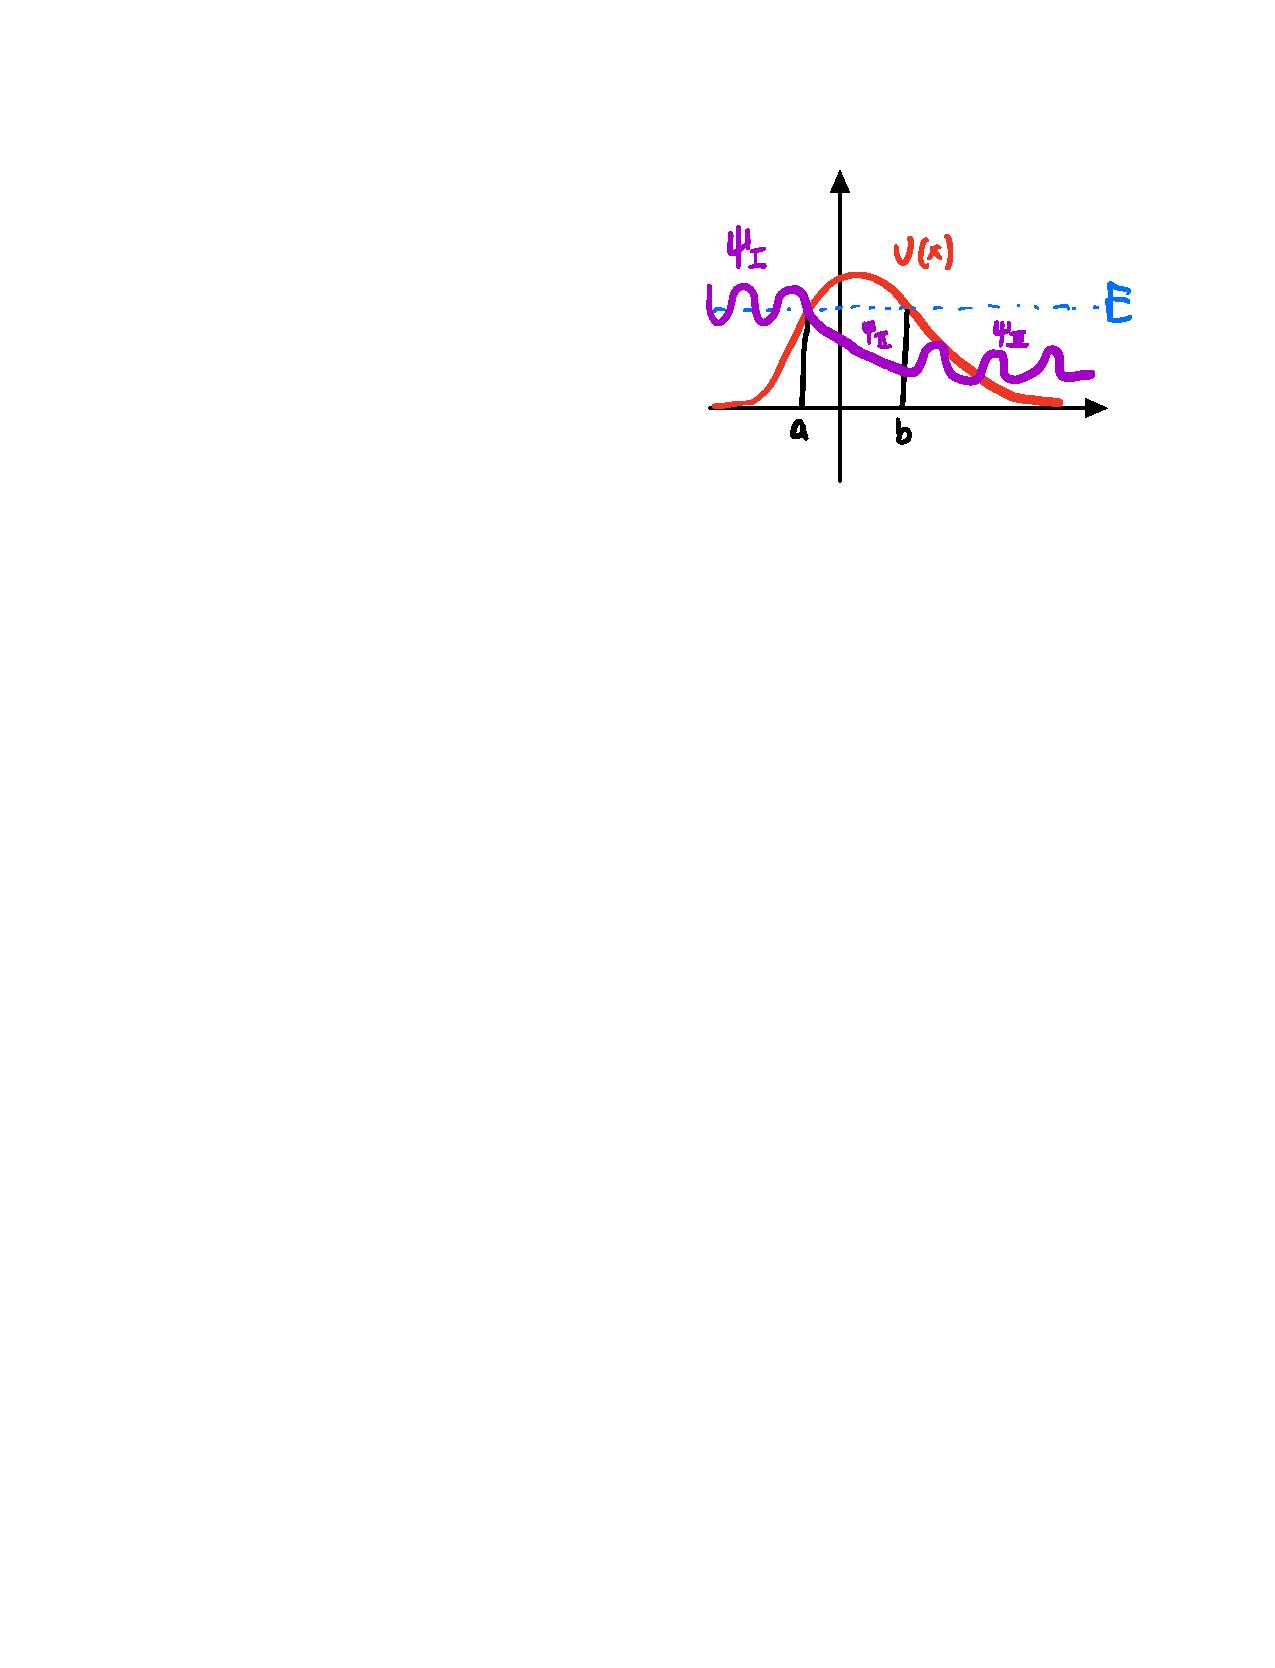
\includegraphics[]{Images/fig-WKBtunnelling.pdf}
    
    \caption{Using WKB to study quantum mechanical tunnelling. We have a particle incoming from the left in a classically allowed region, where the wavefunction is sinusoidal ($\psi_{I}$). In the classically forbidden region, the amplitude of the wavefunction exponentially decays ($\psi_{II}$). Finally, after the barrier, the wavefunction is again sinusoidal ($\psi_{III}$), but the amplitude is down exponentially from the wavefunction in the first region. We can use WKB and the connection formulas to obtain the approximate wavefunctions in each region, and find the transmission coefficient.}
    \label{fig-WKBtunnelling}
\end{figure}

Previously, we discussed getting the energy for an arbitrary potential:

\begin{figure}[htbp]
    \centering
    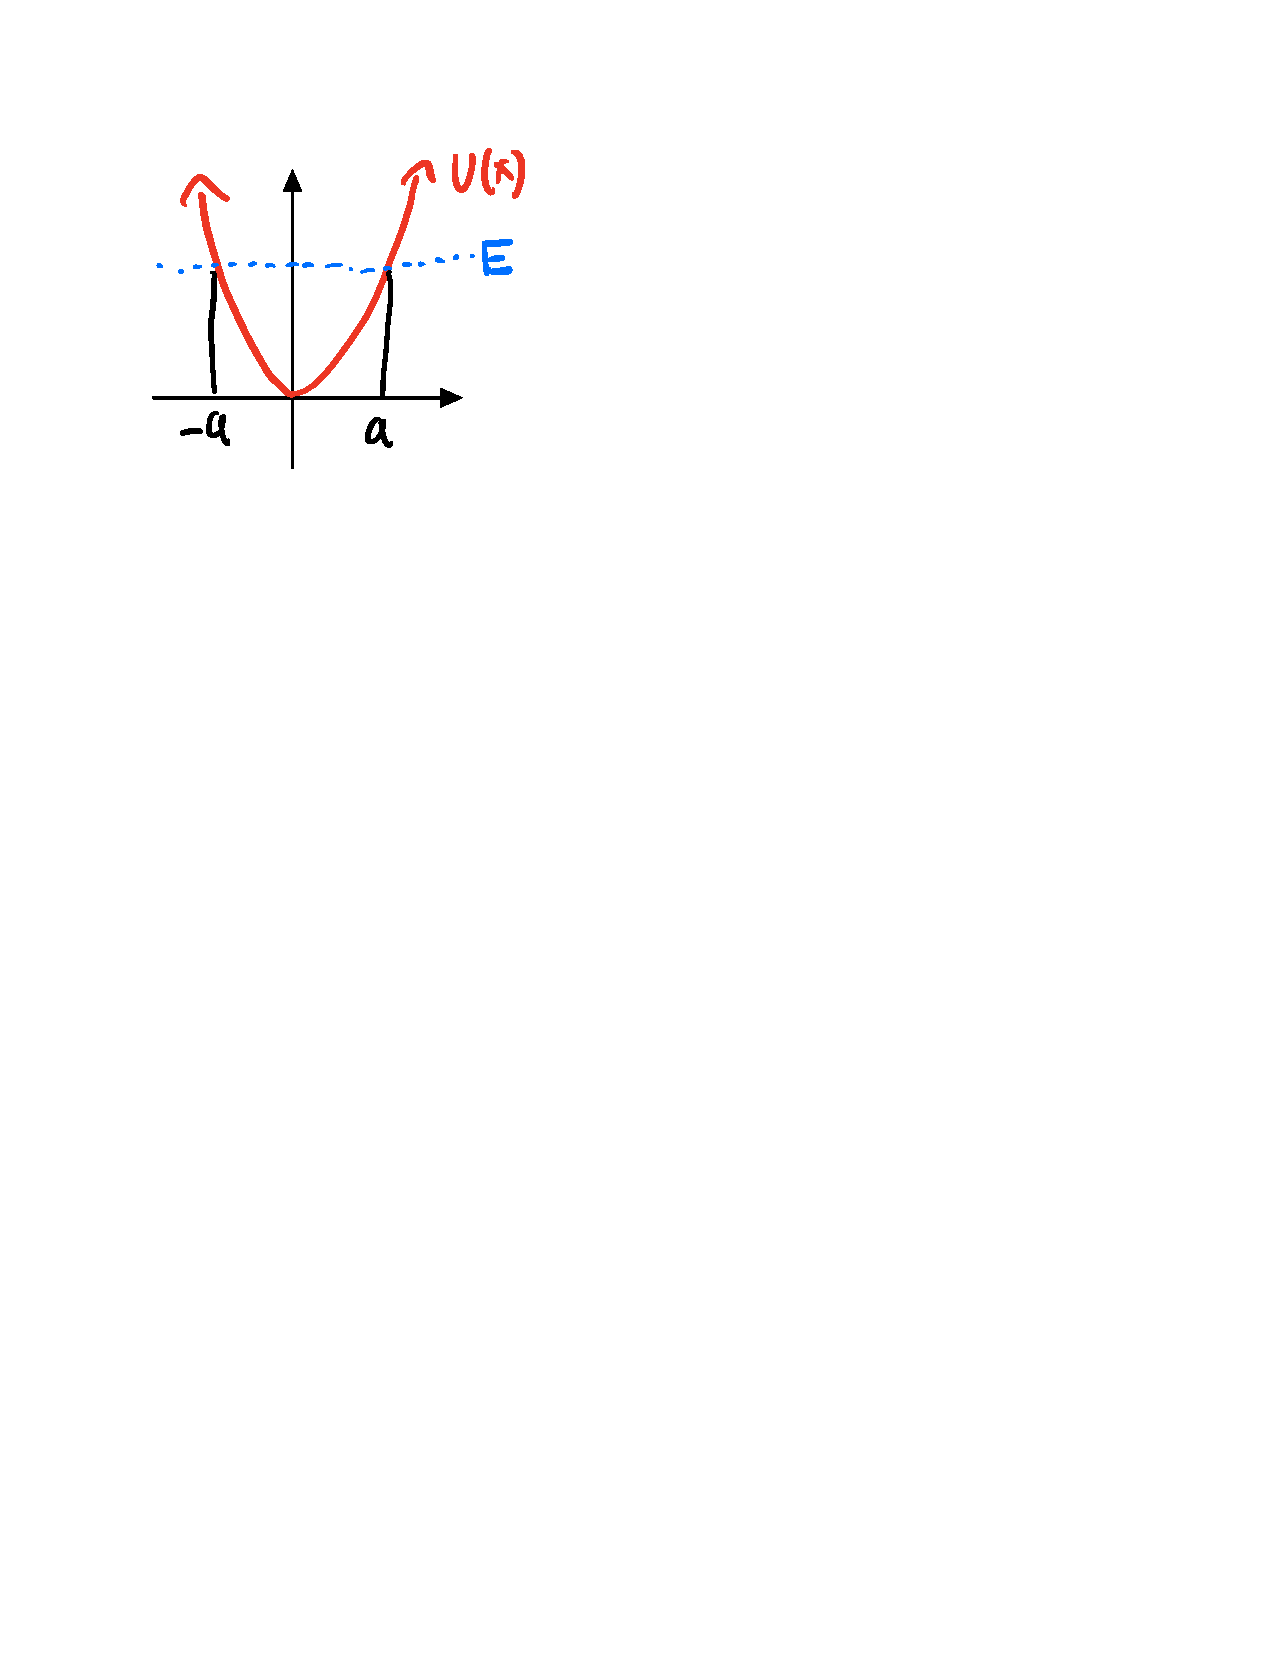
\includegraphics[scale=0.8]{Images/fig-WKBenergies.pdf}
    
    \caption{Last time, we found the energies of the Harmonic oscillator (quadratic potential) using the WKB approximation.}
    \label{fig-energyWKB}
\end{figure}


We considered carrying out the integral (classically):
\begin{equation}
    \int_{-a}^a \frac{pdx}{\hbar} = \pi(n + \frac{1}{2})
\end{equation}
Where $p^2/2m = E - U(x)$.

If we compare Fig. \ref{fig-tunnelling} and Fig. \ref{fig-energyWKB}, we can see in a hand-wavey way that we ``flip'' the potential between the two cases.

\subsection{Tunneling Derivation}
Using the WKB approximation, we can write the wavefunction in the three regions of Fig. \ref{fig-tunnelling} as:
\begin{equation}
    \psi_{III} = \frac{C}{\sqrt{p}} e^{i\int_b^x \frac{p(x')dx'}{\hbar} + \frac{i\pi}{4}}
\end{equation}
\begin{equation}
    \psi_{II} = \frac{C}{\sqrt{p}}e^{+\int_x^{b}\frac{pdx'}{\hbar}} + \frac{C}{\sqrt{p}}e^{-\int_x^b \frac{p(x')dx'}{\hbar}} = \frac{C}{\sqrt{p}}e^{\frac{p dx'}{\hbar}}
\end{equation}
We discard the second term in the above $\psi_{II}$ which is exponentially small, as the WKB approximation cannot recover exponentially small pieces. We are using the connection formula we derived previously to conclude that the $C$s are the same in the two formulas. We then write:
\begin{equation}
    \psi_{II} = \frac{C}{\sqrt{p}}e^{+\int_a^b\frac{pdx'}{\hbar}}e^{-\int_a^x \frac{pdx'}{\hbar}} = Ce^{\int_a^b \frac{pdx'}{\hbar}}\frac{1}{\sqrt{p}}e^{-\int_a^x \frac{pdx'}{\hbar}}
\end{equation}
The minus sign in the exponential means that the incoming particle from the right exponentially decays in the $II$ region. In $I, III$ the wavefunctions will be oscillatory. The question then becomes how much does the amplitude decrease between the two regions. Writing down the wavefunction in region $I$:
\begin{equation}
    \psi_I = \frac{D}{\sqrt{p}}\left[e^{+i\int_a^x \frac{p(x')dx'}{\hbar} + \frac{i\pi}{4}} + e^{-i\int_a^x \frac{p(x')dx'}{\hbar} - \frac{i\pi}{4}}\right]
\end{equation}
The transmission coefficient is:
\begin{equation}
    T = \frac{\abs{C}^2}{\abs{D}^2} = e^{-2\int_a^b \frac{p(x')dx'}{\hbar}}
\end{equation}
The reflection coefficient cannot actually be restored/computed using the WKB calculation, because we have discarded the exponentially supressed part in $\psi_{II}$. However, we can in general say $R = 1 - T$. 

When is the above formula is justified? When we have a highly excited state. Mathematically, this is when:
\begin{equation}
    \int_a^b \frac{pdx'}{\hbar} \gg 1.
\end{equation}
or when:
\begin{equation}
    T \ll 1.
\end{equation}
I.e. the transmission is very small. The WKB approximation fails when $E \approx U$, i.e. when the energy of the incoming particle is close to the height of the potential well. In this case there would not be a significant decay of the wavefunction inside of the well.

We will explore this on Q3 of the HW3.

\subsection{Motivating Time-Dependent Perturbation Theory}
Up until this point, we had a time-independent Hamiltonian $H$, and we could express the time evolution of an arbitrary state $\psi(x, t)$ as:
\begin{equation}
    \psi(x, t) = \sum_n c_n \psi_n e^{-i\frac{E_n t}{\hbar}}
\end{equation}
and if we had an eigenstate, there would be no time-evolution whatsoever. Of course this is not what happens in real life; a highly excited hydrogen atom state does not stay in this same state forever. We require the study of time-dependent perturbations for this, so let us begin.

\subsection{Developing Time-Dependent Perturbation Theory}
We consider a two-level system with Hamiltonian $H^{(0)}$ with eigenstates $\ket{\psi_a}, \ket{\psi_b}$ such that:
\begin{equation}
    H^{(0)}\ket{\psi_a} = E_a\ket{\psi_a}, \quad H^{(0)}\ket{\psi_b} = E_b\ket{\psi_b}
\end{equation}
\begin{equation}
    \bra{\psi_a}{\psi_b} = \delta_{ab}
\end{equation}
and the evolution of a general state was given by:
\begin{equation}\label{eq-psit}
    \ket{\psi(t)} = c_a\ket{\psi_a}e^{-i\frac{E_a t}{\hbar}}  + c_b\ket{\psi_b}e^{-i\frac{E_b t}{\hbar}}.
\end{equation}
Now we consider some time-dependent perturbation $H'(t)$, and we ask what the transition probability is. Let us try to figure it out. The total Hamiltonian is:
\begin{equation}
    H = H^{(0)} + H'(t)
\end{equation}
so we can write down the Schrodinger equation:
\begin{equation}
    i\hbar \dpd{\ket{\psi}}{t} = H\ket{\psi}
\end{equation}
Therefore evaluating the LHS for $\ket{\psi(t)}$ as in Eq. \eqref{eq-psit} we have:
\begin{equation}
    \begin{split}
        &i\hbar \dpd{\ket{\psi(t)}}{t}
        \\ &= i\hbar\dot{c}_a\ket{\psi_a}e^{-i\frac{E_at}{\hbar}} + i\hbar c_a\left(-i\frac{E_a}{\hbar}\right)\ket{\psi_a}e^{-i\frac{E_a t}{\hbar}}
        \\ &+ i\hbar\dot{c}_b\ket{\psi_b}e^{-i\frac{E_bt}{\hbar}} + i\hbar c_b\left(-i\frac{E_b}{\hbar}\right)\ket{\psi_b}e^{-i\frac{E_b t}{\hbar}}
    \end{split}
\end{equation}
Evaluating the RHS we then have:
\begin{equation}
    \begin{split}
        &H\ket{\psi(t)} 
        \\ &= c_aE_a\ket{\psi_a}e^{-i\frac{E_at}{\hbar}} + c_bE_b\ket{\psi_b}e^{-i\frac{E_b t}{\hbar}}
        \\ &+ H'c_a\ket{\psi_a}e^{-i\frac{E_a t}{\hbar}} + H'c_b\ket{\psi_b}e^{-i\frac{E_b t}{\hbar}}
    \end{split}
\end{equation}
We can cancel out the terms of the above that come from the SE with the time-independent Hamiltonian $H$ (i.e. the second column of terms on the LHS and the first row of terms on the RHS). Now, multiplying both sides on the right with $\bra{\psi_a}$ and using orthogonality, we find:
\begin{equation}
    i\hbar \dot{c}_a = c_a\bra{\psi_a}H'(t)\ket{\psi_a} + \bra{\psi_a}H'(t)\ket{\psi_b}c_b e^{-i\frac{E_b - E_a}{\hbar}t}
\end{equation}
and analogously for $\bra{\psi_b}$:
\begin{equation}
    i\hbar \dot{c}_b = c_b\bra{\psi_b}H'(t)\ket{\psi_b} + \bra{\psi_b}H'(t)\ket{\psi_a}c_a e^{-i\frac{E_a - E_b}{\hbar}t}
\end{equation}
So far we have not done anything approximate; everything has been analytic. We now make our first simplification; we consider:
\begin{equation}
    \bra{\psi_a}H'(t)\ket{\psi_a} = \bra{\psi_b}H'(t)\ket{\psi_b} = 0.
\end{equation}
as we are only interested in the transitions between the states (but it is trivial to generalize this to the case where the above are nonzero). With this our formulas simplify:
\begin{equation}
    \begin{split}
        \dot{c}_a &= \frac{-i}{\hbar}c_b \bra{\psi_a}H'(t)\ket{\psi_b}e^{-i\omega t}
        \\  \dot{c}_b &= \frac{-i}{\hbar}c_a\bra{\psi_b}H'(t)\ket{\psi_a}e^{i\omega t}
    \end{split}
\end{equation}
where $\omega = \frac{E_b - E_a}{\hbar}$. But note we have not made any assumptions about the weakness of our potentials, or anything like that. Note that solving the above formula is in general quite difficult to solve; so we will develop PT techniques for it.
\newpage
\section{Time-Dependent Perturbation Theory}
Let us review what we did last class (and not just the formula, but when the formula applies!) We had the Hamiltonian:
\begin{equation}
    H = H^0 + H'(t).
\end{equation}
In QM up until this point, the eigenstates $H^0$ were totally stable/stationary in time. But of course in nature this is not what happens; we have transitions of states. This is why we start to think about time-dependent Hamiltonians. We derived:
\begin{equation}
    \begin{split}
        \dot{c}_a &= -\frac{i}{\hbar}c_b \bra{\psi_a}H'\ket{\psi_b}e^{-i\omega t}
        \\ \dot{c}_b &= -\frac{i}{\hbar}c_a \bra{\psi_b}H'\ket{\psi_a}e^{i\omega t}
    \end{split}
\end{equation}
with:
\begin{equation}
    \omega = \frac{E_b - E_a}{\hbar}.
\end{equation}
The only simplification that went into this was $\bra{\psi_a}H'\ket{\psi_b} = 0$ (but this is harmless and we could do without it). Up until this point, we have made no assumptions. But let us enforce some now.

\subsection{First-Order Time-Dependent Perturbation Theory}
Let us assume $c_a(t = 0) = 1$ and $c_b(t = 0) = 0$ (though we can make an arbitrary choice of initial conditions). Now, we make an assumption that $c_b = 0$ and $c_a = 1$ in the above formula (i.e. in the above formulas we assume that the $c_b/c_a$ on the RHS are \emph{not} time dependent). We can then proceed to discuss corrections to this formula, but this involves higher orders of perturbation theory. The only differential equation we need to solve under this approximation is:
\begin{equation}
    \dot{c}_b = -\frac{i}{\hbar}\bra{\psi_b}H'(t)\ket{\psi_a}e^{i\omega t}
\end{equation}
Which has solution:
\begin{equation}
    c_b(t) = -\frac{i}{\hbar}\int_0^t dt' e^{i\omega t'}\bra{\psi_b}H'(t')\ket{\psi_a}
\end{equation}
The probability to find the state in the $b$ state is then nothing but:
\begin{equation}
    P_b(t) = \frac{1}{\hbar^2}\left|\int_0^t dt' e^{i\omega t'}\bra{\psi_b}H'(t')\ket{\psi_a}\right|^2
\end{equation}

\subsection{Second-Order Time-Dependent Perturbation Theory}
To second order, we consider plugging our first-order solution for $c_b(t)$ back into the $c_a(t)$ equation, so:
\begin{equation}
    \dod{c_a}{t} = -\frac{i}{\hbar}\bra{\psi_a}H'(t)\ket{\psi_b}e^{-i\omega t}\left(-\frac{i}{\hbar}\right)\int_0^t dt' e^{i\omega t'}\bra{\psi_b}H'(t')\ket{\psi_a}
\end{equation}
and so:
\begin{equation}
    c_a(t) = -\frac{1}{\hbar^2}\int_0^t dt' e^{-i\omega t'}\bra{\psi_a}H'(t')\ket{\psi_b}\int_0^{t'}dt'' e^{i\omega t''}\bra{\psi_b}H'(t'')\ket{\psi_a}
\end{equation}
The third order perturbation theory (and higher orders) follow by continuing to iterate as we have done above (solve for the coefficients at a lower order, then plug them back into the differential equation and solve). Formally, the full perturbative expansion can be written down as a Dyson series. But often the lower order terms are sufficient to probe interesting physical effects.

\subsection{Example: Exponentially Decaying Electric Field Pulse}
We consider a electric field with temporal profile:
\begin{equation}
    E(t) = E_0e^{-t^2/\tau^2}
\end{equation}
so our perturbing Hamiltonian is:
\begin{equation}
    H'(t) = -eE_0e^{-t^2/\tau^2}z
\end{equation}

\begin{figure}[htbp]
    \centering
    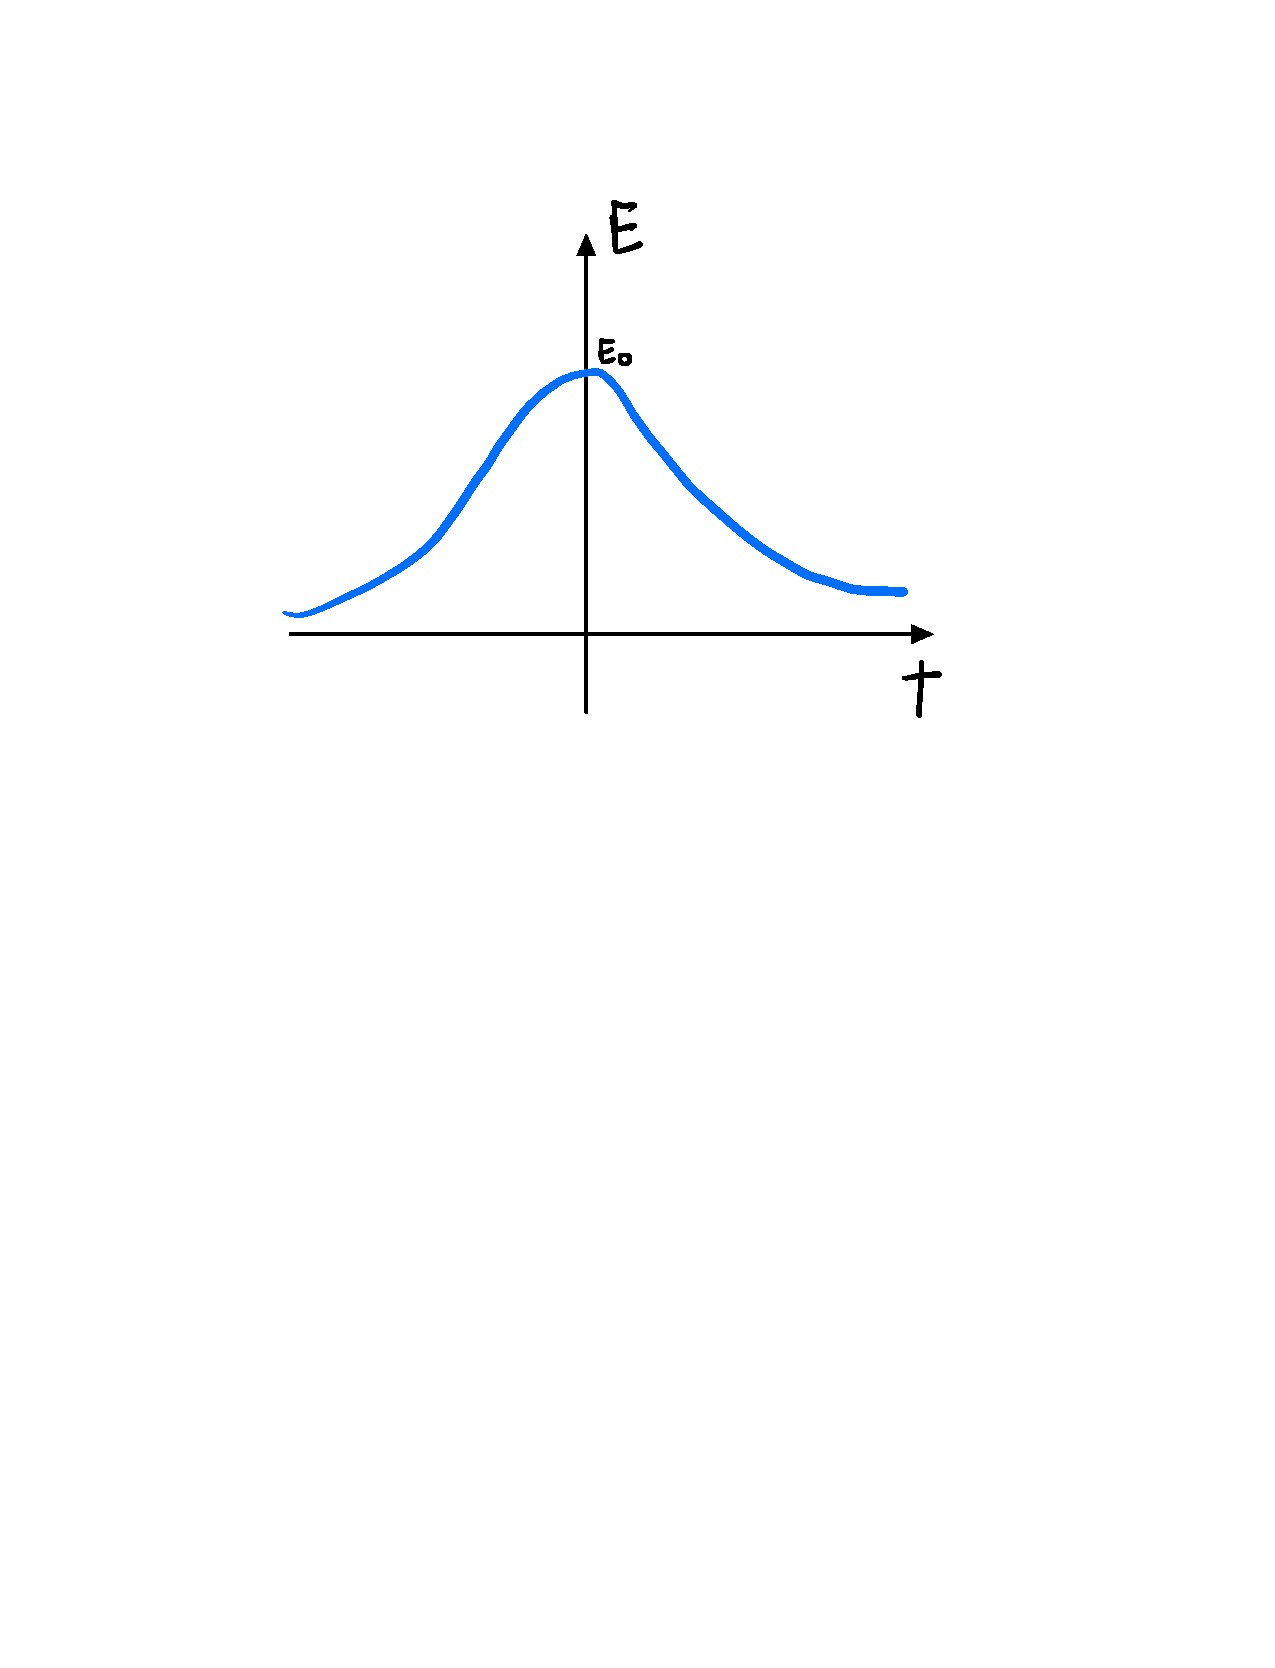
\includegraphics[scale=0.6]{Images/fig-gaussianpulse.pdf}
    \caption{Sketch of the gaussian pulse of the electric field.}
    \label{fig-gaussianpulse}
\end{figure}

We suppose that our state starts in the $\ket{100}$ state. We want to determine the transition probability to $\ket{n \neq 0, l = 1, m = 0}$ We recall from our selection rules that:
\begin{equation}
    \bra{nlm}z\ket{100} \neq 0
\end{equation}
in the case where $l = 1$ (different parity) and $m = 0$ (same magnetic quantum number). Using our first-order perturbation theory result. then find the transition coefficient of:
\begin{equation}
    c_b(t = \infty) = -\frac{i}{\hbar} \int_{-\infty}^\infty dt' e^{i\omega t'} e^{-t'^2/\tau^2}\left(-eE_0\avg{z}\right)
\end{equation}
Where $\avg{z} \sim a_B$. To compute the integral in the above, we complete the square:
\begin{equation}
    \int_{-\infty}^\infty dt' e^{i\omega t'} e^{-t'^2/\tau^2} = \int_{-\infty}^\infty dt' e^{\frac{1}{-\tau^2}\left(t' - \frac{i\tau^2\omega}{2}\right)^2}e^{\frac{1}{\tau^2}\left(\frac{i\tau^2\omega}{2}\right)^2} = \sqrt{\pi \tau^2}e^{-\frac{\tau^2\omega^2}{4}}
\end{equation}
where we have evaluated the integral by considering that it is nothing but the famous Gaussian. And so we find:
\begin{equation}
    \abs{c_b}^2 = \frac{\pi\tau^2}{\hbar^2}e^{-\frac{\tau^2\omega^2}{2}}\abs{\bra{nlm}z\ket{100}}^2
\end{equation}
The latter coefficient we can say is $a_B^2$ by dimensional consideration; we don't care that much about it:
\begin{equation}
    \abs{c_b}^2 = \frac{\pi\tau^2a_B^2}{\hbar^2}e^{-\frac{\tau^2\omega^2}{2}}
\end{equation}
Note that all of this was justified if:
\begin{equation}
    \abs{c_b}^2 \ll 1
\end{equation}
There are two cases of interest:
\begin{enumerate}
    \item $\omega \tau \gg 1$; i.e. the adiabatic approximation, where the external field changes very slowly. In this limit, this has no chance of actually causing a transition. We can see this from the formula but also physical intuition; the quickly changing degrees of freedom of the systems change must faster than the perturbation. As an example, atoms don't care about the (comparitively much slower) expansion of the universe! In this case, we have:
    \begin{equation}
        P_{a \to b}(t = \infty) \sim e^{-\tau^2\omega^2} \ll 1
    \end{equation}
    \item $\omega \tau \ll 1$; i.e. an instantaneous perturbation/a very short pulse. In this case, we have that the exponential term can be neglected (it is close to one) and so:
    \begin{equation}
        P_{a \to b} \sim \abs{\pi \tau^2 e^2 E_0^2 a^2}{\hbar^2} \ll 1
    \end{equation}
    And from the $\omega \tau \ll 1$ condition we can write:
    \begin{equation}
        P_{a \to b} \sim \abs{\pi \tau^2 e^2 E_0^2 a^2}{\hbar^2} \ll \frac{\pi e^2E_0^2 a^2}{\hbar^2\omega^2} = \frac{\pi e^2E_0^2 a^2}{(E_a - E_b)^2}
    \end{equation}
    where in the last equality we invoke the definition of $\omega$. Let's look at the physical meaning of this last expression:
    \begin{equation}
        \frac{\abs{eE_0a}}{E_a - E_b} \ll 1
    \end{equation}
    and so:
    \begin{equation}
        E_0 \ll \frac{10\si{eV}}{e 10^{-8}\si{cm}} = 10^9 \si{V.cm^{-1}}
    \end{equation}
    which is justified. We also note that the transition is most likely when the pulse timescale is on the same order as the frequency timescale (might have got this wrong - didn't quite follow).
\end{enumerate}

We will not discuss instantaneous perturbation theory much further. Usually, the way it is treated that you have one Hamiltonian and then at some time you turn on a new Hamiltonian suddenly. The system then does not have time to adjust to the new Hamiltonian, so you can expand the old state in terms of the new ones etc... There are many physical examples (e.g. $\beta$-decay). 

We will however explore the adiabatic approximation much further. There are many interesting implications here for condensed matter such as Berry phase, topological phases etc.

Next class, we discuss perturbation theory for the case when we have a periodic potential. After this, we discuss how to compute transitions.
\newpage
\section{Time-Dependent Perturbation Theory II}
We had eigenstates $\ket{\psi_a}, \ket{\psi_b}$ of a two-level system, with $c_a(t = 0) = 1, c_b(t = 0) = 0$. We then calculated (to first order in perturbation theory):
\begin{equation}
    c_b(t) = -\frac{i}{\hbar}\int_0^t dt' e^{i\omega_0 t'}\bra{\psi_b} H'\ket{\psi_a}
\end{equation}
where $\omega_0 = \frac{E_b - E_a}{\hbar}$. The transition probability was:
\begin{equation}
    P_b(t) = \abs{c_b(t)}^2
\end{equation}
and the perturbation theory was valid whenever $\abs{c_b(t)}^2 \ll 1$.

\subsection{Periodic Perturbation and Fermi's Golden Rule}
We consider a periodic perturbation of the form:
\begin{equation}
    H' = V(r)2\cos(\omega t)  = V(r)\left[e^{i\omega t} + e^{-i\omega t}\right]
\end{equation}
this is an absolutely crucial kind of perturbation; there are many periodic phenomena in physics, and even when not periodic, we can always Fourier transform and look at individual frequencies. A notational point that $\omega_0$ is the energy splitting of the two level system, and $\omega$ is an external parameter. We can immediately substitute this into the formula and find:
\begin{equation}
    c_b(t) = V_{ba}\left(-\frac{i}{\hbar}\right)\left[\int_0^t dt' e^{-i\omega t'}e^{i\omega_0 t} + e^{i\omega t'}e^{i\omega_0 t}\right]
\end{equation}
where $V_{ba} = \bra{\psi_b}V(r)\ket{\psi_a}$. The computation is simple:
\begin{equation}
    c_b(t) = -\frac{V_{ba}}{\hbar}\left[\frac{e^{i\omega_0 + \omega}t}{\omega_0 + \omega} + \frac{e^{i(\omega_0 - \omega)t}}{\omega_i - \omega}\right]
\end{equation}
The first term corresponds to spontaneous absorption and the second spontaneous emission. Let us assume that $\abs{\omega_0 - \omega} \ll \omega_0$ so we only consider the second term. We then find:
\begin{equation}
    c_b(t) = \frac{V_{ba}}{\hbar}\frac{e^{i\frac{\omega_0 - \omega}{2}}t}{\omega_0 - \omega}\left[2i\sin(\frac{\omega_0 - \omega}{2}t)\right]
\end{equation}
where we have used the identity $e^{i\alpha} - 1 = e^{i\frac{\alpha}{2}}\left(e^{i\frac{\alpha}{2}} - e^{-i\frac{\alpha}{2}}\right) = e^{i\frac{\alpha}{2}}2i\sin(\frac{\alpha}{2}) = -2e^{i\frac{\alpha}{2}}\sin(\frac{\alpha}{2})$. The probability is then:
\begin{equation}
    \abs{c_b(t)}^2 = \frac{4\abs{V_{ba}}^2}{\hbar^2(\omega_0 - \omega)^2}\sin^2\left(\frac{\omega_0 - \omega}{2}t\right)
\end{equation}
so the probability is seen to oscillate in time. We now make a mathematical claim:

\begin{equation}
    \lim_{t \to \infty}\frac{\sin^2(\alpha t)}{\pi t \alpha^2} = \delta(\alpha)
\end{equation}
with $\alpha = \frac{\omega_0 - \omega}{2}$ in our case. This limit is of interest as generally the timescale of experiments is much longer than the rapid fluctuations in the quantum systems. We now prove this. If $\alpha \neq 0$, then:
\begin{equation}
    \lim_{t \to \infty}\frac{\sin^2(\alpha t)}{\pi t \alpha^2} = 0
\end{equation}
as $\abs{\sin^2(\alpha t)} \leq 1$ and $\frac{1}{t} \to 0$. If $\alpha \to 0$, then:
\begin{equation}
    \lim_{t \to \infty} \lim_{\alpha \to 0}\frac{\sin^2(\alpha t)}{\pi t \alpha^2} = \lim_{t \to \infty} \lim_{\alpha \to 0}\frac{(\alpha t)^2}{\pi t \alpha^2} = \lim_{t \to \infty} \lim_{\alpha \to 0} \frac{t}{\pi} = \lim_{t \to \infty} \frac{t}{\pi} = \infty.
\end{equation}
We now consider:
\begin{equation}
    \int_{-\infty}^\infty \frac{\sin^2(\alpha t)}{\pi t^2\alpha^2} d(\alpha t) = \int_{-\infty}^\infty \frac{\sin^2 \eta}{\pi \eta^2}d\eta = \frac{1}{\pi} \cdot \pi = 1.
\end{equation}
so our function is indeed the delta function $\delta(\alpha)$.

So:
\begin{equation}
    P_b(t) = \frac{\abs{V_{ba}}^2}{\hbar^2}\left(\frac{\sin^2\alpha t}{\pi t \alpha^2} \right) \pi t \stackrel{t\to\infty}{\longrightarrow} \frac{\abs{V_{ba}}^2}{\hbar^2}\pi t \delta(\frac{\omega_0 - \omega}{2})
\end{equation}
now using the identity $\delta(\alpha x) = \frac{\delta(x)}{\abs{a}}$ we have:
\begin{equation}
    P_b(t) = \frac{\abs{V_{ba}}^2}{\hbar}2\pi t\delta(E_b - E_a - \hbar \omega)
\end{equation}
The probability per unit time is:
\begin{equation}
    \dod{W}{t} = \frac{2\pi}{\hbar}\abs{V_{ba}}^2\delta(E_b - E_a - \hbar\omega)
\end{equation}
which is \emph{Fermi's golden rule}.

The missing part is degeneracy. The rate of events is:
\begin{equation}
    R = \int \dod{W}{t}\frac{d^3pd^3x}{(2\pi\hbar)^3} = \int \frac{2\pi}{\hbar}\abs{V_{ba}}^2\delta(E_f - E_i + \hbar\omega) \cdot \frac{d^3pd^3x}{(2\pi\hbar)^3}
\end{equation}
(using that $\delta(-x) = \delta(x)$). We have a number of states term on the right, which we derived from WKB.

$\int d^3x$ can be taken to be the volume $V$, and $d^3p$ can taken to be:
\begin{equation}
    d^3p = \hbar^3 d^3k = \hbar^3 k^2 dk d\Omega = \frac{\hbar^3 \omega^2d\omega}{c^3} d\Omega = \frac{\hbar^3\omega^3d(\omega h)}{c^3\hbar}d\Omega
\end{equation}

We now substitute this in, integrating out the delta function:
\begin{equation}
    \begin{split}
        dR &= \frac{2\pi}{\hbar}\abs{V_{ab}}^2 \frac{V\hbar^2\omega^2}{(2\pi\hbar)^3c^3}d\Omega 
        \\ &= \frac{\omega^2}{(2\pi)^2}\frac{d\Omega}{\hbar c^3}\abs{V_{ba}}^2 V
    \end{split}
\end{equation}
where the above is the rate per unit angle. But often the $d$ is dropped and this is just written as $R$.

We have yet to compute $\abs{V_{ab}}^2$, which is the most difficult part. Writing down the Hamiltonian:
\begin{equation}
    \hat{H} = \frac{\left(\hat{p} + \frac{e}{c}\hat{A}\right)^2}{2m}
\end{equation}
where we have set the charge $q = -e$. Next class we discuss the interactions between $\hat{A}$ and $\hat{p} = -i\hbar \nabla$, and derive different transitions. Interestingly, we will reproduce the dipole transitions we have seen in classical physics. 
\newpage
\section{Spontaneous Emission I}
The most important formula we derived last class is Fermi's golden rule, which reads:
\begin{equation}
    \dod{W}{t} = \frac{2\pi}{\hbar}\abs{V_{ba}}^2\delta(E_f - E_i)\frac{d^3pd^3x}{(2\pi\hbar)^3}
\end{equation}
We consider $\frac{d^3pd^3x}{(2\pi\hbar)^3} = \dod{N}{E}dE$ and then we integrate with respect to energy to remove the delta function.

\subsection{Deriving Transitions}
Now, we want to discuss the difficult matrix element part. We have the coupling Hamiltonian:
\begin{equation}
    H = \frac{\left(\v{p} + \frac{e}{c}\v{A}\right)^2}{2m} = \frac{\v{p}^2}{2m} + \frac{e}{2mc}\left(\v{A}\cdot \v{p} + \v{p} \cdot \v{A}\right) + \mathcal{O}(\v{A}^2)
\end{equation}
We use the Coloumb gauge $\nabla \cdot \v{A} = 0$. Note this is a different gauge from what you may see in quantum field theory, where we choose Lorentz invariant Gauges. This choice of Gauge allows us to simplify:
\begin{equation}
    H = \frac{\v{p}^2}{2m} + \frac{e}{2mc}\left(2\v{p}\cdot\v{a}\right)
\end{equation}
The potential is then:
\begin{equation}
    V(\v{r}) = \frac{e}{mc}\v{p} \cdot \v{A}
\end{equation}
We have the vector potential:
\begin{equation}
    \v{A} = \v{A}_0(r)e^{-i\omega t} + \text{h.c.}
\end{equation}
where h.c. denotes the Hermitian conjugate of the first term. We consider:
\begin{equation}
    \v{A}_0 = A_0\gv{\e}e^{i\v{k} \cdot \v{r}}
\end{equation}
where $\gv{\e}$ is the polarization. We have split the plane wave into a spatial ($e^{i\v{k} \cdot \v{r}}$) and time ($e^{-i\omega t}$) piece. 

Now we will cheat\footnote{``I am an honest man, but now I am cheating'' - Ariel 2022}. In quantum mechanics, we never ever discuss the creation or annhilation of states. The number of states is fixed. Technically we need quantum field theory to discuss such transitions; but we take the semi-classical approach followed in Goswami.

We also consider the EM Hamiltonian:
\begin{equation}
    H_{EM} = \frac{1}{8\pi}\left(\v{E}^2 + \v{B}^2\right)
\end{equation}
where we have written the above in Gaussian units (in SI, the terms would be $\frac{\e_0}{2}\v{E}^2 + \frac{1}{2\mu_0}\v{B}^2$). This has the benefit of placing the electric and magnetic fields on equal footing (same energy). We therefore compute the electric and magnetic fields in our Gauge:
\begin{equation}
    \v{E} = -\frac{1}{c}\dpd{\v{A}}{t} = \frac{i\omega}{c}A_0\gv{\e}e^{-i(\omega t - \v{k} \cdot \v{r})} + \text{h.c.}
\end{equation}
\begin{equation}
    \v{B} = \nabla \times \v{A} = i(\v{k} \times \gv{\e})A_0e^{-i(\omega t - \v{k} \cdot \v{r})} + \text{h.c.}
\end{equation}

Now the cheating enters. We say that:
\begin{equation}
    \int H_{EM}d^3x = \hbar \omega
\end{equation}
everything is classical on the LHS, but the RHS is quantum. Our normalization is that the plane wave in the entire volume is normalized to a single photon with frequency $\omega$. The proper way to do it (in quantum field theory) is to quantize the electric field, but we shortcut. Computing the integral:
\begin{equation}
    \int H_{EM}d^3x = \frac{2}{8\pi}\left(\frac{\omega^2}{c^2}\abs{A_0}^2 + \left(\v{k} \times \gv{\e}_0\right)^* \cdot \left(\v{k} \times \gv{\e}_0\right)\abs{A_0}^2\right) d^3x
\end{equation}
We compute the dot product as:
\begin{equation}
    \left(\v{k} \times \gv{\e}_0\right)^* \cdot \left(\v{k} \times \gv{\e}_0\right) = \v{k}^2\abs{\gv{\e}}^2 - (\v{k} \cdot \gv{\e})(\text{h.c.})^*
\end{equation}
Now note that $\v{k} \cdot \gv{\e} = 0$ as $\v{k} \cdot \v{A} \sim \nabla \cdot \v{A} = 0$. And so:
\begin{equation}
    \left(\v{k} \times \gv{\e}_0\right)^* \cdot \left(\v{k} \times \gv{\e}_0\right) = \left(\frac{\omega}{c}\right)^2
\end{equation} 
so the integral becomes:
\begin{equation}
    \int H_{EM}d^3x = \frac{2}{8\pi}B\abs{A_0}^2\left(\frac{\omega^2}{c^2}\right)2 = \frac{V\abs{A_0}^2}{2\pi c^2}\omega^2 = \hbar\omega
\end{equation}
We therefore conclude:
\begin{equation}
    \boxed{\abs{A_0}^2 = \frac{2\pi c^2 \hbar}{\omega V}}
\end{equation}
Now let's look at the coupling part of the problem:
\begin{equation}
    V(r) = \frac{e}{mc}\v{p} \cdot \v{A} = \frac{e}{mc}\sqrt{\frac{2\pi c^2\hbar}{\omega V}}\gv{\e}e^{-i\v{k \cdot \v{r}}} \cdot \v{p}
\end{equation}
We now compute the matrix elements:
\begin{equation}
    \bra{\psi_a}\gv{\e} \cdot \v{p}e^{-i\v{k}\cdot \v{r}}\ket{\psi_b}\left(\frac{e}{mc}\right)\sqrt{\frac{2\pi\hbar c^2}{\omega V}}
\end{equation}
We then consider that:
\begin{equation}
    \abs{V_{ab}}^2\frac{d^3p d^3x}{(2\pi\hbar)^3} \to \dod{N}{E}dE \abs{V_{ab}}^2 \sim \frac{V}{V}
\end{equation}
so we see that the volume drops out! After this we can just ignore the volume entirely, now we have seen how it precisely drops out.

We already discussed how $\gv{\e} \cdot \v{k} = 0$. Suppose $\v{k} = \frac{\omega}{c}(0, 0, \zhat)$. We have multiple options for polarizations. We have $\gv{\e}^x = (1, 0, 0), \gv{\e}^y = (0, 1, 0)$, and we can also take linear combinations, e.g. the circular polarizations $\gv{\e}^+ = \frac{1}{\sqrt{2}}(1, i, 0)$, $\gv{\e}^- = \frac{1}{\sqrt{2}}(1, -i, 0)$. We call $\gv{\e}^+$ right handed and $\gv{\e}^-$ left handed. In particle physics/condensed matter, we say that it is right or left handed from the perspective of the detector. To see this:
\begin{equation}
    \v{E} = (\xhat + i\yhat)e^{-i(\omega t + ikz)} + \text{h.c.} \sim \xhat\cos(\omega t - kz) + \yhat\sin(\omega t - kz)
\end{equation}
and one can see that the wave rotates to the right, following the peak.

\begin{figure}[htbp]
    \centering
    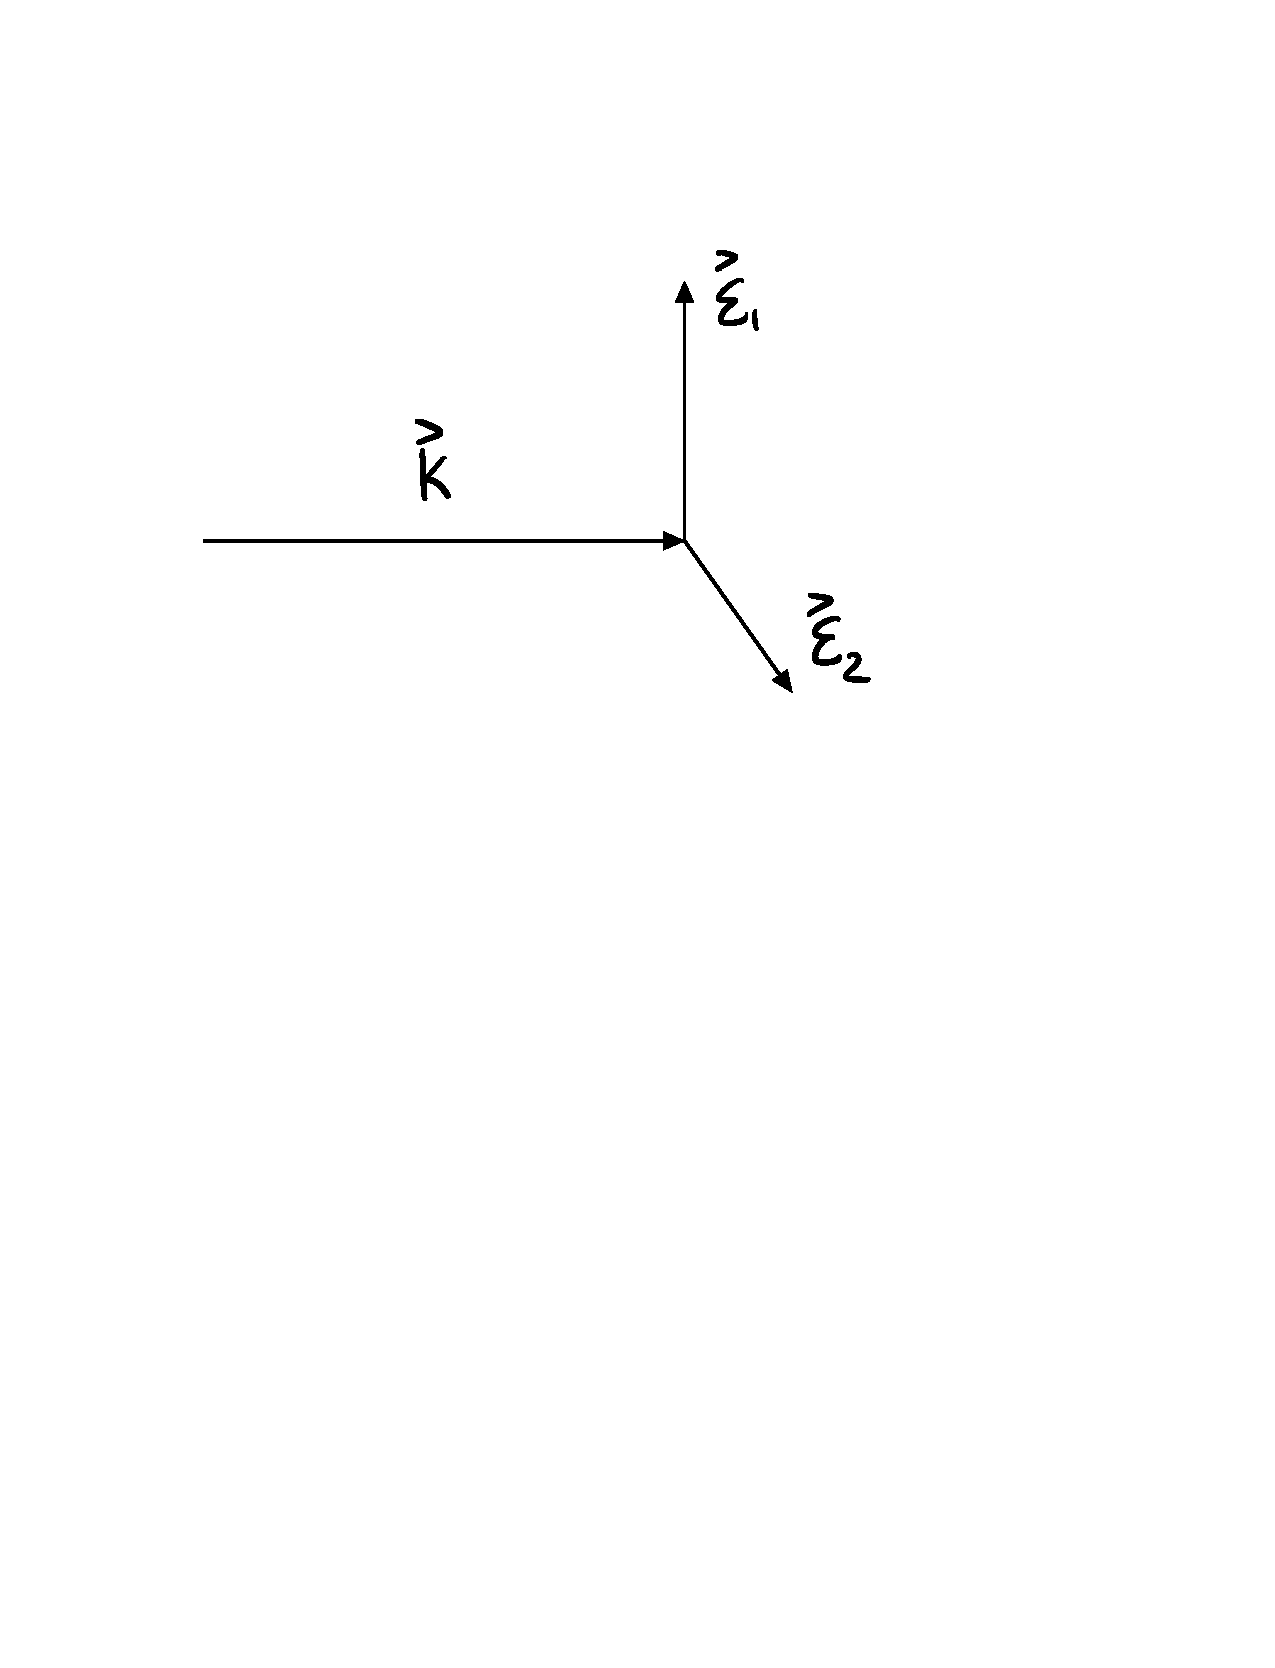
\includegraphics[scale=0.6]{Images/fig-photonpolarizations.pdf}
    \caption{We have two polarization vectors $\gv{\e}_1, \gv{\e}_2$ that are perpendicular to the direction of propogation $\v{k}$. We may take superpositions of these to construct (e.g.) circular polarized light.}
    \label{fig-photonpolarizations}
\end{figure}

Let us write down the formula with everything discussed:
\begin{equation}
    \dod{W}{t} = \int \sum_\lambda \left(\frac{2\pi}{\hbar}\right)\left(\frac{e}{mc}\right)\left(\sqrt{\frac{2\pi\hbar c^2}{\omega V}}\right)^2 \left|\bra{f}e^{-i\v{k} \cdot \v{r}}\gv{\e} \cdot \v{p}\ket{i}\right|^2\delta(E_+ - E_-)\frac{d^3pV}{(2\pi\hbar)^3}
\end{equation}
where $\sum_\lambda$ is the sum over polarizations. We will cheat one more time and borrow something from QFT. We expand in a sum over modes:
\begin{equation}
    \v{A} = \sum_{\lambda, \v{k}}\sqrt{\frac{2\pi\hbar c^2}{\omega V}}\left[\gv{\e}_\v{k}^\lambda e^{-i(\omega t - \v{k} \cdot \v{r})}a_{\v{k}, \lambda} + \gv{\e}^{*\lambda}_\v{k}e^{i(\omega t - \v{k} \cdot \v{r})}a^\dag_{\v{k}, \lambda}\right]
\end{equation}
where we have replaced the coefficients (numbers) $a_\v{k, \lambda}/a^*_\v{k, \lambda}$ with operators $a_\v{k}/a^\dag_\v{k}$ which annihilate/create photons respectively. In the diagonal form we may write:
\begin{equation}
    H = \sum_{\v{k}}\hbar\omega \left(a^\dag_{\v{k}}a_\v{k} + \frac{1}{2}\right)
\end{equation}
(there are deep hidden things here... e.g. the above energy is infinite because of the $+\frac{1}{2}$ - this puzzled physicists indeed. Related to things like Caismir effect).

We therefore consider the creation of a single photon to consider $\bra{\gamma}a^\dag_{\v{k}, \lambda}\ket{0} = 1$. What remains is to evaluate $\left|\bra{f}e^{-i\v{k} \cdot \v{r}}\gv{\e} \cdot \v{p}\ket{i}\right|^2 = 1$. 

$ka_b \sim 10^{-3}$, then $ka_B \sim \frac{\hbar\omega}{me^2c} = \frac{e^2}{\hbar c} = \alpha$ where we take $\hbar\omega$ to be a Rydberg. Why we use perturbation theory in $\alpha$ is because it is small. We will do a multiple expansion in $\alpha$ to determine transitions. We will do this next way and formulate selection rules.
\newpage
\section{Spontaneous Emission II}
We derived the formula for the probablity per unit time:
\begin{equation}
    \dod{W}{t} = \sum_\lambda \frac{1}{2\pi\hbar c^3}\left(\frac{e}{m}\right)^2\omega\abs{\bra{f}\gv{\e}^\lambda \cdot \v{p}\ket{i}}^2d\Omega
\end{equation}

\subsection{Finishing the Rate Calculation}
We now do the computation of the matrix element. Note that the polarization does not influence the matrix element at all, so:
\begin{equation}
    \bra{f}\gv{\e}^\lambda \cdot \v{p}\ket{i} = \gv{\e}^\lambda \cdot \bra{f}\v{p}\ket{i}
\end{equation}
We consider the Hamiltonian:
\begin{equation}
    H^0 = \frac{\v{p}^2}{2m} - \frac{e^2}{r}
\end{equation}
Then the commutator of $H^0$ with position is:
\begin{equation}
    [H^0, x_j] = [\frac{p_ip_i}{2m}, x_j] = \frac{p_i}{2m}[p_i, x_j]2 = -\frac{2p_i}{2m}\left(-i\hbar\delta_{ij}\right) = \frac{i\hbar}{m}p_j
\end{equation}
Now let us represent:
\begin{equation}
    p_j = \frac{m}{\hbar i}[H^0, x_j]
\end{equation}
So substituting this into our rate:
\begin{equation}
    \dod{W}{t} = \sum_\lambda \frac{1}{2\pi\hbar c^3}\left(\frac{e}{m}\right)^2\omega\left(\frac{m}{\hbar}\right)^2\abs{\gv{\e}^\lambda \cdot \bra{f}[H^0, x_i]\ket{i}}^2d\Omega
\end{equation}
this commutator is very easy, as it just gives an energy difference:
\begin{equation}
    \begin{split}
        \dod{W}{t} &= \sum_\lambda \frac{1}{2\pi\hbar c^3}\left(\frac{e}{m}\right)^2\omega\left(\frac{m}{\hbar}\right)^2\abs{\gv{\e}^\lambda \cdot (E_f - E_i)\bra{f}\v{x}\ket{i}}^2d\Omega
        \\ &= \sum_\lambda \frac{1}{2\pi\hbar^2c^3}e^2\omega^3\abs{\gv{\e}^\lambda\cdot\bra{f}\v{x}\ket{i}}^2d\Omega
        \\ &= \sum_\lambda \frac{e^2\omega}{2\pi\hbar c}\abs{\gv{\e}^\lambda \bra{f}\v{x}\ket{i}k}^2
    \end{split}
\end{equation}
We estimate $kx \sim \frac{\omega}{c}a_B \sim \alpha \ll 1$. So:
\begin{equation}
    \begin{split}
        \dod{W}{t} = \sum_\lambda \frac{\alpha}{2\pi}\omega \abs{\gv{\e}^\lambda \cdot \abs{\v{k}}\bra{f}\v{x}\ket{i}}^2 = \sum_\lambda \frac{1}{2\pi}\frac{\omega}{\hbar c}\abs{\gv{\e}^\lambda \cdot \abs{\v{k}}\bra{f}\v{x}e\ket{i}}^2
    \end{split}
\end{equation}
Where $\v{x}e$ is the dipole moment operator - so these are electric dipole transitions!

\subsection{Estimating and Justifying Electric Dipole Transistions}
Since $ka_B \sim \frac{\omega}{c}a_B \sim \alpha$, then:
\begin{equation}
    \dod{W}{t} \sim \frac{\alpha}{2\pi}\omega \alpha^2 \sim \frac{\alpha^3}{2\pi}\omega
\end{equation}
Note that to check if the PT is justified, we check that our parameters are small when compared to the characteristic fluctuation time of the system:
\begin{equation}
    \dod{W}{t}\frac{1}{\omega} \sim \alpha^3 \ll 1
\end{equation}
this is indeed the case so it is justified. We are discussing UV light typically here, so a typical rate (with $\frac{\alpha^3}{2\pi} \sim 10^{-7}$, $\omega \sim \frac{10\si{eV}}{\hbar}$ with $\hbar = 6.6\times 10^{-16}\si{eVs}$:
\begin{equation}
    \dod{W}{t} \sim \frac{\alpha^3}{2\pi}\omega \sim 10^{-7}\frac{10\si{eV}}{ 6.6\times 10^{-16}\si{eVs}} \sim 10^9 \si{s^{-1}}.
\end{equation}
So, we have a billion transitions per second.

\subsection{Computing the Electric Dipole Transition}
We use some common tricks used by HEP folkks to carry out the formal calculation. The polarization is very irritating, as there are two polarizations per direction of propogation, and then we integrate over all angles... very messy. 
\begin{equation}
    \sum_\lambda \e_i^\lambda \e_j^\lambda(\v{n}) = A\delta_{ij} + Bn_in_j
\end{equation}
since we sum over polarizations, the information about it disappears. We only end up with a $\delta_{ij}$ and the product of photon momentum. There is nothing else in my life :(

Now we consider some conditions to evaluate what A, B are. Let us multiply both sides by $\delta_{ij}$. Since $\abs{\e}^2 = 1$ (as the polarizations are unit vectors) we end up with:
\begin{equation}
    2 = 3A + B
\end{equation}
If we multiply both sides by $n_in_j$, using that $\gv{\e} \cdot \v{k} = 0$, the LHS vanishes and so:
\begin{equation}
    0 = A + B
\end{equation}
Therefore:
\begin{equation}
    A = 1, B = -1
\end{equation}
and so:
\begin{equation}
    \sum_\lambda \e_i^\lambda \e_j^\lambda(\v{n}) = \delta_{ij} - n_in_j
\end{equation}
The probability per unit time after summing over all polarizations is then:
\begin{equation}
    \dod{W}{t} = \frac{\alpha}{2\pi}\omega\abs{\v{k}}^2\left[\bra{f}x_i\ket{i}\bra{i}x_j\ket{f}\right](\delta_{ij} - n_in_j)d\Omega
\end{equation}
This integral over all angles is something we have already done:
\begin{equation}
    \int(\delta_{ij} - n_in_j)d\Omega = \delta_{ij}4\pi - \frac{1}{3}\delta_{ij}4\pi = \delta_{ij}\left(4\pi - \frac{4\pi}{3}\right)
\end{equation}
Thus (after integrating):
\begin{equation}
    \dod{W}{t} = \frac{\alpha}{2\pi}\omega\abs{\v{k}}^2\left[\bra{f}x_j\ket{i}\bra{i}x_j\ket{f}\right]\frac{8\pi}{3}
\end{equation}
And just playing with the constants:
\begin{equation}
    \dod{W}{t} = \frac{4}{3}\frac{\omega}{\hbar c}\left(\frac{\omega}{c}\right)^2\abs{\bra{f}\v{d}\ket{i}}^2
\end{equation}
with $\v{d} = e\v{x}$ the dipole operator. Phrasing this in terms of intensity (from classical physics) we have:
\begin{equation}
    \dod{I}{t} = E\dod{W}{t} = \hbar\omega \dod{W}{t} = \frac{4}{3}\frac{\omega^4}{c^3}\abs{\bra{f}\v{d}\ket{i}}^2
\end{equation}
when we have a dipole oscillating as $\v{d} \sim e^{i\omega t}\v{d}_0$ (so $\ddot{\v{d}} = \omega^2\v{d}_0$), we can then represent:
\begin{equation}
    \dod{I}{t} = \frac{4}{3}\frac{1}{c^3}\abs{\bra{f}\ddot{\v{d}}\ket{i}}^2
\end{equation}
If we then identify $\bra{f}\v{d}\ket{i}$ as $\v{d}_{\emph{classical}}$ we see that we have the exact same formula as we would derive in classical physics (where we would integrate the poynting vector over a sphere).

\subsection{Selection Rules}
Previously when discussing the Stark effect we derived $\bra{f}z\ket{i}$. Noticing that $[L_z, z] = 0$, then:
\begin{equation}
    \bra{l', m'}L_zz - zL_z\ket{l, m} = 0
\end{equation}
so:
\begin{equation}
    (m'-m)\bra{l',m'}z\ket{l,m}.
\end{equation}
So the matrix element vanishes unless $m = m'$. Now we generalize this to $x \pm iy$. We have that $[L_z, x\pm iy] = \pm(x \pm iy)$. Going through the same steps:
\begin{equation}
    \bra{l',m'}L_z(x+iy) - (x+iy)L_z\ket{l, m} = \bra{l',m'}x+iy\ket{l,m}
\end{equation}
so:
\begin{equation}
    (m'-m-1)\bra{l',m'}x+iy\ket{l,m} = 0.
\end{equation}
So $m' = m + 1$. Of course the $l' = l \pm 1$ selection rule also holds.

\end{document}